\باب{لامتناہی تسلسل}
اس باب میں ہم ایک حیران کن کلیہ اخذ کرتے ہیں جس کی مدد سے بہت سارے تفاعل کو "لامتناہی کثیر رکنی" کی صورت میں لکھنا ممکن ہو گا اور ساتھ ہی کثیر رکنی کے  ارکان حذف  کر کے کثیر رکنی کو متناہی بنانے سے پیدا خلل بھی جان پائیں گے۔ ان تسلسل کو طاقتی تسلسل کہتے ہیں۔ قابل تفرق تفاعل کو تخمینی طور پر کثیر رکنی سے ظاہر کرنے میں مدد دینے کے علاوہ طاقتی تسلسل دیگر مواقع پر بھی کار آمد ثابت ہوتے ہیں۔ غیر بنیادی تکمل کی قیمت کے حصول کے علاوہ حراری توانائی کی منتقلی، ارتعاش، کیمیائی نفوذ اور ترسیل اشارات کے تفرقی مساوات  کے حل میں یہ موثر کردار ادا کرتے ہیں۔ آپ یہاں وہ ان تفاعل کے بارے میں سیکھ پائیں گے جو سائن اور انجینئری میں بہت زیادہ استعمال ہوتے ہیں۔

\حصہ{اعداد کی ترتیب کی حد}
غیر رسمی طور پر ترتیب سے مراد مرتب چیزوں کا سلسلہ ہے۔ اس باب میں ہمیں اعداد کی ترتیب سے غرض ہو گا۔ ترکیب نیوٹن سے حاصل اعداد کی ترتیب   \عددی{x_0,x_1,\cdots,x_n,\cdots} یا (ہلگے ون کوچ کے) برفانی روئی کے کثیر الاضلاع کی ترتیب \عددی{c_1,c_2,\cdots,c_n,\cdots} ہم دیکھ چکے ہیں۔ ان ترتیبوں کی حد پائی جاتی ہے، البتہ بہت سارے اہم ترتیبوں کے حد نہیں پائے جاتے ہیں۔

\جزوحصہء{تعریف اور علامتیت}
ہم \عددی{3} کے  ہر عدد صحیح مضرب کو ایک مقام مختص کر کے ایک فہرست بنا سکتے ہیں:
\begin{align*}
\begin{array}{rcccccc}
\text{\RL{دائرہ کار}} &1&2&3&\cdots&n&\cdots\\
\text{\RL{سعت}} &3&6&9&&3n&
\end{array}
\end{align*}
پہلا عدد \عددی{3}، دوسرا \عددی{6}، تیسرا \عددی{9}، وغیرہ، وغیرہ ہیں۔ مختص کرنے کا عمل ایک تفاعل ہے جو \عددی{n} ویں مقام کو \عددی{3n} مختص کرتا ہے۔ ترتیب کی بناوٹ کا بنیادی تصور یہی ہے۔ ایک تفاعل ہمیں بتاتا ہے کہ کس مقام پر کونسا عدد ہو گا۔

\ابتدا{تعریف}
ایک تفاعل جس کا دائرہ کار کسی عدد صحیح \عددی{n_0} کے برابر یا اس سے بڑے عدد صحیح پر مشتمل اعداد کا سلسلہ ہو \اصطلاح{لامتناہی ترتیب}\فرہنگ{ترتیب!لامتناہی}\حاشیہب{infinite sequence}\فرہنگ{sequence!infinite} (یا \اصطلاح{ترتیب}\فرہنگ{ترتیب}\حاشیہب{sequence}\فرہنگ{sequence})  کہلاتا ہے۔
\انتہا{تعریف}
%================

عموماً \عددی{n_0=1} ہوتا ہے اور ترتیب کا دائرہ کار مثبت اعداد صحیح پر مشتمل ہو گا۔ البتہ بعض اوقات ہم تسلسل کو کسی دوسرے عدد صحیح سے شروع کرنا چاہتے ہیں۔ ترکیب نیوٹن میں ہم \عددی{n_0=0} لیتے ہیں۔ اگر ہم \عددی{n} اضلاع پر مشتمل کثیر الاضلاع کی ترتیب کی بات کریں تب ہم \عددی{n_0=3} منتخب کرنا چاہیں گے۔

ترتیب کی تعریف کسی بھی تفاعل کی طرح کی جاتی ہے (مثال \حوالہ{مثال_تسلسل_متعدد_ترتیبات} اور شکل \حوالہ{شکل_تسلسل_مرتکز_منفرج_الف} تا شکل \حوالہ{شکل_تسلسل_مرتکز_منفرج_ث})، مثلاً:
\begin{align*}
a(n)=\sqrt{n},\quad a(n)=(-1)^{n+1}\frac{1}{n},\quad a(n)=\frac{n-1}{n}
\end{align*}

یہ ظاہر کرنے کی خاطر کہ دائرہ کار عدد صحیح ہے، ہم حرف \عددی{n} استعمال کرتے ہیں نا کہ دیگر غیر تابع متغیر کے لئے مستعمل حروف \عددی{x}، \عددی{y}، \عددی{z}، \عددی{t}، وغیرہ۔  مذکورہ بالا کی طرح تعریفی قاعدہ میں کلیات عموماً مثبت عدد صحیح سے زیادہ بڑے دائرہ کار کے لئے درست ہوتے ہیں۔ جیسا ہم دیکھیں گے یہ بعض اوقات سود مند ثابت ہوتا ہے۔ 

عدد \عددی{a(n)} ترتیب کا \اصطلاح{\عددی{n} واں جزو} یا اشاریہ \عددی{n} والا جزو ہو گا۔ اگر \عددی{a(n)=\tfrac{n-1}{n}} ہو تب درج ذیل ہو گا۔
\begin{align*}
\begin{array}{ccccc}
\text{\RL{پہلا جزو}}&\text{\RL{دوسرا جزو}}&\text{\RL{تیسرا جزو}}&&\text{\RL{$n$ واں جزو}}\\
\toprule
a(1)=0&a(2)=\frac{1}{2}&a(3)=\frac{2}{3}&\cdots&a(n)=\frac{n-1}{n}
\end{array}
\end{align*}
اشاریہ علامت استعمال کرتے ہوئے ہم \عددی{a(n)} کو \عددی{a_n} لکھتے ہیں۔ اشاریہ علامتی روپ میں یہی ترتیب درج ذیل لکھی جائے گی۔
\begin{align*}
\begin{array}{ccccc}
\text{\RL{پہلا جزو}}&\text{\RL{دوسرا جزو}}&\text{\RL{تیسرا جزو}}&&\text{\RL{$n$ واں جزو}}\\
\toprule
a_1=0&a_2=\frac{1}{2}&a_3=\frac{2}{3}&\cdots&a_n=\frac{n-1}{n}
\end{array}
\end{align*}
ترتیب پر تبصرہ کرتے ہوئے ہم عموماً \عددی{n} ویں جزو کے کلیہ کے ساتھ ساتھ چند ابتدائی اجزاء  لکھتے ہیں۔

\ابتدا{مثال}\شناخت{مثال_تسلسل_متعدد_ترتیبات}
\begin{align*}
\renewcommand{\arraystretch}{2}
\begin{array}{lll}
\text{\RL{اس کے لئے ہم درج ذیل لکھتے ہیں}}&\phantom{kkkk}&\text{\RL{جس ترتیب کا تعریفی کلیہ درج ذیل ہو}}\\
\toprule
1,\sqrt{2},\sqrt{3},\sqrt{4},\cdots,\sqrt{n},\cdots&&a_n=\sqrt{n}\\
1,\frac{1}{2},\frac{1}{3},\cdots,\frac{1}{n},\cdots&&a_n=\frac{1}{n}\\
1,-\frac{1}{2},\frac{1}{3},-\frac{1}{4},\cdots (-1)^{n+1}\frac{1}{n},\cdots&&a_n=(-1)^{n+1}\frac{1}{n}\\
0,\frac{1}{2},\frac{2}{3},\frac{3}{4},\cdots,\frac{n-1}{n},\cdots&&a_n=\frac{n-1}{n}\\
0,-\frac{1}{2},\frac{2}{3},-\frac{3}{4},\cdots,(-1)^{n+1}\big(\frac{n-1}{n}\big),\cdots&&a_n=(-1)^{n+1}\big(\frac{n-1}{n}\big)\\
3,3,3,\cdots,3,\cdots&&a_n=3
\end{array}
\end{align*}
ان تمام ترتیبوں کو دو مختلف انداز میں شکل \حوالہ{شکل_تسلسل_مرتکز_منفرج_الف} تا شکل \حوالہ{شکل_تسلسل_مرتکز_منفرج_ث} میں دکھایا گیا ہے۔
\انتہا{مثال}
%=================== 

\جزوحصہء{علامتیت}
جس ترتیب کا \عددی{n} واں جزو \عددی{a_n} ہو اس ترتیب کو ہم \عددی{\{a_n\}} سے ظاہر کرتے ہیں جو  ترتیب \عددی{a} اشاریہ \عددی{n} پڑھا جاتا ہے۔ مثال \حوالہ{مثال_تسلسل_متعدد_ترتیبات} میں دوسری ترتیب \عددی{\{\tfrac{1}{n}\}} ہے جو ترتیب ایک بٹہ تین پڑھا جاتا ہے۔ آخری ترتیب \عددی{\{3\}} ہے جو مستقل ترتیب \عددی{3} کہلائے گی۔

\begin{figure}
\centering
\begin{subfigure}{0.45\textwidth}
\centering
\begin{tikzpicture}[font=\small,xscale=2]
\draw[-latex](-0.25,0)--(2.5,0);
\foreach \n in {1,2,3,4,5}{\pgfmathsetmacro{\k}{sqrt(\n)} \draw(\k,0)node[circ]{}node[above]{$a_{\n}$};}
\foreach \x in {0,1,2}{\draw(\x,0)++(0,-0.15)node[below]{$\x$}--++(0,0.3);}
\draw(1.25,-0.5)node[below]{$a_n=\sqrt{n}$};
\end{tikzpicture}
\end{subfigure}\hfill
\begin{subfigure}{0.45\textwidth}
\centering
\begin{tikzpicture}[font=\small,xscale=1]
\draw[-latex](-0.25,0)--(5.5,0)node[right]{$n$};
\draw[-latex](0,-0.2)--(0,3.5)node[above]{$a_n$};
\foreach \n in {1,2,3,4,5}{\pgfmathsetmacro{\k}{sqrt(\n)} \draw(\n,\k)node[circ]{}node[above]{$(\n,\sqrt{\n})$};}
\foreach \x in {1,2,3,4,5}{\draw(\x,0)node[below]{$\x$}--++(0,0.2);}
\foreach \y in {1,2,3,}{\draw(0,\y)node[left]{$\y$}--++(0.2,0);}
\draw(3,3)node[above]{منفرج};
\end{tikzpicture}
\end{subfigure}
\caption{جزو $a_n$ آخر کار ہر عدد صحیح سے بڑھتا ہے لہٰذا ترتیب $\{a_n\}$ منفرج ہے۔}
\label{شکل_تسلسل_مرتکز_منفرج_الف}
\end{figure}
%%%%%%%%%%%%%%%%
\begin{figure}
\centering
\begin{subfigure}{0.45\textwidth}
\centering
\begin{tikzpicture}[font=\small,xscale=4]
\draw[-latex](-0.125,0)--(1.125,0);
\foreach \n in {1,2,3,4}{\pgfmathsetmacro{\k}{1/\n} \draw(\k,0)node[circ]{}node[above]{$a_{\n}$};}
\foreach \x in {0,1}{\draw(\x,0)++(0,-0.15)node[below]{$\x$}--++(0,0.3);}
\draw(0.5,-0.5)node[below]{$a_n=\frac{1}{n}$};
\end{tikzpicture}
\end{subfigure}\hfill
\begin{subfigure}{0.45\textwidth}
\centering
\begin{tikzpicture}[font=\small,xscale=1]
\draw[-latex](-0.25,0)--(5.5,0)node[right]{$n$};
\draw[-latex](0,-0.2)--(0,1.5)node[above]{$a_n$};
\foreach \n in {1,2,3,4,5}{\pgfmathsetmacro{\k}{1/\n} \draw(\n,\k)node[circ]{}node[above]{$(\n,\tfrac{1}{\n})$};}
\foreach \x in {1,2,3,4,5}{\draw(\x,0)node[below]{$\x$}--++(0,0.2);}
\foreach \y in {1}{\draw(0,\y)node[left]{$\y$}--++(0.12,0);}
\draw(3,1)node[above]{\RL{$0$ پر مرتکز}};
\end{tikzpicture}
\end{subfigure}
\caption{جزو $a_n=\tfrac{1}{n}$  بتدریج $n$ بڑھنے سے گھٹتے ہوئے $0$ کے قریب پہنچتے ہیں لہٰذا ترتیب $\{a_n\}$ صفر کو مرتکز ہے۔}
\label{شکل_تسلسل_مرتکز_منفرج_ب}
\end{figure}
%%%%%%%%%%%%%%%%%%%%%%%
\begin{figure}
\centering
\begin{subfigure}{0.45\textwidth}
\centering
\begin{tikzpicture}[font=\small,xscale=2]
\draw[-latex](-1.125,0)--(1.125,0);
\foreach \n in {1,2,3,4,5}{\pgfmathsetmacro{\k}{(-1)^(\n+1)/\n} \draw(\k,0)node[circ]{}node[above]{$a_{\n}$};}
\foreach \x in {0,1,-1}{\draw(\x,0)++(0,-0.15)node[below]{$\x$}--++(0,0.3);}
\draw(0,-0.5)node[below]{$a_n=\frac{(-1)^{n+1}}{n}$};
\end{tikzpicture}
\end{subfigure}\hfill
\begin{subfigure}{0.45\textwidth}
\centering
\begin{tikzpicture}[font=\small,xscale=1]
\draw[-latex](-0.25,0)--(5.5,0)node[right]{$n$};
\draw[-latex](0,-0.2)--(0,1.5)node[above]{$a_n$};
\foreach \n in {1,3,5}{\pgfmathsetmacro{\k}{(-1)^(\n+1)/\n} \draw(\n,\k)node[circ]{}node[above]{$(\n,\frac{1}{\n})$};}
\foreach \n in {2,4}{\pgfmathsetmacro{\k}{(-1)^(\n+1)/\n} \draw(\n,\k)node[circ]{}node[below]{$(\n,-\frac{1}{\n})$};}
\foreach \x in {1,2,3,4,5}{\draw(\x,0)--++(0,0.2);}
\foreach \y in {1}{\draw(0,\y)node[left]{$\y$}--++(0.12,0);}
\draw(3,1)node[above]{\RL{$0$ پر مرتکز}};
\end{tikzpicture}
\end{subfigure}
\caption{جزو $\tfrac{(-1)^{n+1}}{n}$ کی علامت ہر مرتبہ تبدیل ہوتی ہے لیکن اس کی قیمت  $0$ پر مرتکز ہے۔}
\label{شکل_تسلسل_مرتکز_منفرج_پ}
\end{figure}
%%%%%%%%%%%%%%%%%%%%%%%
\begin{figure}
\centering
\begin{subfigure}{0.45\textwidth}
\centering
\begin{tikzpicture}[font=\small,xscale=4]
\draw[-latex](-0.125,0)--(1.125,0);
\foreach \n in {1,2,3,4}{\pgfmathsetmacro{\k}{(\n-1)/\n} \draw(\k,0)node[circ]{}node[above]{$a_{\n}$};}
\foreach \x in {0,1}{\draw(\x,0)++(0,-0.15)node[below]{$\x$}--++(0,0.3);}
\draw(0.75,-0.5)node[below]{$a_n=\frac{n-1}{n}$};
\end{tikzpicture}
\end{subfigure}\hfill
\begin{subfigure}{0.45\textwidth}
\centering
\begin{tikzpicture}[font=\small,xscale=1]
\draw[-latex](-0.25,0)--(5.5,0)node[right]{$n$};
\draw[-latex](0,-0.2)--(0,1.5)node[above]{$a_n$};
\draw[gray](0,1)--(5.5,1);
\foreach \n/\nn in {1}{\draw(1,0)node[circ]{}node[above]{$(1,0)$};}
\foreach \n/\nn in {2/1,3/2,4/3,5/4}{\pgfmathsetmacro{\k}{(\n-1)/\n}; \draw(\n,\k)node[circ]{}node[above]{$(\n,\frac{\nn}{\n})$};}
\foreach \x in {1,2,3,4,5}{\draw(\x,0)--++(0,0.2);}
\foreach \y in {1}{\draw(0,\y)node[left]{$\y$}--++(0.12,0);}
\draw(1,1)node[above]{\RL{$1$ پر مرتکز}};
\end{tikzpicture}
\end{subfigure}
\caption{جیسے جیسے $n$ بڑھتا ہے جزو $a_n=\tfrac{n-1}{n}$ بتدریج $1$ تک پہنچتا ہے لہٰذا ترتیب $\{a_n\}$ مرتکز ہے $1$ پر۔}
\label{شکل_تسلسل_مرتکز_منفرج_ت}
\end{figure}
%%%%%%%%%%%%%%%%%%%%%%%%%%%
\begin{figure}
\centering
\begin{subfigure}{0.45\textwidth}
\centering
\begin{tikzpicture}[font=\small,xscale=2]
\draw[-latex](-1.125,0)--(1.125,0);
\foreach \n in {1,2,3,4,5}{\pgfmathsetmacro{\k}{(-1)^(\n+1)*(\n-1)/\n} \draw(\k,0)node[circ]{}node[above]{$a_{\n}$};}
\foreach \x in {-1,0,1}{\draw(\x,0)++(0,-0.15)node[below]{$\x$}--++(0,0.3);}
\draw(0,-0.5)node[below]{$a_n=(-1)^{n+1}\big(\frac{n-1}{n}\big)$};
\end{tikzpicture}
\end{subfigure}\hfill
\begin{subfigure}{0.45\textwidth}
\centering
\begin{tikzpicture}[font=\small,xscale=1]
\draw[-latex](-0.25,0)--(5.5,0)node[right]{$n$};
\draw[-latex](0,-1.25)--(0,1.25)node[above]{$a_n$};
\draw[gray](0,1)node[left,black]{$1$}--(5.5,1)  (0,-1)node[left,black]{$-1$}--(5.5,-1);
\foreach \n/\nn in {1}{\draw(1,0)node[circ]{}node[above]{$(1,0)$};}
\foreach \n/\nn in {3/2,5/4}{\pgfmathsetmacro{\k}{(-1)^(\n+1)*(\n-1)/\n}; \draw(\n,\k)node[circ]{}node[above]{$(\n,\tfrac{\nn}{\n})$};}
\foreach \n/\nn in {2/1,4/3}{\pgfmathsetmacro{\k}{(-1)^(\n+1)*(\n-1)/\n}; \draw(\n,\k)node[circ]{}node[below]{$(\n,-\tfrac{\nn}{\n})$};}
\foreach \x in {1,2,3,4,5}{\draw(\x,0)--++(0,0.2);}
\foreach \y in {3}{\draw(0,\y)node[left]{$\y$}--++(0.12,0);}
\draw(4,1)node[above]{\RL{منفرج}};
\end{tikzpicture}
\end{subfigure}
\caption{جزو $a_n=(-1)^{n+1}[\tfrac{n-1}{n}]$ کی علامت ہر قدم پر تبدیل ہوتی ہے۔ مثبت اجزاء $1$ کو پہنچتے ہیں جبکہ منفی اجزاء $-1$ کو پہنچتے ہیں لہٰذا ترتیب $\{a_n\}$ منفرج ہے۔}
\label{شکل_تسلسل_مرتکز_منفرج_ٹ}
\end{figure}
%%%%%%%%%%%%%%%%%%%%%%%
\begin{figure}
\centering
\begin{subfigure}{0.45\textwidth}
\centering
\begin{tikzpicture}[font=\small,xscale=0.75]
\draw[-latex](-0.25,0)--(5.5,0);
\foreach \n in {3}{\pgfmathsetmacro{\k}{\n} \draw(\k,0)node[circ]{}node[above]{$a_n$};}
\foreach \x in {0,1,2,3,4,5}{\draw(\x,0)++(0,-0.15)node[below]{$\x$}--++(0,0.3);}
\draw(2.5,-0.5)node[below]{$a_n=3$};
\end{tikzpicture}
\end{subfigure}\hfill
\begin{subfigure}{0.45\textwidth}
\centering
\begin{tikzpicture}[font=\small,xscale=1,yscale=0.3]
\draw[-latex](-0.25,0)--(5.5,0)node[right]{$n$};
\draw[-latex](0,-0.2)--(0,4)node[above]{$a_n$};
\foreach \n in {1,2,3,4,5}{\pgfmathsetmacro{\k}{3}; \draw(\n,\k)node[circ]{};}
\foreach \x in {1,2,3,4,5}{\draw(\x,0)--++(0,0.2);}
\foreach \y in {3}{\draw(0,\y)node[left]{$\y$}--++(0.12,0);}
\draw(4.5,1)node[above]{\RL{$3$ پر مرتکز}};
\end{tikzpicture}
\end{subfigure}
\caption{مستقل اجزاء $a_n=3$ کی قیمت $3$ ہی رہتی ہے لہٰذا ترتیب $\{a_n\}$ کی قیمت $3$ پر مرتکز ہے۔}
\label{شکل_تسلسل_مرتکز_منفرج_ث}
\end{figure}
%%%%%%%%%%%%%%%%%%
\جزوحصہء{ارتکاز اور انفراج}
آپ نے شکل \حوالہ{شکل_تسلسل_مرتکز_منفرج_الف} تا شکل \حوالہ{شکل_تسلسل_مرتکز_منفرج_ث} میں دیکھا کہ مثال \حوالہ{مثال_تسلسل_متعدد_ترتیبات} میں دیے گئے ترتیبات ایک جیسا رویہ نہیں رکھتے ہیں۔  متغیر \عددی{n} کی قیمت بڑھانے سے ترتیبات \عددی{\{\tfrac{1}{n}\}}، \عددی{\{\tfrac{(-1)^{n+1}}{n}\}} اور \عددی{\{\tfrac{n-1}{n}\}} میں ہر ایک کی قیمت کسی ایک منفرد تحدیدی قیمت تک پہنچتی ہے جبکہ ترتیب \عددی{\{3\}} ابتدا سے تحدیدی قیمت پر ہے۔ اس کے برعکس \عددی{\{(-1)^{n+1}\tfrac{(n-1)}{n}\}} کے اجزاء دو مختلف قیمتوں، \عددی{-1} اور \عددی{1}، پر جمع ہوتے ہیں جبکہ \عددی{\{\sqrt{n}\}} کے اجزاء بتدریج بڑھتے جاتے ہیں۔ 

ان ترتیبات میں امتیاز کرنے کی خاطر جو \عددی{n} بڑھانے سے کسی ایک منفرد قیمت \عددی{L} تک پہنچتی ہیں اور جو کسی منفرد قیمت تک نہیں پہنچتی ہیں، ہم ان ترتیبات کو جو \عددی{n} بڑھانے سے کسی ایک منفرد قیمت \عددی{L} تک پہنچتی ہو کو \ترچھا{مرتکز} کہتے ہیں۔ \ترچھا{ارتکاز} کی با ضابطہ تعریف درج ذیل ہے۔ 

\ابتدا{تعریف}
اگر ہر مثبت عدد \عددی{\epsilon} کے لئے ایسا  مطابقتی عدد صحیح \عددی{N} پایا جاتا ہو کہ ہر \عددی{n} کے لئے
\begin{align*}
n>N,\quad \implies \quad \abs{a_n-L}<\epsilon
\end{align*}
ہو تب ترتیب \عددی{\{a_n\}} عدد \عددی{L} پر \اصطلاح{مرتکز}\فرہنگ{مرتکز}\حاشیہب{convergent}\فرہنگ{convergent} ہو گی۔ اگر ایسا کوئی عدد \عددی{L} موجود نہ ہو تب ہم کہتے ہیں کہ \عددی{\{a_n\}} \اصطلاح{منفرج}\فرہنگ{منفرج}\حاشیہب{divergent}\فرہنگ{divergent} ہے۔

اگر \عددی{\{a_n\}} عدد \عددی{L} پر مرتکز ہو تب ہم \عددی{\lim_{n\to\infty}a_n=L} یا مختصراً \عددی{a_n\to L} لکھتے ہیں اور \عددی{L} کو اس ترتیب کا \اصطلاح{حد}\فرہنگ{حد}\حاشیہب{limit}\فرہنگ{limit} کہتے ہیں (شکل \حوالہ{شکل_تسلسل_ارتکاز_انفراج_تعریف})۔
\انتہا{تعریف}
%====================
\begin{figure}
\centering
\begin{subfigure}{0.45\textwidth}
\centering
\begin{tikzpicture}[font=\small,xscale=4/5,yscale=1]
\draw[-latex](-0.25,0)--(5,0);
\draw(2,0)node[circ]{}node[below]{$a_1$};
\draw(1,0)node[circ]{}node[below]{$a_2$};
\draw(1.5,0)node[circ]{}node[below]{$a_3$};
\draw(2.5,0)node[circ]{};
\draw(2.75,0)node[circ]{};
\draw(3.2,0)node[circ]{}node[below]{$a_N$};
\draw(3.8,0)node[circ]{}node[below]{$a_n$};
\draw(3.6,0)node[circ]{};
\draw(4.3,0)node[circ]{};
\draw(3.9,0)node[circ]{};
\draw(3.4,0)node[]{$($}node[above,xshift=-2ex,yshift=1ex]{$L-\epsilon$};
\draw(4.6,0)node[]{$)$}node[above,xshift=2ex,yshift=1ex]{$L+\epsilon$};
\draw(4,-0.1)--++(0,0.2)node[above]{$L$};
\draw(0,-0.1)node[below]{$0$}--++(0,0.2);
\end{tikzpicture}
\end{subfigure}\hfill
\begin{subfigure}{0.45\textwidth}
\centering
\begin{tikzpicture}[font=\small,xscale=0.5,yscale=0.5]
\draw[-latex](-0.25,0)--(11,0)node[right]{$n$};
\draw[-latex](0,-0.2)--(0,5)node[above]{$a_n$};
\draw[dashed](-0.25,4)node[left]{$L$}--(11,4);
\draw[](-0.25,3.4)--(11,3.4)node[right]{$L-\epsilon$};
\draw(8,3.6)node[above,fill=white]{$(n,a_n)$};
\draw[](-0.25,4.6)--(11,4.6)node[right]{$L+\epsilon$};
\draw(1,2)node[circ]{};
\draw(2,1)node[circ]{};
\draw(3,1.5)node[circ]{};
\draw(4,2.5)node[circ]{};
\draw(5,2.75)node[circ]{};
\draw(6,3.2)node[circ]{}node[below,xshift=1ex]{$(N,a_N)$};
\draw(7,3.8)node[circ]{};
\draw(8,3.6)node[circ]{};
\draw(9,4.3)node[circ]{};
\draw(10,3.9)node[circ]{};
\foreach \x/\s in {1/1,2/2,3/3,6/N,7/{},8/n}{\draw(\x,-0.1)node[below]{$\s$}--++(0,0.2);} 
\end{tikzpicture}
\end{subfigure}
\caption{
اگر نقاط \عددی{(n,a_n)} کی لکیر \عددی{y=L} افقی متقارب ہو تب \عددی{a_n\to L} ہو گا۔ اس شکل میں \عددی{a_N} کے بعد تمام \عددی{a_n} کا خط \عددی{L} سے فاصلہ \عددی{\epsilon} سے کم ہے۔
}
\label{شکل_تسلسل_ارتکاز_انفراج_تعریف}
\end{figure}

\ابتدا{مثال}\شناخت{مثال_ترتیب_تعریف_کی_پرکھ}\ترچھا{تعریف کی پرکھ}\\
درج ذیل دکھائیں۔
\begin{align*}
\text{\RL{(الف)}}\quad \lim_{n\to\infty}\frac{1}{n}&=0\\
\text{\RL{(ب)}}\quad\lim_{n\to\infty}k&=k&&\text{\RL{($k$ مستقل)}}
\end{align*}
حل:\quad
(الف) \quad
فرض کریں ہمیں \عددی{\epsilon>0} دیا گیا ہے۔ ہم نے دکھانا ہو گا کہ ایک ایسا عدد صحیح \عددی{N} پایا جاتا ہے کہ ہر \عددی{n} کے لئے 
\begin{align*}
n>N\quad \implies\quad \abs{\frac{1}{n}-0}<\epsilon
\end{align*}
ہو گا۔ یہ اس صورت ممکن ہو گا اگر \عددی{\tfrac{1}{n}<\epsilon} یا \عددی{n>\tfrac{1}{\epsilon}} ہو۔ اگر \عددی{\tfrac{1}{\epsilon}} سے \عددی{N} کوئی بھی بڑا عدد صحیح ہو تب کسی بھی \عددی{n>N} کے لئے درج بالا درست ہو گا۔ یوں ثابت ہوا کہ \عددی{\lim_{n\to\infty}(1/n)=0} ہے۔\\
(ب)\quad
فرض کریں ہمیں \عددی{\epsilon>0} دیا گیا ہے۔ ہم نے دکھانا ہو گا کہ ایک ایسا عدد صحیح \عددی{N} پایا جاتا ہے کہ ہر \عددی{n} کے لئے 
\begin{align*}
n>N\quad \implies\quad \abs{k-k}<\epsilon
\end{align*}
ہو گا۔ چونکہ \عددی{k-k=0} ہوتا ہے لہٰذا درج بالا کسی بھی مثبت عدد صحیح \عددی{N} کے لئے درست ہو گا۔یوں ثابت ہوا کہ کسی بھی مستقل \عددی{k} کے لئے \عددی{\lim_{n\to\infty}k=k} ہو گا۔
\انتہا{مثال}
%==================
\ابتدا{مثال}\شناخت{مثال_تسلسل_انفراج}
دکھائیں کہ \عددی{\{(-1)^{n+1}[\tfrac{n-1}{n}]\}} ہے۔

حل:\quad
ہم مثبت عدد \عددی{\epsilon} کو \عددی{1} سے کم چنتے ہیں تا کہ شکل \حوالہ{شکل_مثال_تسلسل_انفراج} میں \عددی{y=-1} اور \عددی{y=1} پر پٹیاں ایک دوسرے کو نہ ڈھانپیں۔ اگر کسی مخصوص \عددی{N} سے کسی بھی بڑے \عددی{n} کے لئے شکل \حوالہ{شکل_مثال_تسلسل_انفراج} میں نقطے بالائی پٹی میں پائے جاتے ہوں تب یہ ترتیب \عددی{1} پر مرتکز ہو گی۔ حقیقت میں جیسا ہی کوئی پہلا نقطہ \عددی{(n,a_n)} بالائی پٹی کے اندر آتا ہے، اس کے بعد \عددی{(n+1,a_{n+1})} سے شروع کرتے ہوئے  ہر متبادل نقطہ نچلی پٹی میں پایا جاتا ہے۔ یوں ترتیب کسی صورت \عددی{1} پر مرتکز نہیں ہو سکتی ہے۔ اسی طرح یہ ترتیب \عددی{-1} پر بھی مرتکز نہیں ہو سکتی ہے۔ ساتھ ہی ساتھ چونکہ ترتیب کے اجزاء \عددی{-1} یا \عددی{1} کے قریب تر ہوتے جاتے ہیں لہٰذا یہ کسی دوسرے نقطے کے قریب نہیں ہو سکتے ہیں لہٰذا یہ ترتیب منفرج ہے۔
\انتہا{مثال}
%===================
\begin{figure}
\centering
\begin{subfigure}{0.60\textwidth}
\centering
\begin{tikzpicture}[font=\small,xscale=2,declare function={f(\x)=(\x-1)/\x;}]
\draw[-latex](-1.5,0)--(1.5,0);
\foreach \n in {1,3,5}{\draw({f(\n)},0)node[circ]{}node[above]{$a_{\n}$};}
\foreach \n in {2,4}{\draw({-f(\n)},0)node[circ]{}node[above]{$a_{\n}$};}
\foreach \n in {6}{\draw({-f(\n)},0)node[circ]{}node[above]{\llap{$a_{\n}$}};}
\foreach \x in {-1,0,1}{\draw(\x,0)++(0,-0.15)node[below]{$\x$}--++(0,0.3);}
\draw(0,-0.5)node[below]{$a_n=(-1)^{n+1}\big(\frac{n-1}{n}\big)$};
\draw(-1-0.4,0)node[]{$($};
\draw(-1+0.4,0)node[]{$)$};
\draw(1-0.4,0)node[]{$($};
\draw(1+0.4,0)node[]{$)$};
\end{tikzpicture}
\end{subfigure}\hfill
\begin{subfigure}{0.30\textwidth}
\centering
\begin{tikzpicture}[font=\small,xscale=1/2,yscale=1,declare function={f(\x)=(\x-1)/\x;}]
\draw[-latex](-0.25,0)--(7,0);
\draw[-latex](0,-1.5)--(0,1.5)node[above]{$a_n$};
\draw(0,1+0.4)--(7,1+0.4)node[right]{$1+\epsilon$};
\draw[dashed](-0.25,1)--(7,1);
\draw(0,1-0.4)--(7,1-0.4)node[right]{$1-\epsilon$};
\draw(0,-1+0.4)--(7,-1+0.4)node[right]{$-1+\epsilon$};
\draw[dashed](-0.25,-1)--(7,-1);
\draw(0,-1-0.4)--(7,-1-0.4)node[right]{$-1-\epsilon$};
\draw(1,{f(1)})node[circ]{}node[above]{$(1,0)$};
\foreach \n/\s in {3/2,5/4}{\draw(\n,{f(\n)})node[circ]{}node[above]{$(\n,\tfrac{\s}{\n})$};}
\foreach \n/\s in {2/1,4/3,6/5}{\draw(\n,{-f(\n)})node[circ]{}node[below]{$(\n,-\tfrac{\s}{\n})$};}
\foreach \x in {1,2,3,4,5}{\draw(\x,0)--++(0,0.2);}
\foreach \y in {-1,1}{\draw(0,\y)node[left]{$\y$}--++(0.12,0);}
\end{tikzpicture}
\end{subfigure}
\caption{
تسلسل \عددی{\{(-1)^{n+1}[\tfrac{n-1}{n}]\}} منفرج ہے (مثال \حوالہ{مثال_تسلسل_انفراج})
}
\label{شکل_مثال_تسلسل_انفراج}
\end{figure}

ترتیب \عددی{\{(-1)^{n+1}[\tfrac{n-1}{n}]\}} کا رویہ \عددی{\{\sqrt{n}\}} کے رویے سے مختلف ہے۔ ترتیب \عددی{\{\sqrt{n}\}} کے منفرج ہونے کی وجہ یہ ہے کہ یہ ہر حقیقی عدد \عددی{L} سے تجاوز کرتا ہے۔اس رویے کو ہم
\begin{align*}
\lim_{n\to\infty}\sqrt{n}=\infty
\end{align*}
لکھتے ہیں۔لامتناہی حد سے یہاں ہمارا ہرگز یہ مطلب نہیں ہے کہ \عددی{n} بڑھانے سے \عددی{a_n} اور لامتناہی کے بیچ فرق کم ہوتا ہے۔ کہنے کا مطلب صرف اتنا ہے کہ  \عددی{n} بڑھانے سے \عددی{a_n} بہت بڑا ہو جاتا ہے۔ 

\جزوحصہء{تکراری تعریف}
اب تک ہم  \عددی{n} سے بلا واسطہ \عددی{a_n} تلاش کرتے آ رہے ہیں اگرچہ ترتیب کی عموماً تکراری تعریف  پیش کی جاتی ہے جہاں
\begin{enumerate}[a.]
\item
ابتدائی جزو یا اجزاء کی قیمتیں دی جاتی ہیں اور
\item
\اصطلاح{کلیہ توالی}\فرہنگ{کلیہ!توالی}\فرہنگ{توالی!کلیہ}\حاشیہب{recursion formula}\فرہنگ{recursion!formula} سے ہر جزو کو گزشتہ اجزاء کی قیمتوں سے حاصل کیا جاتا ہے۔ 
\end{enumerate}

کمپیوٹر پروگرام اور تفرقی مساوات کے اعدادی حل کے طریقوں میں توالی کلیات عموماً پائے جاتے ہیں۔

\ابتدا{مثال}\ترچھا{تواتر سے ترتیب کی بناوٹ}\\
\begin{enumerate}[a.]
\item
\عددی{a_1=1} اور \عددی{a_n=a_{n-1}+1} کا فقرہ مثبت اعداد کی ترتیب \عددی{1,2,3,\cdots,n,\cdots} کی تعریف پیش کرتا ہے۔ یوں \عددی{a_1=1} لیتے ہوئے \عددی{a_2=a_1+1=1+1=2}، \عددی{a_3=a_2+1=2+1=3}، وغیرہ، ہو گا۔
\item
 \عددی{a_1} اور \عددی{a_n=n\cdot a_{n-1}} کا فقرہ \اصطلاح{اعداد ضربیہ}\فرہنگ{اعداد ضربیہ}\حاشیہب{factorials}\فرہنگ{factorials} کی ترتیب \عددی{1,2,6,24,\cdots,n!,\cdots} کی تعریف پیش کرتا ہے۔ یوں \عددی{a_1=1} لیتے ہوئے \عددی{a_2=2\cdot a_1=2}، \عددی{a_3=3\cdot a_2=6}، \عددی{a_4=4\cdot a_3=24} وغیرہ، ہو گا۔
\item
\عددی{a_1=1}، \عددی{a_2=1} اور \عددی{a_{n+1}=a_n+a_{n-1}} کا فقرہ \اصطلاح{فبونیکی اعداد}\فرہنگ{فبونیکی اعداد}\حاشیہب{Fibonacci numbers}\فرہنگ{Fibonacci numbers} کی ترتیب  \عددی{1,1,2,3,5,\cdots} کی تعریف پیش کرتا ہے۔ یوں \عددی{a_1=1} اور \عددی{a_2=1} لیتے ہوئے \عددی{a_3=a_2+a_1=1+1=2}، \عددی{a_4=a_3+a_2=2+1=3}، \عددی{a_5=a_4+a_3=3+2=5}، وغیرہ، ہو گا۔
\item
جیسا ہم ترکیب نیوٹن کی اطلاق سے جانتے ہیں کہ \عددی{x_0=1} اور \عددی{x_{n+1}=x_n-[\tfrac{\sin x_n-x_n^2}{\cos x_n-2x_n}]} کا فقرہ ایسی ترتیب کی تعریف پیش کرتا ہے جو مساوات \عددی{\sin x-x^2=0} کے حل پر مرتکز ہوتی ہے۔
\end{enumerate}
\انتہا{مثال}
%===================

علامت \عددی{n!} (جس کو \عددی{n} کا \اصطلاح{ضربیہ عدد} کہتے ہیں) سے مراد \عددی{1} سے \عددی{n} تک اعداد صحیح کا حاصل ضرب \عددی{1\cdot 2\cdot 3\cdot\cdots \cdot n} ہے۔ آپ دیکھ سکتے ہیں کہ \عددی{(n+1)!=(n+1)\cdot n!} ہو گا لہٰذا
\begin{align*}
4!&=1\cdot 2\cdot 2\cdot 3\cdot 4=24,\\
5!&=1\cdot 2\cdot 3\cdot 4\cdot 5=5\cdot 4!=120
\end{align*}
ہوں گے۔ہم \عددی{0!} کی تعریف \عددی{1} لیتے ہیں۔

 جیسا جدول \حوالہ{جدول_تسلسل_فبونیکی_قوت_نما} میں دکھایا گیا ہے  قوت نما سے بھی زیادہ تیزی سے فبونیکی اعداد  بڑھتے ہیں۔
\begin{table}
\caption{قوت نما سے فبونیکی اعداد زیادہ تیزی سے بڑھتے ہیں۔}
\label{جدول_تسلسل_فبونیکی_قوت_نما}
\centering
\begin{tabular}{RRR}
n&e^n&n!\\
\toprule
1&3&1\\
5&148&120\\
10&\num{22026}&\num{3628800}\\
20&\num{4.9e8}&\num{2.4e18}\\
\bottomrule
\end{tabular}
\end{table}

\جزوحصہء{ذیلی ترتیبات}
اگر ایک ترتیب کے  اجزاء اسی ترتیب سے دوسری ترتیب میں پائے جاتے ہوں تب ہم پہلی ترتیب کو دوسری ترتیب کی \اصطلاح{ذیلی ترتیب}\فرہنگ{ترتیب!ذیلی}\حاشیہب{subsequence}\فرہنگ{sequence!sub} کہتے ہیں۔ 

\ابتدا{مثال}\ترچھا{مثبت اعداد صحیح کی ترتیب کی  ذیلی ترتیبات}\\
\begin{enumerate}[a.]
\item
جفت اعداد صحیح کی ذیلی ترتیب \عددی{2,4,6,\cdots,2n,\cdots}
\item
طاق اعداد صحیح کی ذیلی ترتیب \عددی{1,3,5,\cdots 2n-1,\cdots}
\item
اعداد مفرد کی ذیلی ترتیب \عددی{2,3,5,7,11,\cdots}
\end{enumerate}
\انتہا{مثال}
%===================

ذیلی ترتیبات کی اہمیت کے دو وجوہات ہیں۔
\begin{enumerate}[a.] 
\item
اگر تسلسل \عددی{\{a_n\}} مستقل \عددی{L} کو مرتکز ہو تب اس کے تمام ذیلی ترتیبات بھی \عددی{L} پر مرکوز ہوں گی۔ اگر ہم جانتے ہوں کہ ایک تسلسل مرتکز ہے تب اس کے کسی مخصوص ذیلی تسلسل سے حد کی تلاش یا اس کا تخمینہ لگانا زیادہ آسان ثابت ہو سکتا ہے۔
\item
اگر \عددی{\{a_n\}} کا کوئی بھی ذیلی تسلسل منفرج ہو یا اس کے کسی دو ذیلی ترتیبات کے حد ایک دوسرے سے مختلف ہوں تب \عددی{\{a_n\}} منفرج ہو گا۔ مثال کے طور پر تسلسل \عددی{\{(-1)^n\}} منفرج ہو گا چونکہ طاق اجزاء کی ذیلی تسلسل \عددی{-1,-1,-1,\cdots} کی حد \عددی{-1} ہے جبکہ جفت اجزاء کی ذیلی تسلسل \عددی{1,1,1,\cdots} کی حد \عددی{1} ہے جو ایک مختلف حد ہے۔
\end{enumerate}

ذیلی تسلسل کی مدد سے ارتکاز کو ایک نئی نظر سے دیکھا جا سکتا ہے۔ کسی اشاریہ \عددی{N} سے آگے  تمام اجزاء کو تسلسل کی \اصطلاح{دم}\فرہنگ{تسلسل!دم}\حاشیہب{tail}\فرہنگ{sequence!tail} کہتے ہیں جو ایک ذیلی تسلسل ہو گی۔ یوں سلسلہ \عددی{\{a_n|n\ge N\}} میں سے کسی ایک کو دم کہا جا سکتا ہے۔ یوں \عددی{a_n\to L} کی جگہ ہم کہہ سکتے ہیں کہ \عددی{L} کے ارد گرد \عددی{\epsilon} وقفہ میں تسلسل کی دم پائی جائے گی۔

کسی بھی تسلسل کی ارتکاز یا انفراج کا تسلسل کی ابتدا کے ساتھ کوئی تعلق نہیں پایا جاتا ہے۔ تسلسل کی ارتکاز یا انفراج صرف تسلسل کی دم پر منحصر ہو گی۔

\جزوحصہء{محدود غیر گھٹتا تسلسل}
\ابتدا{تعریف}
ایسا تسلسل جو تمام \عددی{n} کے لئے \عددی{a_n\le a_{n+1}} خاصیت رکھتا ہو \اصطلاح{غیر گھٹتا تسلسل}\فرہنگ{تسلسل!غیر گھٹتا}\حاشیہب{nondecreasing sequence}\فرہنگ{sequence!nondecreasing} کہلاتا ہے۔ 
\انتہا{تعریف}
%=======================

\ابتدا{مثال}\ترچھا{غیر گھٹتا تسلسل}\\
\begin{enumerate}[a.]
\item
قدرتی اعداد کا تسلسل \عددی{1,2,3,\cdots,n,\cdots}
\item
تسلسل \عددی{\frac{1}{2},\frac{2}{3},\frac{3}{4},\cdots,\frac{n}{n+1},\cdots}
\item
مستقل تسلسل \عددی{\{3\}}
\end{enumerate}
\انتہا{مثال}
%======================

غیر گھٹتا تسلسل کی دو قسمیں ہیں۔ پہلی قسم کے اجزاء آخر کار ہر متناہی حد بندی سے بڑھ جاتے ہیں جبکہ دوسری قسم کے اجزاء کسی مخصوص حد بندی سے تجاوز نہیں کرتے ہیں۔

\ابتدا{تعریف}
اگر ایک ایسا عدد \عددی{M} موجود ہو کہ تمام \عددی{n} کے لئے \عددی{a_n\le M} ہوں تب تسلسل \عددی{\{a_n\}} کی \اصطلاح{بالائی حد بندی}\فرہنگ{حد بندی!بالائی}\حاشیہب{upper bound}\فرہنگ{bound!upper} \عددی{M} ہو گی۔ ہم کہتے ہیں کہ تسلسل \عددی{\{a_n\}} \اصطلاح{اوپر سے محدود}\فرہنگ{محدود!اوپر سے}\حاشیہب{bounded from above}\فرہنگ{bounded!from above} ہے۔ اگر \عددی{M} سے کم کوئی بھی عدد، \عددی{\{a_n\}} کی بالائی حد بندی نہ ہو، تب \عددی{M} کو \عددی{\{a_n\}} کی \اصطلاح{کم سے کم بالائی حد بندی}\فرہنگ{حد بندی!کم سے کم بالائی}\حاشیہب{least upper bound}\فرہنگ{bound!least upper} کہتے ہیں۔
\انتہا{تعریف}
%==================

\ابتدا{مثال}
\begin{enumerate}[a.]
\item
تسلسل \عددی{1,2,3,\cdots,n,\cdots} کی کوئی بالائی حد بندی نہیں پائی جاتی ہے۔
\item
تسلسل \عددی{\frac{1}{2},\frac{2}{3},\frac{3}{4},\cdots,\frac{n}{n+1},\cdots} اوپر سے محدود ہے اور اس کی بالائی حد بندی \عددی{M=1} ہے۔کوئی بھی عدد جو \عددی{1} سے چھوٹا ہو اس تسلسل کی بالائی حد بندی نہیں ہو سکتی ہے لہٰذا اس تسلسل کی کم سے کم بالائی حد بندی \عددی{1} ہے۔
\end{enumerate}
\انتہا{مثال}
%========================

ایسے غیر گھٹتا تسلسل کی کم سے کم بالائی حد بندی ضرور پایا جائے گا جو اوپر سے محدود ہو۔ یہ حقیقت، جس کو ہم یہاں ثابت نہیں کریں گے، حقیقی اعداد کی مکملیت کی خاصیت کی بنا ہے۔ البتہ ہم یہ ثابت کرتے ہیں کہ اگر \عددی{L} کم سے کم بالائی حد بندی ہو تب  تسلسل \عددی{L} پر مرتکز ہو گا۔

فرض کریں ہم \عددی{(1,s_1),(2,s_2),\cdots,(n,s_n),\cdots}  نقطوں کو \عددی{xy} مستوی میں ترسیم کرتے ہیں۔ اگر اس تسلسل کی بالائی حد بندی  \عددی{M} ہو تب یہ تمام نقطے لکیر \عددی{y=M} کے نیچے پائے جائیں گے (شکل \حوالہ{شکل_تسلسل_بالائی_حد_بندی_اور_حد})۔ لکیر \عددی{y=L} سب سے نچلی ایسی لکیر ہو گی۔ نقاط \عددی{(n,s_n)} میں سے کوئی بھی اس لکیر سے اوپر نہیں ہو گا اگرچہ اس سے نیچے لکیر \عددی{y=L-\epsilon} سے چند نقطے  ضرور اوپر  ہوں گے، جہاں \عددی{\epsilon} مثبت عدد ہے۔ یہ ترتیب درج ذیل وجوہات کی بنا \عددی{L} پر مرتکز ہو گی:
\begin{enumerate}[a.]
\item
تمام \عددی{n} کے لئے \عددی{s_n\le L} ہو گا اور
\item
کسی بھی دیے گئے عدد \عددی{\epsilon>0} کے لئے کم سے کم ایک ایسا عدد \عددی{N} موجود ہو گا جس کے لئے \عددی{s-N>L-\epsilon} ہو گا۔
\end{enumerate}
مزید \عددی{\{s_n\}} غیر گھٹتا ہے لہٰذا
\begin{align*} 
s_n\ge s_N>L-\epsilon\quad\quad  \text{\RL{تمام $n\ge N$ کے لئے}}
\end{align*}
ہو گا۔ یوں \عددی{N} کے بعد تمام اعداد \عددی{s_n} کا \عددی{L} سے فاصلہ \عددی{\epsilon} سے کم ہو گا۔یہی وہ شرط ہے جس کی بنا تسلسل \عددی{s_n} کی حد \عددی{L} ہو گی۔
\begin{figure}
\centering
\begin{tikzpicture}[yscale=2,declare function={f(\x)=(\x-1)/\x;}]
\draw[-latex](-0.25,0)--(9,0)node[right]{$x$};
\draw[-latex](0,-0.2)--(0,1.4)node[above]{$y$};
\foreach \a in {2,3,4,5,6,7,8}{\draw(\a,{f(\a)})node[circ]{};}
\foreach \x in {1,2,3,4,5,6,7,8}{\draw(\x,-0.1)node[below]{$\x$}--++(0,0.2);}
\draw(1,0.3)node[circ]{}node[above]{$(1,s_1)$};
\draw(5,{4/5})node[below]{$(5,s_5)$};
\draw(8,{7/8})node[below]{$(8,s_8)$};
\draw(0,1)node[left]{$L$}--++(9,0)node[right]{$y=L$};
\draw(0,1.2)node[left]{$M$}--++(9,0)node[right]{$y=M$};
\end{tikzpicture}
\caption{اگر غیر گھٹتے تسلسل کی بالائی حد بندی \عددی{M} ہو تب اس کے حد \عددی{L\le M} بھی ہوں گے۔}
\label{شکل_تسلسل_بالائی_حد_بندی_اور_حد}
\end{figure}

\ابتدا{مسئلہ}\شناخت{مسئلہ_تسلسل_غیر_گھٹتا_تسلسل}\ترچھا{غیر گھٹتا تسلسل کا مسئلہ}\\
حقیقی اعداد کا ایک غیر گھٹتا تسلسل صرف اور صرف اس صورت مرتکز ہو گا جب یہ تسلسل اوپر سے محدود ہو۔ اگر ایک غیر گھٹتا تسلسل مرتکز ہو، یہ اپنے کم سے کم بالائی حد بندی پر مرتکز ہو گا۔
\انتہا{مسئلہ}
%=======================

\حصہء{سوالات}
\موٹا{ترتیب کے اجزاء کی تلاش}\\
سوال \حوالہ{سوال_تسلسل_کلیہ_دی_ہے_الف} تا سوال \حوالہ{سوال_تسلسل_کلیہ_دی_ہے_ب} میں ترتیب کی \عددی{n} ویں جزو کا کلیہ دیا گیا ہے۔ اس کے ابتدائی اجزاء \عددی{a_1}، \عددی{a_2}، \عددی{a_3} اور \عددی{a_4} تلاش کریں۔

\ابتدا{سوال}\شناخت{سوال_تسلسل_کلیہ_دی_ہے_الف}
$a_n=\frac{1-n}{n^2}$\\
جواب:\quad
$a_0=0,\, a_2=-\tfrac{1}{4},\,a_3=-\tfrac{2}{9},\,a_4=-\tfrac{3}{16}$
\انتہا{سوال}
%=====================
\ابتدا{سوال}
$a_n=\frac{1}{n!}$
\انتہا{سوال}
%====================
\ابتدا{سوال}
$a_n=\frac{(-1)^{n+1}}{2n-1}$\\
جواب:\quad
$a_1=1,\,a_2=-\tfrac{1}{3},\,a_3=\tfrac{1}{5},\,a_4=-\tfrac{1}{7}$
\انتہا{سوال}
%====================
\ابتدا{سوال}
$a_n=2+(-1)^n$
\انتہا{سوال}
%====================
\ابتدا{سوال}
$a_n=\frac{2^n}{2^{n+1}}$\\
جواب:\quad
$a_1=\tfrac{1}{2},\,a_2=\tfrac{1}{2},\,a_3=\tfrac{1}{2},\,a_4=\tfrac{1}{2}$
\انتہا{سوال}
%====================
\ابتدا{سوال}\شناخت{سوال_تسلسل_کلیہ_دی_ہے_ب}
$a_n=\frac{2^n-1}{2^n}$
\انتہا{سوال}
%====================
سوال \حوالہ{سوال_تسلسل_کلیہ_توالی_دیا_ہے_الف} تا سوال \حوالہ{سوال_تسلسل_کلیہ_توالی_دیا_ہے_ب} میں ابتدائی ایک یا دو اجزاء اور کلیہ توالی دی گئی ہے۔ ابتدائی دس اجزاء تلاش کریں۔

\ابتدا{سوال}\شناخت{سوال_تسلسل_کلیہ_توالی_دیا_ہے_الف}
$a_1=1,\quad a_{n+1}=a_n+\frac{1}{2^n}$\\
جواب:\quad
$1,\tfrac{3}{2},\tfrac{7}{4},\tfrac{15}{8},\tfrac{31}{16},\tfrac{63}{32},\tfrac{127}{64},\tfrac{255}{128},\tfrac{511}{256},\tfrac{1023}{512}$
\انتہا{سوال}
%==========================
\ابتدا{سوال}
$a_1=1,\quad a_{n+1}=\frac{a_n}{n+1}$
\انتہا{سوال}
%======================
\ابتدا{سوال}
$a_1=2,\quad a_{n+1}=(-1)^{n+1}\frac{a_n}{2}$\\
جواب:\quad
$2,1,-\tfrac{1}{2},-\tfrac{1}{4},\tfrac{1}{8},\tfrac{1}{16},-\tfrac{1}{32},-\tfrac{1}{64},\tfrac{1}{128},\tfrac{1}{256}$
\انتہا{سوال}
%======================
\ابتدا{سوال}
$a_1=-2,\quad a_{n+1}=\frac{na_n}{n+1}$
\انتہا{سوال}
%======================
\ابتدا{سوال}
$a_1=a_2=1,\quad a_{n+2}=a_{n+1}+a_n$\\
جواب:\quad
$1,1,2,3,5,8,13,21,34,55$
\انتہا{سوال}
%======================
\ابتدا{سوال}\شناخت{سوال_تسلسل_کلیہ_توالی_دیا_ہے_ب}
$a_1=2,\quad a_2=-1,\quad a_{n+2}=\frac{a_{n+1}}{a_n}$
\انتہا{سوال}
%======================
\موٹا{ترتیب کے کلیہ کی تلاش}\\
سوال \حوالہ{سوال_تسلسل_کلیہ_تلاش_الف} تا سوال \حوالہ{سوال_تسلسل_کلیہ_تلاش_ب} میں دیے گئے ترتیب کے \عددی{n} ویں جزو کا کلیہ تلاش کریں۔

\ابتدا{سوال}\شناخت{سوال_تسلسل_کلیہ_تلاش_الف}
$1,-1,1,-1,1,\cdots$\quad\quad
ہر بار \عددی{1} کی علامت تبدیل ہوتی ہے۔\\
جواب:\quad
$a_n=(-1)^{n+1},\, n\ge 1$
\انتہا{سوال}
%==================
\ابتدا{سوال}
$-1,1,-1,1,-1,\cdots$\quad\quad
ہر بار \عددی{1} کی علامت تبدیل ہوتی ہے۔
\انتہا{سوال}
%==========================
\ابتدا{سوال}
$1,-4,9,-16,25,\cdots$\quad\quad
مثبت عدد صحیح کا مربع جس کی علامت ہر بار تبدیل ہوتی ہے۔\\
جواب:\quad
$a_n=(-1)^{n+1}(n)^2,\, n\ge 1$
\انتہا{سوال}
%======================
\ابتدا{سوال}
$1,-\frac{1}{4},\frac{1}{9},-\frac{1}{16},\frac{1}{25},\cdots$\quad\quad
مثبت عدد صحیح کے مربع کا بالعکس متناسب جس کی علامت ہر بار تبدیل ہوتی ہے۔
\انتہا{سوال}
%======================
\ابتدا{سوال}
$0,3,8,15,24,\cdots$\quad\quad
مثبت عدد صحیح کے مربع سے \عددی{1} کم۔\\
جواب:\quad
$a_n=n^2-1,\, n\ge 1$
\انتہا{سوال}
%======================
\ابتدا{سوال}
$-3,-2,-1,0,1,\cdots$\quad\quad
عدد صحیح \عددی{-3} سے شروع کرتے ہوئے ۔
\انتہا{سوال}
%======================
\ابتدا{سوال}
$1,5,9,13,17,\cdots$\quad\quad
ہر دوسرا طاق مثبت عدد صحیح۔\\
جواب:\quad
$a_n=4n-3,\, n\ge 1$
\انتہا{سوال}
%======================
\ابتدا{سوال}
$2,6,10,14,18,\cdots$\quad\quad
ہر دوسرا جفت مثبت عدد صحیح۔
\انتہا{سوال}
%======================
\ابتدا{سوال}
$1,0,1,0,1,\cdots$\quad\quad
باری باری \عددی{1} اور \عددی{0}\\
جواب:\quad
$a_n=\tfrac{1+(-1)^{n+1}}{2},\, n\ge 1$
\انتہا{سوال}
%======================
\ابتدا{سوال}\شناخت{سوال_تسلسل_کلیہ_تلاش_ب}
$1,1,2,2,3,3,4,\cdots$\quad\quad
ہر مثبت عدد صحیح دو بار۔
\انتہا{سوال}
%======================
\موٹا{کیلکولیٹر کی مدد سے حد کی تلاش}\\
سوال \حوالہ{سوال_تسلسل_کیلکولیٹر_حد_الف} تا سوال \حوالہ{سوال_تسلسل_کیلکولیٹر_حد_ب} میں کیلکولیٹر کے  ساتھ تجربات کرتے ہوئے \عددی{N} کی وہ قیمت تلاش کریں جو دی گئی عدم مساوات کو تمام \عددی{n>N} کے لئے مطمئن کرتا ہو۔ دی گئی عدم مساوات، تسلسل کی حد کی با ضابطہ تعریف کے تحت ہے۔ تسلسل کی تفصیل پیش کریں اور اس کی حد تلاش کریں۔

\ابتدا{سوال}\شناخت{سوال_تسلسل_کیلکولیٹر_حد_الف}
$\abs{\sqrt[n]{0.5}-1}<10^{-3}$\\
جواب:\quad
$N=692,\, a_n=\sqrt[n]{0.5},\,L=1$
\انتہا{سوال}
%=====================
\ابتدا{سوال}
$\abs{\sqrt[n]{n}-1}<10^{-3}$
\انتہا{سوال}
%========================
\ابتدا{سوال}
$(0.9)^n<10^{-3}$\\
جواب:\quad
$N=65,\, a_n=(0.9)^n,\, L=0$
\انتہا{سوال}
%========================
\ابتدا{سوال}\شناخت{سوال_تسلسل_کیلکولیٹر_حد_ب}
$\frac{2^n}{n!}<10^{-7}$
\انتہا{سوال}
%========================
\ابتدا{سوال}\شناخت{سوال_تسلسل_ترکیب_نیوٹن}\ترچھا{ترکیب نیوٹن سے حاصل ترتیبات}\\
ترکیب نیوٹن کی قابل تفرق تفاعل \عددی{f(x)} پر اطلاق  سے ابتدائی قیمت \عددی{x_0} اور اس کے بعد اعداد کی ترتیب \عددی{\{x_n\}} حاصل ہوتی ہے جو موزوں صورت میں \عددی{f} کے صفر پر مرتکز ہو گی۔ اس ترتیب کا کلیہ توالی درج ذیل ہے۔
\begin{align*}
x_{n+1}=x_n-\frac{f(x_n)}{f'(x_n)}
\end{align*}
\begin{enumerate}[a.]
\item
دکھائیں کہ \عددی{f(x)=x^2-a^2,\, a>0} کا کلیہ توالی \عددی{x_{n+1}=\tfrac{x_n+a/{x_n}}{2}} ہے۔
\item
ابتدائی قیمت \عددی{x_0=1} اور \عددی{a=3} لیتے ہوئے وہاں تک یک بعد دیگرے اجزاء تلاش کریں جب اجزاء دہرانے شروع ہو جاتے ہیں۔ کون سے عدد کی تخمین حاصل ہوتی ہے؟ وجہ پیش کریں۔ 
\end{enumerate}
جواب:\quad
(ب) \عددی{\sqrt{3}}
\انتہا{سوال}
%=====================
\ابتدا{سوال} 
گزشتہ سوال (سوال \حوالہ{سوال_تسلسل_ترکیب_نیوٹن}) میں \عددی{a=3} کی بجائے \عددی{a=2} لیتے ہوئے جزو-ب دوبارہ حل کریں۔
\انتہا{سوال}
%========================
\ابتدا{سوال}\شناخت{سوال_تسلسل_پائے}\ترچھا{$\tfrac{\pi}{2}$ کی تعریف توالی}\\
اگر آپ \عددی{x_1=1} سے شروع کر کے  \عددی{\{x_n\}} کے باقی اجزاء کو قاعدہ \عددی{x_n=x_{n-1}+\cos x_{n-1}} سے حاصل کریں تب ایک ایسی ترتیب حاصل ہو گی جو بہت تیزی سے \عددی{\tfrac{\pi}{2}} پر مرتکز ہو گی۔ (ا) ایسا کر کے دیکھیں۔ (ب) اتنی تیز ارتکاز کی وجہ شکل \حوالہ{شکل_سوال_تسلسل_پائے} کی مدد سے پیش کریں۔
\انتہا{سوال}
%====================
\begin{figure}
\centering
\begin{tikzpicture}
\pgfmathsetmacro{\r}{1.5}
\pgfmathsetmacro{\ang}{50}
\draw[-latex](-0.25,0)--(\r+0.5,0)node[right]{$x$};
\draw[-latex](0,-0.2)--(0,2)node[above]{$y$};
\draw(\r,0)node[below]{$1$}  (0,\r)node[left]{$1$};
\draw([shift={(0:\r)}]0,0) arc (0:90:\r);
\draw(0,0)--++(\ang:\r)coordinate(kT)--($(0,0)!(kT)!(0,1.5)$)node[pos=0.6,pin=60:{$\cos x_{n-1}$}]{};
\draw[-stealth]([shift={(0:0.5)}]0,0) arc (0:\ang:0.5);
\draw(1/2*\ang:0.5)node[right]{$x_{n-1}$};
\draw[thick]([shift={(0:\r)}]0,0) arc (0:\ang:\r);
\draw(1/2*\ang:\r)node[right]{$x_{n-1}$};
\end{tikzpicture}
\caption{اکائی دائرہ برائے سوال \حوالہ{شکل_سوال_تسلسل_پائے}}
\label{شکل_سوال_تسلسل_پائے}
\end{figure}
\ابتدا{سوال}
گاڑیاں بنانے والا ایک کارخانہ دھاتی چادر کو دبا کر ایک گاڑی  کا ڈھانچہ  اوسطاً \عددی{7.25} گھنٹوں میں تیار کرتا ہے۔ اگر ڈھانچہ تیار کرنے کے لئے درکار وقت میں سالانہ \عددی{\SI{6}{\percent}}  کمی رونما ہو تب \عددی{n} سالوں بعد
\begin{align*}
S_n=7.25(0.94)^n
\end{align*} 
وقت درکار ہو گا۔ کتنے سالوں بعد تقریباً \عددی{3.5} گھنٹے درکار ہوں گے؟ جواب کو دو مختلف طریقوں سے تلاش کریں:
\begin{enumerate}[a.]
\item
تسلسل \عددی{S_n} کا وہ پہلا جزو تلاش کریں جو \عددی{3.5} کے برابر یا اس سے کم ہو۔
\item
تفاعل \عددی{f(x)=7.25(0.94)^x} ترسیم کر کے دیکھیں یہ کہاں لکیر \عددی{y=3.5} کو مس کرتی ہے۔
\end{enumerate}
\انتہا{سوال}
%=====================
\موٹا{نظریہ اور مثالیں}\\
سوال \حوالہ{سوال_تسلسل_اوپر_سے_محدود_الف} تا سوال \حوالہ{سوال_تسلسل_اوپر_سے_محدود_ب} میں معلوم کریں کہ آیا تسلسل غیر گھٹتی ہے اور کیا یہ اوپر سے محدود ہے۔

\ابتدا{سوال}\شناخت{سوال_تسلسل_اوپر_سے_محدود_الف}
$a_n=\frac{3n+1}{n+1}$\\
جواب:\quad
غیر گھٹتا، محدود
\انتہا{سوال}
%======================
\ابتدا{سوال}
$a_n=\frac{(2n+3)!}{(n+1)!}$
\انتہا{سوال}
%====================
\ابتدا{سوال}
$a_n=\frac{2^n3^n}{n!}$\\
جواب:\quad
غیر گھٹتا نہیں ہے، محدود
\انتہا{سوال}
%====================
\ابتدا{سوال}\شناخت{سوال_تسلسل_اوپر_سے_محدود_ب}
$a_n=2-\frac{2}{n}-\frac{1}{2^n}$
\انتہا{سوال}
%====================
سوال \حوالہ{سوال_تسلسل_مرتکز_منفرج_الف} تا سوال \حوالہ{سوال_تسلسل_مرتکز_منفرج_ب} میں کون سی ترتیب مرتکز ہے اور کون سی منفرج؟ اپنے جواب کی وجہ پیش کریں۔

\ابتدا{سوال}\شناخت{سوال_تسلسل_مرتکز_منفرج_الف}
$a_n=1-\frac{1}{n}$\\
جواب:\quad
مرتکز، غیر گھٹتا، غیر گھٹتا تسلسل کا مسئلہ
\انتہا{سوال}
%===================
\ابتدا{سوال}
$a_n=n-\frac{1}{n}$
\انتہا{سوال}
%====================
\ابتدا{سوال}
$a_n=\frac{2^n-1}{2^n}$\\
جواب:\quad
مرتکز، غیر گھٹتا، غیر گھٹتا تسلسل کا مسئلہ
\انتہا{سوال}
%====================
\ابتدا{سوال}
$a_n=\frac{2^n-1}{3^n}$
\انتہا{سوال}
%====================
\ابتدا{سوال}
$a_n=[(-1)^n+1]\big(\frac{n+1}{n}\big)$\\
جواب:\quad
منفرج، انفراج کی تعریف
\انتہا{سوال}
%====================
\ابتدا{سوال}\شناخت{سوال_تسلسل_مرتکز_منفرج_ب}
ایک ترتیب کا پہلا جزو \عددی{x_1=\cos(1)}، اگلا جزو \عددی{x_2=x_1} یا \عددی{\cos(2)} میں سے جو بھی بڑا ہے، اس سے اگلا جزو \عددی{x_3=x_2} یا \عددی{\cos(3)} میں سے جو بھی بڑا (دائیں جانب زیادہ دور) ہے۔ یوں عمومی جزو درج ذیل ہو گا۔
\begin{align*}
x_{n+1}=\{x_n,\cos(n+1)\}_{\text{\RL{زیادہ بڑا}}}
\end{align*}
\انتہا{سوال}
%==================
\ابتدا{سوال}\شناخت{سوال_تسلسل_غیر_بڑھتا_ترتیب}\ترچھا{غیر بڑھتے ترتیبات}\\
ایک ترتیب جس میں تمام \عددی{n} کے لئے \عددی{a_n>a_{n+1}} ہو \اصطلاح{غیر بڑھتا ترتیب}\فرہنگ{ترتیب!غیر بڑھتا}\حاشیہب{nonincreasing sequence}\فرہنگ{sequence!nonincreasing} کہلاتا ہے۔ اگر ہر \عددی{n} کے لئے \عددی{M\le a_n} ہو جہاں \عددی{M} کوئی عدد ہو تب \عددی{M} کو ترتیب \عددی{\{a_n\}} کی \اصطلاح{زیریں حد بندی}\فرہنگ{حد بندی!زیریں}\حاشیہب{lower bound}\فرہنگ{bound!lower} کہتے ہیں اور ہم کہتے ہیں کہ یہ ترتیب \اصطلاح{نیچے سے محدود}\فرہنگ{ترتیب!نیچے سے محدود}\حاشیہب{bounded from below}\فرہنگ{bounded!from below} ہے۔ مسئلہ \حوالہ{مسئلہ_تسلسل_غیر_گھٹتا_تسلسل} سے اخذ کریں کہ ایسا غیر بڑھتا تسلسل  جو نیچے سے محدود ہو مرتکز ہو گا جبکہ غیر بڑھتا تسلسل جو نیچے سے محدود نہ ہو منفرج ہو گا۔
\انتہا{سوال}
%========================
سوال \حوالہ{سوال_تسلسل_غیر_بڑھتا_الف} تا سوال \حوالہ{سوال_تسلسل_غیر_بڑھتا_ب} میں سوال \حوالہ{سوال_تسلسل_غیر_بڑھتا_ترتیب} کا نتیجہ استعمال کرتے ہوئے معلوم کریں کہ کونسی ترتیب مرتکز اور کونسی سی منفرج ہے۔

\ابتدا{سوال}\شناخت{سوال_تسلسل_غیر_بڑھتا_الف}
$a_n=\frac{n+1}{n}$
\انتہا{سوال}
%===================
\ابتدا{سوال}
$a_n=\frac{1+\sqrt{2n}}{\sqrt{n}}$\\
جواب:\quad
مرتکز
\انتہا{سوال}
%===================
\ابتدا{سوال}
$a_n=\frac{1-4^n}{2^n}$
\انتہا{سوال}
%===================
\ابتدا{سوال}
$a_n=\frac{4^{n+1}+3^n}{4^n}$\\
جواب:\quad
مرتکز
\انتہا{سوال}
%===================
\ابتدا{سوال}\شناخت{سوال_تسلسل_غیر_بڑھتا_ب}
$a_1=1,\quad a_{n+1}=2a_n-3$
\انتہا{سوال}
%=============
\ابتدا{سوال}
ترتیب \عددی{\{\tfrac{n}{n+1}\}} کی کم سے کم بالائی حد بندی \عددی{1} ہے۔ دکھائیں کہ اگر عدد \عددی{M} ایک سے کم ہو تب   \عددی{\{\tfrac{n}{n+1}\}} کے اجزاء آخر کار \عددی{M} سے تجاوز کر جائیں گے۔ یعنی \عددی{M<1} کی صورت میں ایسا عدد صحیح \عددی{N} موجود  ہو گا کہ جب \عددی{n>N} ہو تب \عددی{\tfrac{n}{n+1}>M} ہو گا۔ چونکہ ہر \عددی{n} کے لئے \عددی{\tfrac{n}{n+1}<1} ہے  لہٰذا یوں ثابت ہوتا ہے کہ  \عددی{\{\tfrac{n}{n+1}\}} کی بالائی حد بندی \عددی{1} ہو گی۔
\انتہا{سوال}
%===================
\ابتدا{سوال}\ترچھا{کم سے کم بالائی حد بندی کی یکتائی}\\
دکھائیں کہ اگر \عددی{M_1} اور \عددی{M_2} ترتیب \عددی{\{a_n\}} کے کم سے کم بالائی حد بندی ہوں تب \عددی{M_1=M_2} ہو گا، یعنی، کسی بھی ترتیب کے دو مختلف کم سے کم بالائی حد بندی نہیں ہو سکتی ہیں۔
\انتہا{سوال}
%======================
\ابتدا{سوال}
کیا ضروری ہے کہ اوپر سے محدود، مثبت اعداد کی ترتیب \عددی{\{a_n\}} لازماً  مرتکز ہو گی؟ اپنے جواب کی وجہ پیش کریں۔
\انتہا{سوال}
%======================
\ابتدا{سوال}
اگر \عددی{\{a_n\}} مرتکز ترتیب ہو تب دکھائیں کہ ہر مثبت عدد \عددی{\epsilon} کے لئے ایسا مطابقتی عدد صحیح \عددی{N} ہو گا کہ تمام \عددی{m} اور \عددی{n} کے لئے درج ذیل ہو۔
\begin{align*}
m>N\quad\text{اور}\quad n>N\quad \implies \quad \abs{a_m-a_n}<\epsilon
\end{align*}

\انتہا{سوال}
%==================
\ابتدا{سوال}\ترچھا{حد کی یکتائی}\\
ثابت کریں کہ ہر ترتیب کا حد یکتا ہو گا، یعنی، دکھائیں کہ اگر \عددی{L_1} اور \عددی{L_2} ایسے اعداد ہوں کہ \عددی{a_n\to L_1} اور \عددی{a_m\to L_2} ہوں تب \عددی{L_1=L_2} ہو گا۔
\انتہا{سوال}
%=====================
\ابتدا{سوال}\ترچھا{ترتیبات اور حد}\\
دکھائیں کہ اگر ترتیب \عددی{\{a_n\}} کے دو ذیلی ترتیبات کے حد مختلف ہوں، \عددی{L_1\ne L_2} تب \عددی{\{a_n\}} منفرج ترتیب ہو گی۔ 
\انتہا{سوال}
%=====================
\ابتدا{سوال}\شناخت{سوال_تسلسل_درکار_بعد_الف}
ترتیب \عددی{\{a_n\}} کے جفت اشاریہ کے اجزاء کو \عددی{a_{2k}} اور طاق اشاریہ کے اجزاء کو \عددی{a_{2k+1}} سے ظاہر کیا جاتا ہے۔ ثابت کریں کہ \عددی{a_{2k}\to L} اور \عددی{a_{2k+1}\to L} کی صورت میں \عددی{a_n\to L} ہو گا۔
\انتہا{سوال}
%==================
\ابتدا{سوال}
دکھائیں کہ ترتیب \عددی{\{a_n\}} اس صورت \عددی{0} کو مرتکز ہو گا جب مطلق قیمتیں \عددی{\{\abs{a_n}\}} صفر کو مرتکز ہوں۔
\انتہا{سوال}
%===================
\موٹا{کمپیوٹر کا استعمال}\\
سوال \حوالہ{سوال_تسلسل_کمپیوٹر_اقدام_الف} تا سوال \حوالہ{سوال_تسلسل_کمپیوٹر_اقدام_ب} میں کمپیوٹر کی مدد سے درج ذیل اقدام کریں۔
\begin{enumerate}[a.]
\item
ابتدائی \عددی{25} اجزاء کا حساب لگا کر انہیں ترسیم کریں۔ کیا ترتیب اوپر یا نیچے سے محدود نظر آتی ہے؟ کیا یہ منفرج یا مرتکز نظر آتی ہے؟ ارتکاز کی صورت میں حد \عددی{L} کتنا ہے؟
\item
اگر تسلسل مرتکز ہو تب ایسا عدد صحیح \عددی{N} تلاش کریں کہ \عددی{n\ge N} کے لئے \عددی{\abs{a_n-L}\le 0.01} ہو۔ ترتیب میں کتنا آگے جا کر  \عددی{L} اور اجزاء کے بیچ فاصلہ \عددی{0.0001} سے کم ہو گا؟
\end{enumerate}

\ابتدا{سوال}\شناخت{سوال_تسلسل_کمپیوٹر_اقدام_الف}
$a_n=\sqrt[n]{n}$
\انتہا{سوال}
%=======================
\ابتدا{سوال}
$a_n=\big(1+\frac{0.5}{n}\big)^n$
\انتہا{سوال}
%=====================
\ابتدا{سوال}
$a_1=1,\quad a_{n+1}=a_n+\frac{1}{5^n}$
\انتہا{سوال}
%=====================
\ابتدا{سوال}
$a_1=1,\quad a_{n+1}=a_n+(-2)^n$
\انتہا{سوال}
%=====================
\ابتدا{سوال}
$a_n=\sin n$
\انتہا{سوال}
%=====================
\ابتدا{سوال}
$a_n=n\sin\frac{1}{n}$
\انتہا{سوال}
%=====================
\ابتدا{سوال}
$a_n=\frac{\sin n}{n}$
\انتہا{سوال}
%=====================
\ابتدا{سوال}
$a_n=\frac{\ln n}{n}$
\انتہا{سوال}
%=====================
\ابتدا{سوال}
$a_n=(0.9999)^n$
\انتہا{سوال}
%=====================
\ابتدا{سوال}
$a_n=123456^{1/n}$
\انتہا{سوال}
%=====================
\ابتدا{سوال}
$a_n=\frac{8^n}{n!}$
\انتہا{سوال}
%=====================
\ابتدا{سوال}\شناخت{سوال_تسلسل_کمپیوٹر_اقدام_ب}
$a_n=\frac{n^{41}}{19^n}$
\انتہا{سوال}
%=====================
\ابتدا{سوال}\ترچھا{سود در سود}\\
آپ ایک بینک میں مستقل رقم \عددی{A_0} جمع کرتے ہیں جو سالانہ \عددی{r} فی صد سود کا ایک سال میں \عددی{m} مرتبہ حساب لگا کر  آپ کے رقم میں جمع کرتی ہے۔ مزید آپ ہر سال \عددی{b} رقم بھی بینک میں جمع کرتے ہیں یا \عددی{b<0} کی صورت میں بینک سے نکالتے ہیں۔یوں \عددی{n+1} سال بعد کل رقم درج ذیل ہو گی۔
\begin{align}\label{مساوات_تسلسل_سود_در_سود_الف}
A_{n+1}=\big(1+\frac{r}{m}\big)A_n+b
\end{align}
\begin{enumerate}[a.]
\item
اگر \عددی{A_0=1000}، \عددی{r=0.02015}، \عددی{m=12} اور \عددی{b=50} ہوں تب ابتدائی \عددی{100} نقطوں \عددی{(n,A_n)} کو ترسیم کریں۔ پانچ سال کے آخر میں آپ کی رقم کتنی ہو گی؟ کیا \عددی{\{A_n\}} مرتکز ہے؟ کیا \عددی{\{A_n\}} محدود ہے۔
\item
اگر \عددی{A_0=5000}، \عددی{r=0۔0589}، \عددی{m=12} اور \عددی{b=-50} ہوں تب ابتدائی \عددی{100} نقطوں \عددی{(n,A_n)} کو ترسیم کریں۔
\item
اگر آپ بینک میں \عددی{5000} رقم مستقل طور پر جمع کریں جس  پر سالانہ \عددی{\SI{4.5}{\percent}} سود ہو جس کا ایک سال میں چار مرتبہ  حساب کیا جاتا ہو تب کتنے سالوں بعد آپ کی رقم \عددی{20000} ہو گی۔ اگر سود \عددی{\SI{6.25}{\percent}} ہو؟
\item
سود در سود کا تعلق مساوات \حوالہ{مساوات_تسلسل_سود_در_سود_الف} میں پیش کیا گیا ہے جو \عددی{k\ge 0} کے لئے درج ذیل تعلق کو مطمئن کرتی  ہے
\begin{align}\label{مساوات_تسلسل_سود_در_سود_ب}
A_k=(1+r/m)^k(A_0+mb/r)-\frac{mb}{r}
\end{align}
جس کی تصدیق کی خاطر مساوات \حوالہ{مساوات_تسلسل_سود_در_سود_الف} اور مساوات \حوالہ{مساوات_تسلسل_سود_در_سود_ب} کی ابتدائی \عددی{50} اجزاء کا آپس میں موازنہ کریں۔ اس کے بعد مساوات \حوالہ{مساوات_تسلسل_سود_در_سود_ب} سے مساوات \حوالہ{مساوات_تسلسل_سود_در_سود_الف} اخذ کریں۔
\end{enumerate}
\انتہا{سوال}
%======================
\ابتدا{سوال}
اگر ابتدائی قیمت \عددی{a_0} دیا گیا ہو تب کلیہ توالی \عددی{a_{n+1}=ra_n(1-a_n)} ترتیب \عددی{\{a_n\}} دیتا ہے۔  ہم \عددی{0<a_0<1} لیں گے۔
\begin{enumerate}[a.]
\item
\عددی{a_0=\tfrac{3}{4}} منتخب کریں۔ ترتیب کے ابتدائی \عددی{100} نقطے \عددی{(n,a_n)} ترسیم کریں۔ کیا ترتیب مرتکز  معلوم ہوتا ہے؟ آپ کے خیال میں ترتیب کا حد کیا ہے؟ کیا حد کی قیمت \عددی{a_0} کے انتخاب پر منحصر ہے؟
\item
وقفہ \عددی{1<r<3} میں \عددی{r} کی کئی قیمتیں منتخب کر کے جزو-الف دہرائیں۔ اس وقفہ کے سروں کے قریب ضرور نقطے منتخب کریں۔ ترسیم کے رویہ پر تبصرہ کریں۔
\item
اب وقفہ \عددی{3<r<3.45} کے آخری سروں کے قریب ترتیب کے رویہ پر غور کریں۔ عبوری نقطہ \عددی{r=3} کو  \اصطلاح{دو لختی قیمت}\فرہنگ{دو لختی نقطہ}\حاشیہب{bifurcation value}\فرہنگ{bifurcation value} کہتے ہیں۔ نئے وقفہ میں ترتیب کے رویہ کو \موٹا{\عددی{2} چکر کششی}  کہتے ہیں۔ آپ سمجھائیں کہ یہ فقرہ کیوں ترتیب کے رویہ کو درست بیان کرتا ہے۔
\item
وقفہ \عددی{3.45<r<3.54} اور وقفہ \عددی{3.54<r<3.55} کے آخری سروں کے قریب  \عددی{r} کی قیمتوں کے لئے ترتیب کے رویہ پر غور کریں۔ ترتیب کی ابتدائی \عددی{200} قیمتیں ترسیم کریں۔ ہر ایک وقفہ میں ترتیب کے رویوں پر تبصرہ کریں۔ ہر ایک وقفہ میں کتنی قیمتوں کے بیچ ترتیب  ارتعاش کرتی ہے؟ چونکہ  \عددی{r=3.45} اور \عددی{r=3.54} کو عبور کرنے سے ترتیب کا رویہ تبدیل ہوتا ہے لہٰذا ان نقطوں کو بھی دو لختی قیمتیں کہتے ہیں۔ 
\item
حقیقت میں دو لختی قیمتوں کی ترتیب \عددی{3<3.45<3.54<\cdots<c_n<c_{n+1}\cdots} پائی جاتی ہے جس میں \عددی{c_n<r<c_{n+1}} ہو گا۔ یوں یہ ترتیب \عددی{2^n} قیمتوں، جنہیں \موٹا{\عددی{2^n} چکر کششی} کہتے ہیں، کے بیچ برقرار ارتعاش کرتی ہے۔ مزید دو لختی ترتیب \عددی{\{c_n\}} اوپر سے \عددی{3.57} تک محدود ہے لہٰذا یہ مرتکز ہو گی۔اگر آپ \عددی{r<3.57} منتخب کریں، آپ کو \عددی{2^n} چکر کی کوئی قسم نظر آئے گی۔ آپ \عددی{r=3.5695} منتخب کر کے ابتدائی \عددی{300} نقطے ترسیم کریں۔
\item
آئیں \عددی{r>3.57} کر کے ترتیب کے رویہ پر غور کریں۔ یوں \عددی{r=3.65} منتخب کر کے \عددی{\{a_n\}} کے ابتدائی \عددی{300} نقطے ترسیم کریں۔آپ دیکھیں گے کہ ترتیب کے اجزاء میں کوئی ترتیب نہیں پائی جائے گی۔ آپ \عددی{a_n} کی قیمت سے \عددی{a_{n+1}} کی قیمت کی پیش گوئی نہیں کر سکتے ہیں۔
\item
\عددی{r=3.65} لے کر \عددی{a_0} کی دو قریبی ابتدائی قیمتیں، مثلاً \عددی{a_0=0.3} اور \عددی{a_0=0.301}، منتخب کریں۔ ان ابتدائی قیمتوں سے حاصل دونوں  ترتیب کی ابتدائی \عددی{300} قیمتیں ترسیم کریں۔ دونوں کے رویہ پر غور کریں۔ کتنے اجزاء بعد دونوں ترتیبوں کے اجزاء میں فرق بڑھتا ہوا نظر آتا ہے؟ آپ \عددی{r=3.75} کے لئے یہی کچھ کریں۔ کیا آپ دیکھ سکتے ہیں کہ \عددی{a_0} کی انتخاب سے ترسیم کتنے مختلف نظر آتے ہیں؟ ہم کہتے ہیں کہ یہ ترتیب ابتدائی قیمت کو \اصطلاح{حساس}\فرہنگ{حساس}\حاشیہب{sensitive}\فرہنگ{sensitive} ہے۔
\end{enumerate}                                                    

\انتہا{سوال}
%========================

\حصہ{ترتیب کا حد تلاش کرنے کے مسئلے}\شناخت{حصہ_ترتیب_حد_تلاش_کے_مسائل}
حد پر غور کرتے وقت ہر مرتبہ ارتکاز کو تعریف سے ثابت کرنا مشکل کام ہے۔ خوش قسمتی سے تین مسائل اس عمل سے، کم و بیش ہر  زیادہ تر، چھٹکارا دیتے ہیں۔ پہلا مسئلہ درج ذیل ہے جو حصہ \حوالہ{حصہ_حد_قواعد} میں مسئلہ \حوالہ{مسئلہ_حد_قواعد-الف} کی ایک قسم ہے۔

\ابتدا{مسئلہ}\شناخت{مسئلہ_ترتیب_قواعد_حد_ب}
فرض کریں \عددی{\{a_n\}} اور \عددی{\{b_n\}} حقیقی اعداد کے ترتیب ہیں اور \عددی{A} اور \عددی{B} حقیقی اعداد ہیں۔ اگر \عددی{\lim_{n\to\infty}a_n=A} اور \عددی{   \lim_{n\to\infty}b_n=B} ہوں تب درج ذیل قواعد درست ہوں گے۔
\begin{description}
\item{قاعدہ مجموعہ:}\quad
$\lim\limits_{n\to \infty}(a_n+b_n)=A+B$
\item{قاعدہ فرق:}\quad
$\lim\limits_{n\to\infty}(a_n-b_n)=A-B$
\item{قاعدہ ضرب:}\quad
$\lim\limits_{n\to\infty}(a_n\cdot b_n)=A\cdot B$
\item{قاعدہ ضرب مستقل:}\quad
$\lim\limits_{n\to\infty}(k\cdot b_n)=k\cdot B$\quad
(جہاں \عددی{k} عدد ہے)
\item{قاعدہ حاصل تقسیم:}\quad
$\lim\limits_{n\to\infty}\frac{a_n}{b_n}=\frac{A}{B}$\quad
اگر \عددی{B\ne 0} ہو۔
\end{description}
\انتہا{مسئلہ}
%==========================

\ابتدا{مثال}
ہم مسئلہ \حوالہ{مسئلہ_ترتیب_قواعد_حد_ب} کے ساتھ گزشتہ حصے کی مثال \حوالہ{مثال_ترتیب_تعریف_کی_پرکھ} ملا کر درج ذیل حاصل کرتے ہیں۔
\begin{align*}
\lim_{n\to\infty}\big(-\frac{1}{n}\big)&=1\cdot\lim_{n\to\infty}\frac{1}{n}=-1\cdot0=0\\
\lim_{n\to\infty}\big(\frac{n-1}{n}\big)&=\lim_{n\to\infty}\big(1-\frac{1}{n}\big)=\lim_{n\to\infty} 1-\lim_{n\to\infty}\frac{1}{n}=1-0=1\\
\lim_{n\to\infty}\frac{5}{n^2}&=5\cdot\lim_{n\to\infty}\frac{1}{n}\cdot\lim_{n\to\infty}\frac{1}{n}=5\cdot 0\cdot 0=0\\
\lim_{n\to\infty}\frac{4-7n^6}{n^6+3}&=\lim_{n\to\infty}\frac{\tfrac{4}{n^6}-7}{1+\tfrac{3}{n^6}}=\frac{0-7}{1+0}=-7
\end{align*}
\انتہا{مثال}
%========================

مسئلہ \حوالہ{مسئلہ_ترتیب_قواعد_حد_ب} کے تحت منفرج ترتیب \عددی{\{a_n\}} کو ہر غیر صفر عدد سے ضرب دینے سے منفرج ترتیب ہی حاصل ہوتی ہے۔ مثال کے طور پر اگر اس کے برعکس کسی عدد \عددی{c\ne 0} کے لئے \عددی{\{ca_n\}}  مرتکز ہو تب  مسئلہ \حوالہ{مسئلہ_ترتیب_قواعد_حد_ب} میں قاعدہ ضرب مستقل میں \عددی{k=\tfrac{1}{c}} لیتے ہوئے ہم دیکھتے ہیں درج ذیل ترتیب مرتکز ہو گی۔
\begin{align*}
\left\{\frac{1}{c}\cdot ca_n\right\}=\{a_n\}
\end{align*}
یوں \عددی{\{ca_n\}} صرف اس صورت مرتکز ہو گی جب \عددی{a_n} مرتکز ہو۔ اگر \عددی{\{a_n\}} مرتکز نہ ہو تب \عددی{\{ca_n\}} مرتکز نہیں ہو سکتی ہے۔

اگلا مسئلہ حصہ \حوالہ{حصہ_حد_قواعد} میں مسئلہ بیچ (مسئلہ \حوالہ{مسئلہ_حد_بیچ}) کی ترتیب پر قابل لاگو قسم ہے۔

\ابتدا{مسئلہ}\شناخت{مسئلہ_ترتیب_قواعد_حد_ج}\موٹا{ترتیب کے لئے مسئلہ بیچ}\\
فرض کریں \عددی{\{a_n\}}، \عددی{\{b_n\}} اور \عددی{\{c_n\}} حقیقی اعداد کی ترتیبات ہیں۔ اگر کسی اشاریہ \عددی{N} کے بعد تمام \عددی{n} کے لئے
\begin{align*}
a_n\le b_n\le c_n
\end{align*}
 ہو اور اگر \عددی{\lim_{n\to\infty}a_n=\lim_{n\to\infty}c_n=L} ہو تب \عددی{\lim_{n\to\infty}b_n=L} ہو گا۔
\انتہا{مسئلہ}
%=====================

اگر \عددی{\abs{b_n}\le c_n} ہو اور \عددی{c_n\to 0} ہو تب چونکہ \عددی{-c_n\le b_n\le c_n} ہو گا لہٰذا مسئلہ \حوالہ{مسئلہ_ترتیب_قواعد_حد_ج} کے تحت \عددی{b_n\to 0} ہو گا۔اس حقیقت کو اگلی مثال میں استعمال کیا جائے گا۔

\ابتدا{مثال}
چونکہ \عددی{\tfrac{1}{n}\to0} ہوتا ہے لہٰذا ہم جانتے ہیں کہ درج ذیل ہوں گے۔
\begin{align*}
\text{\RL{(الف)}}&& \frac{\cos n}{n}&\to 0&& \big(\abs{\frac{\cos n}{n}}=\frac{\abs{\cos n}}{n}\le \frac{1}{n}\big)\\
\text{\RL{(ب)}}&&\frac{1}{2^n}&\to 0&&\big(\frac{1}{2^n}\le \frac{1}{n}\big)\\
\text{\RL{(ج)}}&& (-1)^n\frac{1}{n}&\to 0&&\big(\abs{(-1)^n\frac{1}{n}}\le \frac{1}{n}\big)
\end{align*}
\انتہا{مثال}
%=========================

ایک مسئلہ جو کہتا ہے کہ استمراری تفاعل کی مرتکز ترتیب پر اطلاق سے مرتکز ترتیب ملتی ہے مسئلہ \حوالہ{مسئلہ_ترتیب_قواعد_حد_ب} اور مسئلہ \حوالہ{مسئلہ_ترتیب_قواعد_حد_ج} کو وسعت دیتا ہے۔ ہم اس مسئلے کو بغیر ثبوت کے پیش کرتے ہیں۔

\ابتدا{مسئلہ}\شناخت{مسئلہ_ترتیب_قواعد_حد_د}\موٹا{استمراری تفاعل مسئلہ برائے ترتیبات}\\
فرض کریں \عددی{\{a_n\}} حقیقی اعداد کی ترتیب ہے۔ اگر \عددی{a_n\to L} ہو اور \عددی{f} ایسا تفاعل ہو جو \عددی{L} پر استمراری اور تمام \عددی{a_n} پر معین ہو تب \عددی{f(a_n)\to f(L)} ہو گا۔
\انتہا{مسئلہ}
%=========================

\ابتدا{مثال}
دکھائیں کہ \عددی{\sqrt{\tfrac{n+1}{n}}\to 1} ہو گا۔

حل:\quad
ہم جانتے ہیں کہ \عددی{\tfrac{n+1}{n}\to 1} ہے۔ مسئلہ \حوالہ{مسئلہ_ترتیب_قواعد_حد_د} میں \عددی{f(x)=\sqrt{x}} اور \عددی{L=1} لینے سے درج ذیل حاصل ہو گا۔ 
\begin{align*}
\sqrt{\tfrac{n+1}{n}}\to \sqrt{1}=1
\end{align*}
\انتہا{مثال}
%=========================

\جزوحصہء{فنیات}
ترتیب \عددی{\{2^{1/n}\}}:
\quad
کیلکولیٹر میں \عددی{2} لکھ کر بار بار جذر لینے سے کیا حاصل ہو گا؟ آپ دیکھیں گے کہ  جوابات  ایسی ترتیب دیتے ہیں جو \عددی{1} کو مرتکز ہے۔ یہ ترتیب درج ذیل ہے۔ کیلکولیٹر استعمال کر کے اس ترتیب کو خود حاصل کریں۔
\begin{align*}
\begin{array}{rr}
n&2^{1/n}\\
\toprule
2&\num{1.414213562}\\
4&\num{1.189207115}\\
8&\num{1.090507733}\\
64&\num{1.010889286}\\
256&\num{1.002711275}\\
1024&\num{1.000677131}\\
16384&\num{1.000042307}\\
\end{array}
\end{align*}

درج بالا جدول میں کیا ہو رہا ہے؟ ترتیب \عددی{\{\tfrac{1}{n}\}} عدد \عددی{0} کو مرتکز ہے۔ مسئلہ \حوالہ{مسئلہ_ترتیب_قواعد_حد_د} میں \عددی{a_n=\tfrac{1}{n}}، \عددی{f(x)=2^x} اور \عددی{L=0} لینے سے  ہم دیکھتے ہیں کہ \عددی{2^{1/n}=f(\tfrac{1}{n})\to f(L)=2^0=1} ہو گا۔ چونکہ \عددی{2} کے یک بعد دیگرے  جذر، ترتیب \عددی{\{2^{1/n}\}} کی ذیلی ترتیب \عددی{2^{1/2},2^{1/4},2^{1/8},\cdots} دیتے ہیں لہٰذا یہ جذر بھی  \عددی{1} کو مرتکز ہو گا (شکل \حوالہ{شکل_ترتیب_حد_ترتیب})۔
\begin{figure}
\centering
\begin{tikzpicture}[declare function={f(\x)=2^(\x);}]
\begin{axis}[small, axis lines=middle,ymin=0,xtick={0.33,0.5,1},xticklabels={$\tfrac{1}{3}$,$\tfrac{1}{2}$,$1$},ytick={1,2},xlabel={$x$},ylabel={$y$},xlabel style={at={(current axis.right of origin)},anchor=west},ylabel style={at={(current axis.above origin)},anchor=south}]
\addplot[domain=-0.25:1.3]{f(x)}node[pos=0.9,left]{$y=2^x$};
\draw (0.33,{f(0.33)})node[circ]{}node[below,yshift={-0.5ex}]{$(\tfrac{1}{3},2^{1/3})$};
\draw (0.5,{f(0.5)})node[circ]{}node[above,xshift={-0.75ex}]{$(\tfrac{1}{2},2^{1/2})$};
\draw (1,{f(1)})node[circ]{}node[below right]{$(1,2)$};
\end{axis}
\end{tikzpicture}
\caption{
جیسے جیسے \عددی{n\to \infty} ہوتا ہے ویسے ویسے \عددی{\tfrac{1}{n}\to 0} اور \عددی{2^{1/n}\to 2^0} ہوتے ہیں۔ 
}
\label{شکل_ترتیب_حد_ترتیب}
\end{figure}

\جزوحصہء{قاعدہ لھوپیٹال کا استعمال}
اگلا مسئلہ ہمیں قاعدہ لھوپیٹال کی مدد سے چند ترتیبات کے حد تلاش کرنے کے قابل بناتا ہے۔

\ابتدا{مسئلہ}\شناخت{مسئلہ_ترتیب_قواعد_حد_ہ}
فرض کریں کہ تفاعل \عددی{f(x)} تمام \عددی{x\ge n_0} کے لئے معین ہے اور \عددی{\{a_n\}} حقیقی اعداد کی ایک ایسی ترتیب ہے کہ تمام \عددی{n\ge n_0} کے لئے \عددی{a_n=f(n)} ہے۔ ایسی صورت میں درج ذیل ہو گا۔
\begin{align*}
\lim_{x\to\infty}f(x)=L\quad \implies\quad \lim_{n\to \infty}a_n=L
\end{align*}  
\انتہا{مسئلہ}
%========================
\ابتدا{ثبوت}
فرض کریں کہ \عددی{\lim{x\to \infty}f(x)=L} ہے۔ تب ہر مثبت عدد \عددی{\epsilon} کے لئے ایسا عدد \عددی{M} پاتا ہے کہ تمام \عددی{x} کے لئے درج ذیل ہو۔
\begin{align*}
x>M\quad\implies \quad \abs{f(x)-L}<\epsilon
\end{align*}
فرض کریں عدد صحیح \عددی{N} عدد \عددی{M} سے بڑا جبکہ \عددی{n_0} کے برابر یا اس سے بڑا ہے۔ تب درج ذیل ہو گا۔
\begin{align*}
n>N\quad &\implies \quad a_n=f(n)\\
\abs{a_n-L}&=\abs{f(n)-L}<\epsilon
\end{align*}
\انتہا{ثبوت}
%====================

\ابتدا{مثال}\شناخت{مثال_ترتیب_قاعدہ_لھوپیٹال_الف}
دکھائیں \عددی{\lim_{n\to\infty}\tfrac{\ln n}{n}=0}

حل:\quad
تفاعل \عددی{\tfrac{\ln x}{x}} تمام \عددی{x\ge 1} کے لئے معین ہے اور مثبت عدد صحیح کے لئے اس ترتیب سے اتفاق کرتا ہے۔ یوں \عددی{\lim_{n\to\infty}\tfrac{\ln n}{n}} مسئلہ \حوالہ{مسئلہ_ترتیب_قواعد_حد_ہ} کے تحت \عددی{\lim_{x\to \infty}\tfrac{\ln x}{x}} (اگر موجود ہو) کے ساتھ اتفاق کرے گا۔ قاعدہ لھوپیٹال کی ایک استعمال سے درج ذیل حاصل ہو گا۔
\begin{align*}
\lim_{x\to \infty}\frac{\ln x}{x}=\lim_{x\to\infty}\frac{1/x}{1}=\frac{0}{1}=0
\end{align*}  
یوں \عددی{\lim_{n\to \infty}\tfrac{\ln n}{n}=0} ہو گا۔
\انتہا{مثال}
%=====================
قاعدہ لھوپیٹال کی مدد سے ترتیب کا حد تلاش کرتے ہوئے ہم \عددی{n} کو استمراری حقیقی متغیر تصور کر کے اس کو \عددی{n} کے لحاظ سے تفرق کرتے ہیں۔اس طرح ہمیں \عددی{\{a_n\}} کا کلیہ دوبارہ لکھنے کی ضرورت پیش نہیں آتی ہے، جیسا ہمیں مثال \حوالہ{مثال_ترتیب_قاعدہ_لھوپیٹال_الف} میں کرنا پڑا۔

\ابتدا{مثال}
حد \عددی{\lim_{n\to\infty}\tfrac{2^n}{5n}} تلاش کریں۔

حل:\quad
قاعدہ لھوپیٹال استعمال کرتے ہیں۔
\begin{align*}
\lim_{n\to\infty}\frac{2^n}{5n}=\lim_{n\to \infty}\frac{2^n\cdot \ln 2}{5}=\infty
\end{align*}
\انتہا{مثال}
%=====================

\جزوحصہء{عموماً پائے جانے والے حد}
جدول \حوالہ{جدول_ترتیب_عمومی_حد} میں عموماً پائے جانے والے حد دیے گئے ہیں جہاں کلیہ \عددی{3} تا \عددی{6} میں \عددی{n\to\infty} کرتے ہوئے \عددی{x} مستقل رہتا ہے۔ پہلا حد مثال \حوالہ{مثال_ترتیب_قاعدہ_لھوپیٹال_الف} سے ہے۔ اگلے دو حد تلاش کرنے کے لئے لوگارتھم لے کر مسئلہ \حوالہ{مسئلہ_ترتیب_قواعد_حد_د} استعمال کریں۔ باقی ثبوت ضمیمہ میں دیے گئے ہیں۔
\begin{table}
\caption{عموماً پائے جانے والے حد}
\label{جدول_ترتیب_عمومی_حد}
\renewcommand{\arraystretch}{2}
\centering
\begin{tabular}{RL}
\toprule
\text{شمار}&\multicolumn{1}{C}{\text{حد}}\\
\midrule
1&\lim_{n\to\infty}\frac{\ln n}{n}=0\\
2&\lim_{n\to\infty}\sqrt[n]{n}=1\\
3&\lim_{n\to\infty}x^{1/n}=1\quad (x>0)\\
4&\lim_{n\to\infty} x^n=0\quad (\abs{x}<1)\\
5&\lim_{n\to\infty} \big(1+\frac{x}{n}\big)^n=e^x\\
6&\lim_{n\to\infty} \frac{x^n}{n!}=0\\
\bottomrule
\end{tabular}
\end{table}

\ابتدا{مثال}
ایک ترتیب کا \عددی{n} واں جزو \عددی{a_n=(\tfrac{n+1}{n-1})^n} ہے۔ کیا یہ ترتیب مرتکز ہے؟ اگر ترتیب مرتکز ہو تب اس کا حد تلاش کریں۔

حل:\quad
حد کی تلاش نا قابل معلوم قیمت \عددی{1^{\infty}} دیتی ہے۔ ہم \عددی{a_n} کا قدرتی لوگارتھم لے کر \عددی{\infty\cdot 0} حاصل کرتے ہیں لہٰذا  قاعدہ لھوپیٹال استعمال کیا جا سکتا ہے۔
\begin{align*}
\ln a_n&=\ln\big(\frac{n+1}{n-1}\big)^n\\
&=n\ln \big(\frac{n+1}{n-1}\big)
\end{align*}
یوں
\begin{align*}
\lim_{n\to\infty} \ln a_n&=\lim_{n\to\infty} n\ln\big(\frac{n+1}{n-1}\big)&& \infty\cdot 0\\
&=\lim_{n\to\infty}\frac{\ln \big(\frac{n+1}{n-1}\big)}{1/n}&&\frac{0}{0}\\
&=\lim_{n\to\infty}\frac{-2/(n^2-1)}{-1/n^2}&&\text{\RL{قاعدہ لھوپیٹال}}\\
&=\lim_{n\to\infty}\frac{2n^2}{n^2-1}=2
\end{align*}
ہو گا۔چونکہ \عددی{\ln a_n\to 2} ہے اور \عددی{f(x)=e^x} استمراری ہے لہٰذا مسئلہ \حوالہ{مسئلہ_ترتیب_قواعد_حد_د} کے تحت \عددی{a_n=e^{\ln a_n}\to e^2} ہو گا۔ ترتیب \عددی{\{a_n\}} عدد \عددی{e^2} پر مرتکز ہے۔
\انتہا{مثال}
%==========================

\جزوحصہء{جذر تلاش کرنے کی ترکیب پکاغ}
درج ذیل مساوات
\begin{align}\label{مساوات_ترتیب_پکاغ_الف}
f(x)=0
\end{align}
سے مراد 
\begin{align}\label{مساوات_ترتیب_پکاغ_ب}
g(x)=f(x)+x=x
\end{align}
کا حل لیا جا سکتا ہے جہاں دونوں اطراف \عددی{x} جمع کیا گیا ہے۔ اس معمولی تبدیلی کی بنا اس مساوات کو کمپیوٹر پر  \اصطلاح{ترکیب پکاغ}\فرہنگ{ترکیب!پکاغ}\حاشیہب{Picard's method}\فرہنگ{method!Picard's}  سے حل\حاشیہد{فرانسیسی ریاضی دان شاغل مل پکاغ [1856-1941]} کرنا ممکن ہو جاتا ہے۔

اگر \عددی{g} کے دائرہ کار میں \عددی{g} کا سعت بھی شامل ہو تب ہم دائرہ کار میں نقطہ \عددی{x_0} سے شروع کر کے \عددی{g} سے یک بعد دیگرے  درج ذیل حاصل کرتے ہیں۔
\begin{align}\label{مساوات_ترتیب_پکاغ_پ}
x_1=g(x_0),\quad x_2=g(x_1),\quad x_3=g(x_2),\quad \cdots
\end{align} 
سادہ پابندیاں، جنہیں جلد پیش کیا جائے گا، لاگو کرتے ہوئے کلیہ توالی \عددی{x_{n+1}=g(x_n)} سے حاصل ترتیب ایک ایسے نقطہ \عددی{x} پر مرتکز ہو گی جس پر \عددی{g(x)=x} ہو گا۔ چونکہ اس نقطہ پر
\begin{align}\label{مساوات_ترتیب_پکاغ_ت}
f(x)=g(x)-x=x-x=0
\end{align}
ہو گا لہٰذا یہ نقطہ مساوات \عددی{f(x)=0} کا حل ہو گا۔

وہ نقطہ جس پر \عددی{g(x)=x} ہو \عددی{g} کا \اصطلاح{مقررہ نقطہ}\فرہنگ{مقررہ نقطہ}\حاشیہب{fixed point}\فرہنگ{fixed point} کہلاتا ہے۔ہم مساوات \حوالہ{مساوات_ترتیب_پکاغ_ت} سے دیکھتے ہیں کہ \عددی{g} کے مقررہ نقطے \عددی{f} کے جذر ہیں۔

\ابتدا{مثال}\شناخت{مثال_ترتیب_پرکھ_پکاغ}\موٹا{ترکیب کی پرکھ}
درج ذیل مساوات حل کریں۔
\begin{align*}
\frac{x}{4}+3=x
\end{align*}
حل:\quad
الجبرا سے ہم جانتے ہیں کہ اس مساوات کا حل \عددی{x=4} ہے۔ ترکیب پکاغ استعمال کرتے ہوئے  ہم
\begin{align*}
g(x)=\frac{x}{4}+3
\end{align*}
لے کر ابتدائی نقطہ، مثلاً \عددی{x_0=1} منتخب کر کے ترتیب \عددی{x_{n+1}=g(x_n)} کے اجزاء حاصل کرتے ہیں۔ نتائج جدول \حوالہ{جدول_مثال_ترتیب_پرکھ_پکاغ} میں دیے گئے ہیں۔ دس قدموں میں حاصل جواب میں خلل \عددی{3\times 10^{-6}} سے کم ہے۔
\begin{table}
\caption{
ابتدائی نقطہ \عددی{x_0=1} لیتے ہوئے \عددی{g(x)=(1/4)x+3} کے یک بعد دیگرے نتائج۔
}
\label{جدول_مثال_ترتیب_پرکھ_پکاغ}
\centering
\begin{tabular}{LL}
\toprule
x_n&x_{n+1}=g(x_n)=\frac{x_n}{4}+3\\
\midrule
x_0=1&x_1=g(x_0)=(1/4)(1)+3=3.25\\
x_1=3.25&x_2=g(x_1)=(1/4)(3.25)+3=\num{3.8125}\\
x_2=3.8125&x_3=g(x_2)=(1/4)(3.8125)+3=\num{3.953125}\\
x_3=3.953125&x_4=\num{3.98828125}\\
\vdots&x_5=\num{3.997070313}\\
&x_6=\num{3.999267578}\\
&x_7=\num{3.999816895}\\
&x_8=\num{3.999954224}\\
&x_9=\num{3.999988556}\\
&x_{10}=\num{3.999997139}\\
&\vdots\\
\bottomrule
\end{tabular}
\end{table}
%
\begin{figure}
\centering
\begin{subfigure}{0.45\textwidth}
\centering
\begin{tikzpicture}[font=\small,declare function={f(\x)=1/4*\x+3;fa(\x)=\x;}]
\begin{axis}[clip=false,small,axis lines=middle,enlargelimits=true,xlabel={$x$},ylabel={$y$},xlabel style={at={(current axis.right of origin)},anchor=west},ylabel style={at={(current axis.above origin)},anchor=south},xtick={1,2,3,4,5},xticklabels={$x_0=1$,$2$,$3$,$4$,$5$},ytick={1,2,3,4}]
\addplot[name path={fun},domain=0:5]{f(x)}node[right]{$y=\frac{1}{4}x+3$};
\addplot[name path={funa},domain=0:5]{fa(x)}node[right]{$y=x$};
\draw[dashed,->-=0.75](1,0)--(1,{f(1)})node[above]{$(x_0,g(x_0))$};
\draw[dashed,->-=0.5](1,{f(1)})--(3.25,{f(1)})node[right]{$x_1$};
\draw[dashed,gray](3.25,{f(1)})--(3.25,0)node[pin={[pin edge=solid]-80:{$x_1=3.25$}}]{};
\draw[dashed,->-=0.75](3.25,{f(1)})--(3.25,{f(3.25)})node[above,xshift={-1ex}]{$(x_1,g(x_1))$};
\draw[dashed,->-=0.90](3.25,{f(3.25)})--(3.8125,{f(3.25)})node[xshift={1.25ex},yshift={-1ex}]{$x_2$};
\draw[dashed,gray](3.8125,{f(3.25)})--(3.8125,0);
\draw(4,4)node[circ]{}node[pin=-45:{$(4,4)$}]{}node[pin={[pin distance={1cm}]90:{\text{\RL{اس نقطہ پر $g(x)=\tfrac{1}{4}x+3=x$ ہو گا}}}}]{};
\end{axis}
\end{tikzpicture}
\caption{
ترکیب پکاغ سے مساوات \عددی{g(x)=\tfrac{1}{4}x+3=x} کا حل (مثال \حوالہ{مثال_ترتیب_پرکھ_پکاغ})۔
}
\label{شکل_مثال_ترتیب_پرکھ_پکاغ}
\end{subfigure}\hfill
\begin{subfigure}{0.45\textwidth}
\centering
\begin{tikzpicture}[font=\scriptsize,declare function={f(\x)=cos(deg(\x));g(\x)=\x;}]
\pgfmathsetmacro{\ka}{pi/2}
\begin{axis}[clip=false,small,axis lines=middle,xtick={\ka},xticklabels={$\tfrac{\pi}{2}$},ytick={1},xlabel={$x$},ylabel={$y$},xlabel style={at={(current axis.right of origin)},anchor=west},ylabel style={at={(current axis.above origin)},anchor=south}]
\addplot[domain=-0.25:\ka+0.2]{f(x)}node[pos=0.75,above right]{$y=\cos x$};
\addplot[domain=-0.25:1.25]{g(x)}node[right]{$y=x$};
\draw[dashed](1,0)node[below]{$x_0=1$}--(1,{f(1)})node[right]{$(1,0.54)$}--(0.54,{f(1)})node[left]{$(0.54,0.54)$}--(0.54,{f(0.54)})node[left,yshift={-0.5ex}]{$(0.54,0.86)$}--(0.86,0.86)node[right]{$(0.86,0.86)$}--(0.86,0.65)node[right]{$(0.86,0.65)$}--(0.65,0.65)--(0.65,0.80)--(0.80,0.80);
\draw(0.73909,0.73909)node[circ]{}node[pin=90:{$x=0.73909$}]{};
\end{axis}
\end{tikzpicture}
\caption{
ابتدائی نقطہ \عددی{x_0=1} لے کر ترکیب پکاغ سے \عددی{\cos x=x} کا حل (مثال \حوالہ{مثال_ترتیب_پرکھ_پکاغ_دوم})۔}
\label{شکل_مثال_ترتیب_پرکھ_پکاغ_دوم}
\end{subfigure}
\end{figure}

شکل \حوالہ{شکل_مثال_ترتیب_پرکھ_پکاغ} میں ترکیب کی جیومیٹری دکھائی گئی ہے۔ ہم ابتدائی نقطہ \عددی{x_0=1} سے شروع کر کے پہلی قیمت \عددی{g(x_0)} حاصل کرتے ہیں جو \عددی{x} کی دوسری قیمت \عددی{x_1} ہو گی۔ \عددی{y} کی دوسری قیمت \عددی{g(x_1)} کو \عددی{x} کی تیسری قیمت \عددی{x_2} لیں گے، وغیرہ، وغیرہ۔  شکل \حوالہ{شکل_مثال_ترتیب_پرکھ_پکاغ} میں اس عمل کو نقطہ دار لکیر سے دکھایا گیا ہے جس کو \اصطلاح{راہ توالی}\فرہنگ{توالی!راہ}\حاشیہب{iteration path}\فرہنگ{iteration!path} کہتے ہیں۔ راہ توالی ابتدائی نقطہ \عددی{x_0} سے شروع ہو کر انتصابی رخ \عددی{(x_0,g(x_0))=(x_0,x_1)} پہنچ کر افقی رخ \عددی{ (x_1,x_1)} اور یہاں سے دوبارہ  انتصابی رخ \عددی{(x_1,g(x_1))} جاتی ہے، وغیرہ، وغیرہ۔ یہ راہ اس نقطہ پر مرتکز ہو گی جس پر لکیر \عددی{y=x} اور \عددی{g(x)} ایک دوسرے سے ملتے ہیں۔ یہ وہ نقطہ ہے جہاں \عددی{g(x)=x} ہو گا۔  
\انتہا{مثال}
%=======================

\ابتدا{مثال}\شناخت{مثال_ترتیب_پرکھ_پکاغ_دوم}
\عددی{\cos x=x} کو حل کریں۔

حل:\quad
ہم \عددی{g(x)=\cos x} لے کر ابتدائی نقطہ  \عددی{x_0=1} منتخب کر کے کلیہ توالی \عددی{x_{n+1}=g(x_n)} استعمال کرتے ہیں۔ یوں درج ذیل حاصل ہوں گے۔
\begin{align*}
x_0=1,\quad x_1=\cos (1),\quad x_2=\cos(x_1),\quad \cdots
\end{align*}
ہم کیلکولیٹر کو ریڈیئن طرز کارکردگی میں رکھ کر ابتدائی \عددی{50} اجزاء حاصل کرتے ہیں۔ کیلکولیٹر میں \عددی{1} داخل کر کے بار بار کوسائن لینے سے یہ اجزاء حاصل ہوں گے۔ کیلکولیٹر پر دکھایا گیا عدد اس وقت تک تبدیل ہو گا جب تک \عددی{\cos x=x} نہ ہو۔

یہ عمل خود کر کے دیکھیں۔ آپ دیکھیں گے کہ یک بعد دیگرے جوابات مستقل نقطہ \عددی{x=0.739085133\cdots} سے اوپر اور نیچے پائے جائیں گے۔

شکل \حوالہ{شکل_مثال_ترتیب_پرکھ_پکاغ_دوم} میں اس ارتعاش کی وجہ نظر آتی ہے جہاں راہ توالی درکار نقطہ کے گرد گھومتی ہے۔
\انتہا{مثال}
%====================
\ابتدا{مثال}\شناخت{مثال_ترتیب_پرکھ_پکاغ_سوم}
ترکیب پکاغ سے \عددی{g(x)=4x-12=x} حل نہیں ہو گا۔

جیسا شکل \حوالہ{شکل_مثال_ترتیب_پرکھ_پکاغ_سوم} میں دکھایا گیا ہے، ماسوائے \عددی{x_0=4} کے کسی بھی ابتدائی \عددی{x_0} کی انتخاب منفرج ترتیب دیتی ہے جو کبھی بھی \عددی{g(x)} کے مقررہ نقطہ پر نہیں پہنچ پاتی ہے۔مساوات \عددی{g(x)=4x-12} کا مقررہ نقطہ \عددی{x=4} ہے۔ 
\begin{figure}
\centering
\begin{tikzpicture}[font=\scriptsize,declare function={f(\x)=4*\x-12;g(\x)=\x;}]
\begin{axis}[clip=false,small,axis lines=middle,xtick={4},ytick={4},xlabel={$x$},ylabel={$y$},xlabel style={at={(current axis.right of origin)},anchor=west},ylabel style={at={(current axis.above origin)},anchor=south}]
\addplot[name path=fun,domain=-0.25:6]{f(x)}node[above]{$y=4x-12$};
\addplot[name path=funG,domain=-0.25:6]{g(x)}node[right]{$y=x$};
\draw[dashed,->-=0.75](3.5,0)node[below]{$x_0$}--(3.5,{f(3.5)});
\draw[dashed,->-=0.75](3.5,{f(3.5)})--({f(3.5)},{f(3.5)});
\draw[dashed,->-=0.75](2,2)--(2,-4);
\draw[dashed,->-=0.75](2,-4)--(-0.25,-4);
\draw[dashed,->-=0.75](4.25,0)node[below]{$x_0$}--(4.25,{f(4.25)});
\draw[dashed,->-=0.75](4.25,{f(4.25)})--({f(4.25)},{f(4.25)});
\draw[dashed,->-=0.75]({f(4.25)},{f(4.25)})--({f(4.25)},{f(5)});
\draw[dashed,->-=0.75]({f(4.25)},{f(5)})--(6,{f(5)});
\draw(4,4)node[circ]{}node[left,yshift={1ex}]{$(4,4)$};
\end{axis}
\end{tikzpicture}
\caption{
ترکیب پکاغ سے \عددی{g(x)=4x-12} حل نہیں ہو گا ماسوائے جب ابتدائی نقطہ \عددی{4} منتخب کیا جائے (مثال \حوالہ{مثال_ترتیب_پرکھ_پکاغ_سوم})۔ 
}
\label{شکل_مثال_ترتیب_پرکھ_پکاغ_سوم}
\end{figure}
\انتہا{مثال}
%===========================

مثال \حوالہ{مثال_ترتیب_پرکھ_پکاغ_سوم} میں ترکیب پکاغ کی ناکامی لکیر \عددی{y=4x-12} کی ڈھلوان کی بنا ہے جو لکیر \عددی{y=x} کی ڈھلوان \عددی{1} سے زیادہ ہے۔ مثال \حوالہ{مثال_ترتیب_پرکھ_پکاغ} میں لکیر \عددی{y=\tfrac{1}{4}x+3} کی ڈھلوان \عددی{\tfrac{1}{4}} ہے جو \عددی{1} سے کم ہے لہٰذا ترکیب پکاغ کار آمد ثابت ہوتی ہے۔ اعلٰی احصاء کا ایک مسئلہ کہتا ہے کہ اگر بند وقفہ \عددی{I} پر مساوات \عددی{g(x)=x} کا حل پایا جاتا ہو اور اس وقفہ پر  \عددی{g'(x)} استمراری اور \عددی{\abs{g'(x)}<1} ہو، تب \عددی{I} کی اندرون پر کسی بھی نقطہ \عددی{x_0} سے شروع کرتے ہوئے ترکیب پکاغ مساوات  کا  حل دے گی۔

\حصہء{سوالات}
\موٹا{حد کی تلاش}\\
سوال \حوالہ{سوال_ترتیب_مرتکز_منفرج_الف} تا سوال \حوالہ{سوال_ترتیب_مرتکز_منفرج_ب} میں کون سی ترتیب \عددی{\{a_n\}}  مرتکز اور کون سی منفرج ہے؟ ہر مرتکز ترتیب کا حد تلاش کریں۔

\ابتدا{سوال}\شناخت{سوال_ترتیب_مرتکز_منفرج_الف}
$a_n=2+(0.1)^n$\\
جواب:\quad
مرتکز، \عددی{2}
\انتہا{سوال}
%=====================
\ابتدا{سوال}
$a_n=\frac{n+(-1)^n}{n}$
\انتہا{سوال}
%====================
\ابتدا{سوال}
$a_n=\frac{1-2n}{1+2n}$\\
جواب:\quad
مرتکز، \عددی{-1}
\انتہا{سوال}
%====================
\ابتدا{سوال}
$a_n=\frac{2n+1}{1-3\sqrt{n}}$
\انتہا{سوال}
%====================
\ابتدا{سوال}
$a_n=\frac{1-5n^4}{n^4+8n^3}$\\
جواب:\quad
مرتکز، \عددی{-5}
\انتہا{سوال}
%====================
\ابتدا{سوال}
$a_n=\frac{n+3}{n^2+5n+6}$
\انتہا{سوال}
%====================
\ابتدا{سوال}
$a_n=\frac{n^2-2n+1}{n-1}$\\
جواب:\quad
منفرج
\انتہا{سوال}
%====================
\ابتدا{سوال}
$a_n=\frac{1-n^3}{70-4n^2}$
\انتہا{سوال}
%====================
\ابتدا{سوال}
$a_n=1+(-1)^n$\\
جواب:\quad
منفرج
\انتہا{سوال}
%====================
\ابتدا{سوال}
$a_n=(-1)^n(1-\tfrac{1}{n})$
\انتہا{سوال}
%====================
\ابتدا{سوال}
$a_n=(\tfrac{n+1}{2n})(1-\tfrac{1}{n})$\\
جواب:\quad
مرتکز، \عددی{\tfrac{1}{2}}
\انتہا{سوال}
%====================
\ابتدا{سوال}
$a_n=(2-\tfrac{1}{2^n})(3+\tfrac{1}{2^n})$
\انتہا{سوال}
%====================
\ابتدا{سوال}
$a_n=\frac{(-1)^{n+1}}{2n-1}$\\
جواب:\quad
مرتکز، \عددی{0}
\انتہا{سوال}
%====================
\ابتدا{سوال}
$a_n=(-\tfrac{1}{2})^n$
\انتہا{سوال}
%====================
\ابتدا{سوال}
$a_n=\sqrt{\frac{2n}{n+1}}$\\
جواب:\quad
مرتکز، \عددی{\sqrt{2}}
\انتہا{سوال}
%====================
\ابتدا{سوال}
$a_n=\frac{1}{(0.9)^n}$
\انتہا{سوال}
%====================
\ابتدا{سوال}
$a_n=\sin(\tfrac{\pi}{2}+\tfrac{1}{n})$\\
جواب:\quad
مرتکز، \عددی{1}
\انتہا{سوال}
%====================
\ابتدا{سوال}
$a_n=n\pi \cos (n\pi)$
\انتہا{سوال}
%====================
\ابتدا{سوال}
$a_n=\frac{\sin n}{n}$\\
جواب:\quad
مرتکز، \عددی{0}
\انتہا{سوال}
%====================
\ابتدا{سوال}
$a_n=\frac{\sin^2 n}{2^n}$
\انتہا{سوال}
%====================
\ابتدا{سوال}
$a_n=\frac{n}{2^n}$\\
جواب:\quad
مرتکز، \عددی{0}
\انتہا{سوال}
%====================
\ابتدا{سوال}
$a_n=\frac{3^n}{n^3}$
\انتہا{سوال}
%====================
\ابتدا{سوال}
$a_n=\frac{\ln(n+1)}{\sqrt{n}}$\\
جواب:\quad
مرتکز، \عددی{0}
\انتہا{سوال}
%====================
\ابتدا{سوال}
$a_n=\frac{\ln n}{\ln 2n}$
\انتہا{سوال}
%====================
\ابتدا{سوال}
$a_n=8^{1/n}$\\
جواب:\quad
مرتکز، \عددی{1}
\انتہا{سوال}
%====================
\ابتدا{سوال}
$a_n=(0.03)^{1/n}$
\انتہا{سوال}
%====================
\ابتدا{سوال}
$a_n=(1+\tfrac{7}{n})^n$\\
جواب:\quad
مرتکز، \عددی{e^7}
\انتہا{سوال}
%====================
\ابتدا{سوال}
$a_n=(1-\tfrac{1}{n})^n$
\انتہا{سوال}
%====================
\ابتدا{سوال}
$a_n=\sqrt[n]{10n}$\\
جواب:\quad
مرتکز، \عددی{1}
\انتہا{سوال}
%====================
\ابتدا{سوال}
$a_n=\sqrt[n]{n^2}$
\انتہا{سوال}
%====================
\ابتدا{سوال}
$a_n=(\tfrac{3}{n})^{1/n}$\\
جواب:\quad
مرتکز، \عددی{1}
\انتہا{سوال}
%====================
\ابتدا{سوال}
$a_n=(n+4)^{1/(n+4)}$
\انتہا{سوال}
%====================
\ابتدا{سوال}
$a_n=\frac{\ln n}{n^{1/n}}$\\
جواب:\quad
منفرج
\انتہا{سوال}
%====================
\ابتدا{سوال}
$a_n=\ln n-\ln(n+1)$
\انتہا{سوال}
%====================
\ابتدا{سوال}
$a_n=\sqrt[n]{4^nn}$\\
جواب:\quad
مرتکز، \عددی{4}
\انتہا{سوال}
%====================
\ابتدا{سوال}
$a_n=\sqrt[n]{3^{2n+1}}$
\انتہا{سوال}
%====================
\ابتدا{سوال}
$a_n=\frac{n!}{n^n}$\quad
(اشارہ: \عددی{\tfrac{1}{n}} کے ساتھ موازنہ کریں) \\
جواب:\quad
مرتکز، \عددی{0}
\انتہا{سوال}
%====================
\ابتدا{سوال}
$a_n=\frac{(-4)^n}{n!}$
\انتہا{سوال}
%====================
\ابتدا{سوال}
$a_n=\frac{n!}{10^{6n}}$\\
جواب:\quad
منفرج
\انتہا{سوال}
%====================
\ابتدا{سوال}
$a_n=\frac{n!}{2^n\cdot 3^n}$
\انتہا{سوال}
%====================
\ابتدا{سوال}
$a_n=(\tfrac{1}{n})^{1/(\ln n)}$\\
جواب:\quad
مرتکز، \عددی{e^{-1}}
\انتہا{سوال}
%====================
\ابتدا{سوال}
$a_n=\ln(1+\tfrac{1}{n})^n$
\انتہا{سوال}
%====================
\ابتدا{سوال}
$a_n=(\tfrac{3n+1}{3n-1})^n$\\
جواب:\quad
مرتکز، \عددی{e^{2/3}}
\انتہا{سوال}
%====================
\ابتدا{سوال}
$a_n=(\tfrac{n}{n+1})^n$
\انتہا{سوال}
%====================
\ابتدا{سوال}
$a_n=(\tfrac{x^n}{2n+1})^{1/n},\quad x>0$\\
جواب:\quad
مرتکز، \عددی{x}، \عددی{(x>0)}
\انتہا{سوال}
%====================
\ابتدا{سوال}
$a_n=(1-\tfrac{1}{n^2})^n$
\انتہا{سوال}
%====================
\ابتدا{سوال}
$a_n=\frac{3^n\cdot 6^n}{2^{-n}\cdot n!}$\\
جواب:\quad
مرتکز، \عددی{0}
\انتہا{سوال}
%====================
\ابتدا{سوال}
$a_n=\frac{(10/{11})^n}{(9/{10})^n+(11/{12})^n}$
\انتہا{سوال}
%====================
\ابتدا{سوال}
$a_n=\tanh n$\\
جواب:\quad
مرتکز، \عددی{1}
\انتہا{سوال}
%====================
\ابتدا{سوال}
$a_n=\sinh (\ln n)$
\انتہا{سوال}
%====================
\ابتدا{سوال}
$a_n=\frac{n^2}{2n-1}\sin\frac{1}{n}$\\
جواب:\quad
مرتکز، \عددی{\tfrac{1}{2}}
\انتہا{سوال}
%====================
\ابتدا{سوال}
$a_n=n(1-\cos\frac{1}{n})$
\انتہا{سوال}
%====================
\ابتدا{سوال}
$a_n=\tan^{-1}n$\\
جواب:\quad
مرتکز، \عددی{\tfrac{\pi}{2}}
\انتہا{سوال}
%====================
\ابتدا{سوال}
$a_n=\frac{1}{\sqrt{n}}\tan^{-1}n$
\انتہا{سوال}
%====================
\ابتدا{سوال}
$a_n=(\tfrac{1}{3})^n+\frac{1}{\sqrt{2^n}}$\\
جواب:\quad
مرتکز، \عددی{0}
\انتہا{سوال}
%====================
\ابتدا{سوال}
$a_n=\sqrt[n]{n^2+n}$
\انتہا{سوال}
%====================
\ابتدا{سوال}
$a_n=\frac{(\ln n)^{200}}{n}$\\
جواب:\quad
مرتکز، \عددی{0}
\انتہا{سوال}
%====================
\ابتدا{سوال}
$a_n=\frac{(\ln n)^5}{\sqrt{n}}$
\انتہا{سوال}
%====================
\ابتدا{سوال}
$a_n=n-\sqrt{n^2-n}$\\
جواب:\quad
مرتکز، \عددی{\tfrac{1}{2}}
\انتہا{سوال}
%====================
\ابتدا{سوال}
$a_n=\frac{1}{\sqrt{n^2-1}-\sqrt{n^2+n}}$
\انتہا{سوال}
%====================
\ابتدا{سوال}
$a_n=\frac{1}{n}\int_1^n \frac{\dif x}{x}$\\
جواب:\quad
مرتکز، \عددی{0}
\انتہا{سوال}
%====================
\ابتدا{سوال}\شناخت{سوال_ترتیب_مرتکز_منفرج_ب}
$a_n=\int_1^n\frac{\dif x}{x^p},\quad p>1$
\انتہا{سوال}
%====================
\موٹا{نظریہ اور مثالیں}\\
\ابتدا{سوال}
ایک ترتیب کا پہلی جزو  \عددی{x_1=1} ہے۔ ہر اگلا جزو گزشتہ تمام اجزاء کا مجموعہ ہے:
\begin{align*}
x_{n+1}=x_1+x_2+\cdots+x_{n}
\end{align*}
ابتدائی چند اجزاء لکھ کر عمومی جزو \عددی{x_n} کا کلیہ \عددی{n\ge 2} کے لئے تلاش کریں۔ \\
جواب:\quad
$x_n=2^{n-2}$
\انتہا{سوال}
%====================
\ابتدا{سوال}
ناطق اعداد کی درج ذیل ترتیب میں نسب نما ایک ترتیب، شمار کنندہ دوسری ترتیب اور ان کی نسبت تیسری ترتیب ہے۔
\begin{align*}
\frac{1}{1},\frac{3}{2},\frac{7}{5},\frac{17}{12},\cdots,\frac{a}{b},\frac{a+2b}{a+b},\cdots
\end{align*} 
\عددی{x_n} اور \عددی{y_n} کو بالترتیب \عددی{n} ویں نسبت \عددی{r_n=\tfrac{x_n}{y_n}} کا نسب نما اور شمار کنندہ تصور کریں۔
\begin{enumerate}[a.]
\item
\عددی{x_1^2-2y_1^2=-1} اور \عددی{x_2^2-2y_2^2=+1} کی تصدیق کریں۔ ساتھ ہی \عددی{a^2-2b^2=\mp1}  کی صورت  میں  \عددی{(a+2b)^2-2(a+b)^2=\pm1}  کی تصدیق کریں۔
\item
\عددی{n} بڑھانے سے کسر \عددی{r_n=\tfrac{x_n}{y_n}} ایک حد تک پہنچتا ہے۔ یہ حد کیا ہے؟ (اشارہ: جزو-ا استعمال کرتے ہوئے \عددی{r_n^2-2=\pm(\tfrac{1}{y_n})^2} دکھائیں اور دکھائیں کہ \عددی{y_n\ge n} ہے۔)
\end{enumerate}
\انتہا{سوال}
%====================
\ابتدا{سوال}\موٹا{ترکیب نیوٹن}\\
ترکیب نیوٹن درج ذیل کلیہ توالی دیتا ہے۔
\begin{align*}
x_{n+1}=x_n-\frac{f(x_n)}{f'(x_n)}
\end{align*}
کیا یہ ترتیب مرتکز ہے؟ اگر مرتکز ہے تب کس حد کو مرتکز ہے؟  تفاعل \عددی{f} پہچانیں جو درج ذیل ترتیب دیتا ہے۔
\begin{align*}
\text{\RL{(الف)}}&&x_0&=1,&&x_{n+1}=x_n-\frac{x_n^2-2}{2x_n}=\frac{x_n}{2}+\frac{1}{x_n}\\
\text{\RL{(ب)}}&&x_0&=1,&&x_{n+1}=x_n-\frac{\tan x_n-1}{\sec^2x_n}\\
\text{\RL{(ج)}}&&x_0&=1,&&x_{n+1}=x_n-1
\end{align*}
جواب:\quad
(الف) \عددی{f(x)=x^2-2,\, 1.414213562\approx \sqrt{2}}،\\
 (ب) \عددی{f(x)=\tan (x)-1,\, 0.7853981635\approx\tfrac{\pi}{4}}، (ج) \عددی{f(x)=e^x}،  منفرج
\انتہا{سوال}
%========================
\ابتدا{سوال}
(الف) فرض کریں وقفہ \عددی{[0,1]} میں تمام \عددی{x} پر \عددی{f(x)} قابل تفرق ہے اور \عددی{f(0)=0} ہے۔ ترتیب \عددی{\{a_n\}} کی تعریف \عددی{a_n=nf(\tfrac{1}{n})} ہے۔ دکھائیں کہ \عددی{\lim_{n\to\infty}a_n=f'(0)} ہو گا۔

جزو-الف کا نتیجہ استعمال کرتے ہوئے جزو-ب تا جزو-د میں دیے ترتیبات کے حد تلاش کریں۔ (ب) \عددی{a_n=n\tan^{-1}\tfrac{1}{n}}، (ج) \عددی{a_n=n(e^{1/n}-1)}، (د) \عددی{a_n=n\ln (1+\tfrac{2}{n})}
\انتہا{سوال}
%====================
\ابتدا{سوال}\شناخت{سوال_ترکیب_فیثاغورث_جوڑی}\ترچھا{تین کی فیثاغوری جوڑی}\\
اگر \عددی{a^2+b^2=c^2} ہو تب \عددی{a}، \عددی{b} اور \عددی{c} کو تین کی فیثاغوری جوڑی کہتے ہیں۔ فرض کریں \عددی{a} ایک طاق مثبت عدد صحیح  جبکہ
\begin{align*}
c=\lceil\tfrac{a^2}{2}\rceil\quad \text{اور}\quad b=\lfloor\tfrac{a^2}{2}\rfloor^2
\end{align*}
بالترتیب \عددی{\tfrac{a^2}{2}} کے عدد صحیح زمین اور عدد صحیح چھت تفاعل ہیں۔
\begin{enumerate}[a.]
\item
دکھائیں \عددی{a^2+b^2=c^2} (اشارہ:  \عددی{a=2n+1} لے کر \عددی{b} اور \عددی{c} کو \عددی{n} کی صورت میں لکھیں۔)
\item
بلا واسطہ حساب سے یا شکل \حوالہ{شکل_سوال_ترکیب_فیثاغورث_جوڑی} کی مدد سے \عددی{\lim_{a\to\infty}\tfrac{\lfloor a^2/2\rfloor}{\lceil a^2/2\rceil}} تلاش کریں۔
\end{enumerate}
\begin{figure}
\centering
\begin{tikzpicture}
\pgfmathsetmacro{\ang}{atan(1.5)}
\draw(0,0)--(1,0)node[pos=0.5,below]{$a$}--++(0,1.5)node[pos=0.5,right]{$\lfloor \tfrac{a^2}{2}\rfloor$}--(0,0)node[pos=0.4,left]{$\lceil \tfrac{a^2}{2}\rceil$};
\draw([shift={(0:0.3)}]0,0) arc (0:\ang:0.3);
\draw(\ang/2:0.5)node[]{$\theta$};
\end{tikzpicture}
\caption{فیثاغوری تین کی جوڑی (سوال \حوالہ{سوال_ترکیب_فیثاغورث_جوڑی})}
\label{شکل_سوال_ترکیب_فیثاغورث_جوڑی}
\end{figure}
جواب:\quad
(ب) \عددی{1}
\انتہا{سوال}
%=================
\ابتدا{سوال}\شناخت{سوال_ترتیب_سٹرلنگ}\ترچھا{\عددی{n!} کا \عددی{n} واں جذر}\\
\begin{enumerate}[a.]
\item
دکھائیں کہ \عددی{\lim_{a\to\infty}(2n\pi)^{1/(2n)}=1} ہے اور  تخمین سٹرلنگ (مساوات \حوالہ{مساوات_تکمل_تراکیب_سٹرلنگ_ت}) استعمال کرتے ہوئے دکھائیں کہ \عددی{n} کی بڑی قیمتوں کے لئے  \عددی{\sqrt[n]{n!}\approx \tfrac{n}{e}} ہو گا۔
\item
جہاں تک آپ کا کیلکولیٹر نتائج دے سکتا ہے وہاں تک \عددی{n=40,50,60,\cdots} کے لئے کیلکولیٹر سے حاصل \عددی{\sqrt[n]{n!}} کے نتائج کا جزو-الف کے کلیہ سے حاصل نتائج کے ساتھ موازنہ کریں۔ 
\end{enumerate}
\انتہا{سوال}
%==================
\ابتدا{سوال}\شناخت{سوال_تسلسل_لوگارتھم_اور_طاقت_کا_بڑھنا}
(ا) فرض کریں کسی بھی مثبت مستقل \عددی{c} کے لئے \عددی{\lim_{n\to\infty}(\tfrac{1}{n^c})=0} ہے۔ دکھائیں \عددی{\lim_{n\to\infty}\tfrac{\ln n}{n^c}=0} ہو گا۔ (ب) کسی بھی مثبت مستقل \عددی{c} کے لئے ثابت کریں کہ \عددی{\lim_{n\to\infty}(\tfrac{1}{n^c})=0} ہو گا۔ (اشارہ: اگر \عددی{\epsilon=0.001} اور \عددی{c=0.04} ہوں تب \عددی{n>N} کی صورت میں \عددی{\abs{\tfrac{1}{n^c}-0}<\epsilon} کے لئے \عددی{N} کتنا بڑا ہونا چاہیے؟)
\انتہا{سوال}
%===============
\ابتدا{سوال}
اگر \عددی{\{a_n\}} اور \عددی{\{b_n\}} دونوں \عددی{L} پر مرتکز ہوں تب دکھائیں کہ ترتیب \عددی{a_1,b_1,a_2,b_2,\cdots,a_n,b_n,\cdots} بھی \عددی{L} پر مرتکز ہو گی۔
\انتہا{سوال}
%=====================
\ابتدا{سوال}
ثابت کریں \عددی{\lim_{n\to\infty}\sqrt[n]{n}=1}
\انتہا{سوال}
%================
\ابتدا{سوال}
ثابت کریں \عددی{\lim_{n\to\infty}x^{1/n}=1} جہاں \عددی{x>0} ہے۔
\انتہا{سوال}
%======================
\ابتدا{سوال}
ثابت کریں مسئلہ \حوالہ{مسئلہ_ترتیب_قواعد_حد_ج}
\انتہا{سوال}
%=================
\ابتدا{سوال}
ثابت کریں مسئلہ \حوالہ{مسئلہ_ترتیب_قواعد_حد_د}
\انتہا{سوال}
%=================
\موٹا{ترکیب پکاغ}\\
سوال \حوالہ{سوال_ترکیب_ترکیب_پکاغ_الف} تا سوال \حوالہ{سوال_ترکیب_ترکیب_پکاغ_ب} میں دیے گئے مساوات کو ترکیب پکاغ سے حل کریں۔

\ابتدا{سوال}\شناخت{سوال_ترکیب_ترکیب_پکاغ_الف}
$\sqrt{x}=x$\\
جواب:\quad
$1$
\انتہا{سوال}
%======================
\ابتدا{سوال}
$x^2=x$
\انتہا{سوال}
%========================
\ابتدا{سوال}
$\cos x+x=0$\\
جواب:\quad
$-0.73908456$
\انتہا{سوال}
%========================
\ابتدا{سوال}
$\cos x=x+1$
\انتہا{سوال}
%========================
\ابتدا{سوال}
$x-\sin x=0.1$\\
جواب:\quad
$0.853748068$
\انتہا{سوال}
%========================
\ابتدا{سوال}\شناخت{سوال_ترکیب_ترکیب_پکاغ_ب}
$\sqrt{x}=4-\sqrt{1+x}$\quad
(اشارہ: پہلے دونوں اطراف کا مربع لیں۔)
\انتہا{سوال}
%========================
\ابتدا{سوال}
ترکیب پکاغ سے \عددی{\sqrt{x}=x} کا حل \عددی{x=1} تلاش کریں جبکہ اس کے حل \عددی{x=0} اس ترکیب سے تلاش مت کریں۔ کیوں؟ (اشارہ: \عددی{y=x} اور \عددی{y=\sqrt{x}} کو ایک ساتھ ترسیم کریں۔)
\انتہا{سوال}
%========================
\ابتدا{سوال}
ترکیب پکاغ میں \عددی{\abs{x_0}\ne 1} لے کر \عددی{x^2=x} کا حل  \عددی{x=0} تلاش کیا جا سکتا ہے جبکہ اس کے حل \عددی{x=1} اس ترکیب سے تلاش نہیں کیا جا سکتا ہے۔ کیوں؟ (اشارہ: \عددی{y=x} اور \عددی{y=x^2} کو ایک ساتھ ترسیم کریں۔)
\انتہا{سوال}
%========================

\ترچھا{اکائی سے زیادہ ڈھلوان}\\
ہم نے مثال \حوالہ{مثال_ترتیب_پرکھ_پکاغ_سوم} میں دیکھا کہ \عددی{g(x)=4x-12} کے مقررہ نقطہ کو ترکیب پکاغ سے حاصل نہیں کیا جا سکتا ہے جبکہ  \عددی{g^{-1}(x)=\tfrac{1}{4}x+3} کا مقررہ نقطہ ترکیب پکاغ سے حاصل کیا جا سکتا ہے چونکہ کسی بھی وقفہ پر \عددی{g^{-1}} کے تفرق  کی مطلق مقدار \عددی{\tfrac{1}{4}} ہے جو \عددی{1} سے کم ہے۔ مثال \حوالہ{مثال_ترتیب_پرکھ_پکاغ} میں ہم نے دیکھا کہ \عددی{g^{-1}} کا مقررہ نقطہ \عددی{x=4} ہے  جو \عددی{g(4)=4(4)-12=4} کی بنا \عددی{g} کا بھی مقررہ نقطہ ہے۔ یوں \عددی{g^{-1}} کا مقررہ نقطہ تلاش کرتے ہوئے ہم نے \عددی{g} کا مقررہ نقطہ بھی تلاش کیا۔

ایک تفاعل اور اس کے الٹ کے مقررہ نقطے ایک دوسرے جیسے ہوں گے۔ ایک تفاعل اور اس کے الٹ کی ترسیمات لکیر \عددی{y=x} کے لحاظ سے تشاکلی ہوتے ہیں لہٰذا اس لکیر کو ایک ہی نقطہ پر مس کرتے ہیں۔

ہم اب دیکھتے ہیں کہ ترکیب پکاغ کا استعمال وسیع ہے۔ اب فرض کریں \عددی{g} ایک ایک ہے اور اس کا پہلا تفرق استمراری ہے جس کی قیمت کسی ایسے بند وقفہ \عددی{I} پر \عددی{1} سے زیادہ ہے جس پر \عددی{g} کا مقررہ نقطہ پایا جاتا ہے۔ یوں \عددی{g^{-1}} کا تفرق جو \عددی{g'} کا بالعکس متناسب ہو گا، کی مقدار \عددی{I} پر \عددی{1} سے کم ہو گی۔ ترکیب پکاغ سے \عددی{I} پر \عددی{g^{-1}} کا مقررہ نقطہ تلاش کیا جا سکتا ہے جو \عددی{g} کا بھی مقررہ نقطہ ہو گا۔ اس عمل کو سمجھنے کی خاطر ترکیب پکاغ سے سوال \حوالہ{سوال_ترتیب_پکاغ_الف} اور سوال \حوالہ{سوال_ترتیب_پکاغ_ب} میں مقررہ نقطے تلاش کریں۔

\ابتدا{سوال}\شناخت{سوال_ترتیب_پکاغ_الف}
$g(x)=2x+3$\\
جواب:\quad
$-3$
\انتہا{سوال}
%=======================
\ابتدا{سوال}\شناخت{سوال_ترتیب_پکاغ_ب}
$g(x)=1-4x$
\انتہا{سوال}
%====================

\حصہ{لامتناہی تسلسل}
سائنس اور ریاضیات میں تفاعل کو عموماً درج ذیل صورت کی لامتناہی کثیر رکنی کی صورت میں لکھا جاتا ہے۔
\begin{align*}
\frac{1}{1-x}=1+x+x^2+x^3+\cdots+x^n+\cdots,\quad \abs{x}<1
\end{align*}
\عددی{x} کی کسی بھی جائز قیمت کے لئے ہم  لامتناہی تعداد کے مستقلوں کا مجموعہ، جس کو \ترچھا{لامتناہی تسلسل} کہا جاتا ہے، لے کر کثیر رکنی کی قیمت حاصل کرتے ہیں۔  اس حصہ اور اگلے چار حصوں میں ہم لامتناہی تسلسل سے واقف ہونے کی کوشش کرتے ہیں۔

\جزوحصہء{تسلسل اور جزوی مجموعے}
ہم پوچھتے ہیں کہ درج ذیل  فقرے کا کیا مطلب ہے؟
\begin{align*}
1+\frac{1}{2}+\frac{1}{4}+\frac{1}{8}+\frac{1}{16}+\cdots
\end{align*} 
چونکہ ہم لامتناہی مستقلوں کو کبھی بھی جمع نہیں کر سکتے ہیں لہٰذا ہم پہلی جزو سے شروع کر کے بتدریج ایک ایک جزو ساتھ جمع کر کے جزوی مجموعہ میں کسی نقش کو پہچاننے کی کوشش کرتے ہیں۔انہیں جدول \حوالہ{جدول_تسلسل_جزوی_مجموعے} میں دکھایا گیا ہے جن میں یقیناً ایک نقش پایا جاتا ہے۔ جزوی مجموعوں کی ترتیب کا \عددی{n} واں جزو درج ذیل ہے۔
\begin{align*}
a_n=2-\frac{1}{2^{n-1}}
\end{align*}
چونکہ \عددی{\lim_{n\to\infty}(1/{2^n})=0} ہے لہٰذا اس ترتیب کا حد \عددی{2} ہے۔یوں درج ذیل لامتناہی تسلسل کا مجموعہ \عددی{2} ہو گا۔
\begin{align*}
1+\frac{1}{2}+\frac{1}{4}+\cdots+\frac{1}{2^{n-1}}+\cdots
\end{align*}

\begin{table}
\caption{تفاعل کے جزوی مجموعے۔}
\label{جدول_تسلسل_جزوی_مجموعے}
\centering
\renewcommand{\arraystretch}{1.25}
\begin{tabular}{CLL}
\toprule
\text{\RL{جزوی مجموعہ}}&&\text{قیمت}\\
\midrule
\text{پہلا:}&s_1=1&2-1\\
\text{دوسرا:}&s_2=1+\frac{1}{2}&2-\frac{1}{2}\\
\text{تیسرا:}&s_3=1+\frac{1}{2}+\frac{1}{4}&2-\frac{1}{4}\\
\vdots\\
\text{\RL{$n$ واں:}}&s_n=1+\frac{1}{2}+\frac{1}{4}+\cdots+\frac{1}{2^{n-1}}&2-\frac{1}{2^{n-1}}\\
\bottomrule
\end{tabular}
\end{table}

کیا اس تسلسل کے کسی بھی متناہی تعداد کے اجزاء کا مجموعہ \عددی{2} ہو گا؟  نہیں۔ کیا ہم لامتناہی تعداد کے مستقل کو ایک ایک کر کے جمع کر سکتے ہیں؟ نہیں۔ اس کے باوجود ہم تسلسل کے حد کی تعریف کو \عددی{n\to\infty} پر تسلسل کے جزوی مجموعے کا حد لے سکتے ہیں جو مذکورہ بالا تسلسل کے لئے \عددی{2} ہو گا (شکل \حوالہ{شکل_تسلسل_مجموعہ_کی_تعریف})۔ترتیب اور تسلسل کا علم ہمیں متناہی مجموعوں کی قید سے آزاد کرتا ہے۔
\begin{figure}
\centering
\begin{tikzpicture}[font=\small]
\pgfmathsetmacro{\k}{3}
\draw(0,0)--(2.25*\k,0);
\foreach \x in {0,1,1.5,1.75,1.875}{\draw(\x*\k,-0.1)--++(0,0.2);}
\draw(2*\k,0)node[circ]{};
\foreach \x in {0,1,2}{\draw(\x*\k,0)node[below]{$\x$};}
\draw [decoration={brace,raise=0.5cm},decorate](0,0) -- (\k,0) 
node [pos=0.5,anchor=south,yshift=0.55cm] {$1$}; 
\draw [decoration={brace,mirror,raise=0.5cm},decorate](\k,0) -- (1.5*\k,0) 
node [pos=0.5,anchor=north,yshift=-0.55cm] {$1/2$}; 
\draw [decoration={brace,raise=0.5cm},decorate](1.5*\k,0) -- (1.75*\k,0) 
node [pos=0.5,anchor=south,yshift=0.55cm] {$1/4$}; 
\draw [decoration={brace,mirror,raise=0.5cm},decorate](1.75*\k,0) -- (1.875*\k,0) 
node [pos=0.5,anchor=north,yshift=-0.55cm] {$1/8$}; 
\end{tikzpicture}
\caption{جیسے جیسے لمبائیاں \عددی{1}، \عددی{1/2}، \عددی{1/4}، \عددی{1/8}، \نقطے جمع کی جائیں، مجموعہ \عددی{2} کے قریب تر ہوتا جاتا ہے۔}
\label{شکل_تسلسل_مجموعہ_کی_تعریف}
\end{figure}

\ابتدا{تعریف}
دیے گئے اعداد کی ترتیب \عددی{\{a_n\}} کی صورت میں درج ذیل صورت کا فقرہ \اصطلاح{لامتناہی تسلسل}\فرہنگ{تسلسل!لامتناہی}\حاشیہب{infinite series}\فرہنگ{series!infinite} کہلاتا ہے۔
\begin{align*}
a_1+a_2+a_3+\cdots+a_n+\cdots
\end{align*} 
عدد \عددی{a_n} کو اس تسلسل کا \اصطلاح{\عددی{n} واں جزو}\فرہنگ{تسلسل!جزو}\حاشیہب{nth term}\فرہنگ{series!nth term} کہتے ہیں۔ ترتیب \عددی{\{s_n\}} جس کی تعریف درج ذیل ہے
\begin{align*}
s_1&=a_1\\
s_2&=a_1+a_2\\
&\vdots\\
s_n&=a_1+a_2+\cdots+a_n=\sum_{k=1}^n a_k\\
&\vdots
\end{align*}
 کو اس تسلسل کے \اصطلاح{جزوی مجموعوں کی ترتیب} کہتے ہیں اور \عددی{s_n} کو \عددی{n} واں جزوی مجموعہ  کہتے ہیں۔ اگر جزوی مجموعوں کی ترتیب \عددی{L} پر مرتکز ہو تب ہم کہتے ہیں کہ یہ تسلسل \اصطلاح{مرتکز}\فرہنگ{تسلسل!ارتکاز}\فرہنگ{series!convergence} ہے اور اس کا مجموعہ \عددی{L} ہے۔ایسی صورت میں ہم درج ذیل بھی لکھتے ہیں۔
\begin{align*}
a_1+a_2+\cdots+a_n+\cdots=\sum_{k=1}^{\infty} a_n=L
\end{align*}
اگر تسلسل کے جزوی مجموعوں کی ترتیب مرتکز نہ ہو تب ہم کہتے ہیں کہ تسلسل \اصطلاح{منفرج}\فرہنگ{تسلسل!انفراج}\فرہنگ{series!divergence} ہے۔
\انتہا{تعریف}
%=========================


تسلسل \عددی{a_1+a_2+\cdots+a_n+\cdots} پر غور کرنے سے پہلے ضروری نہیں کہ ہمیں معلوم ہو کہ آیا یہ تسلسل مرتکز یا منفرج ہے۔ بہر حال اس تسلسل کو درج ذیل صورت میں لکھنا مفید ہوتا ہے۔
\begin{align*}
\sum_{n=1}^{\infty}a_n,\quad \sum_{k=1}^{\infty}a_k,\quad \sum a_n \,\, \text{\RL{(مجموعہ \عددی{1} تا \عددی{\infty} ہو گا)}}
\end{align*}

\جزوحصہء{ہندسی تسلسل}
درج ذیل صورت کے تسلسل کو \اصطلاح{ہندسی تسلسل}\فرہنگ{تسلسل!ہندسی}\حاشیہب{geometric series}\فرہنگ{series!geometric} کہتے ہیں جہاں \عددی{a} اور \عددی{r} مقررہ حقیقی اعداد ہیں اور \عددی{a\ne 0} ہے۔ 
\begin{align}\label{مساوات_تسلسل_ہندسی_الف}
a+ar+ar^2+\cdots+ar^{n-1}+\cdots=\sum_{n=1}^{\infty}ar^{n-1}
\end{align}
درج ذیل میں نسبت \عددی{r} مثبت ہے
\begin{align*}
a+\frac{1}{2}+\frac{1}{4}+\cdots+\big(\frac{1}{2}\big)^{n-1}+\cdots
\end{align*}
جبکہ درج ذیل میں \عددی{r} منفی  ہے۔
\begin{align*}
a-\frac{1}{3}+\frac{1}{9}-\cdots+\big(-\frac{1}{3}\big)^{n-1}+\cdots
\end{align*}

اگر \عددی{r=1} ہو تب مساوات \حوالہ{مساوات_تسلسل_ہندسی_الف} کا \عددی{n} واں جزوی مجموعہ 
\begin{align*}
s_n=a+a(1)+a(1)^2+\cdots+a(1)^{n-1}=na
\end{align*}
ہو گا جو \عددی{\lim_{n\to\infty}s_n=\mp\infty} کی بنا منفرج ہے جہاں  علامت، \عددی{a} کی علامت پر منحصر ہو گی۔ اگر \عددی{r=-1} ہو تب تسلسل کے  جزوی مجموعے یک بعد دیگرے \عددی{a} اور \عددی{0} ہوں گے لہٰذا تسلسل منفرج ہو گا۔ اگر \عددی{\abs{r}\ne 1} تب تسلسل کا ارتکاز یا انفراج درج ذیل طریقہ سے جاننا ممکن ہو گا۔
\begin{align*}
s_n&=a+ar+ar^2+\cdots+ar^{n-2}+ar^{n-1}\\
rs_n&=ar+ar^2+\cdots+ar^{n-1}+ar^n&&\text{\RL{$s_n$ کو $r$ سے ضرب دیں}}\\
s_n-rs_n&=a-ar^n&&\text{\RL{$s_n$ سے $rs_n$ منفی کریں}}\\
s_n(1-r)&=a(1-r^n)&&\text{\RL{تجزی}}\\
s_n&=\frac{a(1-r^n)}{1-r},\quad (r\ne 1)&& \text{\RL{$r\ne 1$ کی صورت میں $s_n$ کا حل}}
\end{align*}
اگر \عددی{\abs{r}<1} ہو تب \عددی{n\to \infty} سے \عددی{r^n\to 0}  (حصہ \حوالہ{حصہ_ترتیب_حد_تلاش_کے_مسائل}) لہٰذا \عددی{s_n=\tfrac{a}{1-r}} ہوں گے۔ اس کے برعکس \عددی{\abs{r}>1} کی صورت میں \عددی{\abs{r^n}\to\infty} کی بنا تسلسل منفرج ہو گا۔

یوں \عددی{\abs{r}<1} کی صورت میں ہندسی تسلسل \عددی{a+ar+ar^2+\cdots+ar^{n-1}+\cdots} عدد \عددی{\tfrac{a}{1-r}} پر مرتکز ہو گا:
\begin{align}\label{مساوات_تسلسل_مجموعہ_ہندسی_تسلسل}
\sum_{n=1}^{\infty}ar^{n-1}=\frac{a}{1-r},\quad \abs{r}<1
\end{align}
\عددی{\abs{r}>1} کی صورت میں تسلسل منفرج ہو گا۔ مساوات \حوالہ{مساوات_تسلسل_مجموعہ_ہندسی_تسلسل} صرف اس صورت درست ہو گا جب مجموعہ \عددی{n=1} سے شروع ہو۔

\ابتدا{مثال}
درج ذیل ہندسی تسلسل میں \عددی{a=\tfrac{1}{9}} اور \عددی{r=\tfrac{1}{3}} ہیں۔
\begin{align*}
\frac{1}{9}+\frac{1}{27}+\frac{1}{81}+\cdots=\sum_{n=1}^{\infty}\frac{1}{9}\big(\frac{1}{3}\big)^{n-1}=\frac{1/9}{1-(1/3)}=\frac{1}{6}
\end{align*}
\انتہا{مثال}
%========================
\ابتدا{مثال}
درج ذیل ہندسی تسلسل میں \عددی{a=-\tfrac{5}{4}} اور \عددی{r=-\tfrac{1}{4}} ہیں۔
\begin{align*}
\sum_{n=1}^{\infty}\frac{(-1)^n5}{4^n}=-\frac{5}{4}+\frac{5}{16}-\frac{5}{64}+\cdots
\end{align*}
یہ ہندسی تسلسل \عددی{-1} پر مرتکز ہے۔
\begin{align*}
\frac{a}{1-r}=\frac{-5/4}{1+(1/4)}=-1
\end{align*}
\انتہا{مثال}
%========================
\ابتدا{مثال}
آپ ایک گیند کو افقی سطح پر \عددی{a} میٹر بلندی سے گراتے ہیں۔ یہ گیند \عددی{h} بلندی سے گر کر \عددی{rh} بلندی تک اچھلتا  ہے جہاں \عددی{r} مثبت اور \عددی{1} سے کم ہے۔ یہ گیند اوپر اور نیچے سفر کرتے ہوئے کل کتنا فاصلہ طے کرتا ہے؟

حل:\quad
کل فاصلہ درج ذیل ہو گا۔
\begin{align*}
s=a+\underbrace{2ar+2ar^2+2ar^3+\cdots}_{2ar/(1-r)}=a+\frac{2ar}{1-r}=a\,\frac{1+r}{1-r}
\end{align*}
یوں \عددی{a=\SI{6}{\meter}} اور \عددی{r=\tfrac{2}{3}} کی صورت میں طے شدہ فاصل درج ذیل ہو گا۔
\begin{align*}
s=6\,\frac{1+(2/3)}{1-(2/3)}=6\big(\frac{5/3}{1/3}\big)=\SI{30}{\meter}
\end{align*} 
\انتہا{مثال}
%====================
\ابتدا{مثال}\ترچھا{دہراتے اعشاری}\\
دہراتے اعشاری \عددی{5.23\, 23\, 23\cdots} کو دو عدد صحیح کا نسبت لکھیں۔

حل:\quad
\begin{align*}
5.23\,23\,23\cdots&=5+\frac{23}{100}+\frac{23}{(100)^2}+\frac{23}{(100)^3}+\cdots\\
&=5+\frac{23}{100}\underbrace{\big(1+\frac{1}{100}+\big(\frac{1}{100}\big)^2+\cdots\big)}_{1/(1-0.01)}&&a=1,\, r=\tfrac{1}{100}\\
&=5+\frac{23}{100}\big(\frac{1}{0.99}\big)=5+\frac{23}{99}=\frac{518}{99}
\end{align*}
\انتہا{مثال}
%=======================

\جزوحصہء{دوربینی تسلسل}
مرتکز ہندسی تسلسل کے مجموعہ کے کلیہ کی طرح تسلسل کے مجموعوں کے کلیات بہت کم پائے جاتے ہیں لہٰذا ہمیں تسلسل کے مجموعہ کی اندازاً قیمت پر گزارا کرنا ہو گا۔البتہ اگلی مثال میں بھی ایسا تسلسل دیا گیا ہے جس کا بالکل ٹھیک  مجموعہ تلاش کیا جا سکتا ہے۔

\ابتدا{مثال}\شناخت{مثال_تسلسل_جزوی_مجموعہ}
تسلسل \عددی{\sum_{n=1}^{\infty}\tfrac{1}{n(n+1)}} کا مجموعہ تلاش کریں۔

حل:\quad
 جزوی مجموعوں کی ترتیب میں ایسا نقش دیکھنے کی کوشش کرتے ہیں جس سے \عددی{s_n} کا کلیہ اخذ کیا جا سکتا ہو۔ہم جزوی کسر 
\begin{align}
\frac{1}{k(k+1)}=\frac{1}{k}-\frac{1}{k+1}
\end{align}
استعمال کر کے جزوی مجموعہ
\begin{align*}
\sum_{n=1}^{k}\frac{1}{n(n+1)}=\frac{1}{1\cdot 2}+\frac{1}{2\cdot 3}+\cdots+\frac{1}{k\cdot(k+1)}
\end{align*}
کو
\begin{align}
s_k=\big(\frac{1}{1}-\frac{1}{2}\big)+\big(\frac{1}{2}-\frac{1}{3}\big)+\cdots+\big(\frac{1}{k}-\frac{1}{k+1}\big)
\end{align}
 لکھتے ہیں۔قوسین کھول کر یکساں اجزاء کاٹ کر درج ذیل حاصل ہوتا ہے۔
\begin{align}
s_n=1-\frac{1}{k+1}
\end{align}
اب \عددی{k\to \infty} سے \عددی{s_k\to 1} حاصل ہو گا۔ یہ تسلسل منفرج ہے اور اس کا مجموعہ \عددی{1} ہے (شکل \حوالہ{شکل_مثال_تسلسل_جزوی_مجموعہ})۔
\begin{align*}
\sum_{n=1}^{\infty}\frac{1}{n(n+1)}=1
\end{align*}
\انتہا{مثال}
%===================
\begin{figure}
\centering
\begin{tikzpicture}[font=\small]
\pgfmathsetmacro{\k}{8}
\draw(0,0)--(1.05*\k,0);
\foreach \x/\l in {0,0.5,0.667,0.75,0.8}{\draw(\x*\k,-0.1)--++(0,0.2);}
\draw(1*\k,0)node[circ]{};
\draw [decoration={brace,raise=0.5cm},decorate](0,0) -- (0.5*\k,0) node [pos=0.5,anchor=south,yshift=0.55cm] {$\tfrac{1}{1\cdot 2}$}; 
\draw [decoration={brace,raise=0.5cm},decorate](0.5*\k,0) -- (0.667*\k,0) node [pos=0.5,anchor=south,yshift=0.55cm] {$\tfrac{1}{2\cdot 3}$}; 
\draw [decoration={brace,raise=0.5cm},decorate](0.667*\k,0) -- (0.75*\k,0) node [pos=0.5,anchor=south,yshift=0.55cm] {$\tfrac{1}{3\cdot 4}$}; 
\draw [decoration={brace,raise=0.5cm},decorate](0.75*\k,0) -- (0.8*\k,0) node [pos=0.5,anchor=south,yshift=0.55cm] {$\tfrac{1}{4\cdot 5}$}; 
\draw(0,0)node[below]{$0$};
\draw(0.5*\k,0)node[below]{\llap{$s_1=\tfrac{1}{2}$}};
\draw(0.667*\k,0)node[below,xshift={-1.5ex}]{$s_2=\tfrac{2}{3}$};
\draw(0.75*\k,0)node[pin=-90:{$s_3=\tfrac{3}{4}$}]{};
\draw(0.8*\k,0)node[below]{\rlap{$s_4=\tfrac{4}{5}$}};
\draw(1*\k,0)node[below,xshift={2ex}]{$\lim\limits_{k\to\infty}s_k=1$};
\end{tikzpicture}
\caption{جزوی مجموعے (مثال \حوالہ{مثال_تسلسل_جزوی_مجموعہ})}
\label{شکل_مثال_تسلسل_جزوی_مجموعہ}
\end{figure}

\جزوحصہء{منفرج تسلسل}
وہ ہندسی تسلسل جن میں \عددی{\abs{r}\ge 1} ہو کے علاوہ دیگر منفرج تسلسل بھی پائے جاتے ہیں۔

\ابتدا{مثال}
درج ذیل تسلسل اس لئے منفرج ہے کہ اس کے جزوی مجموعے کسی بھی عدد \عددی{L} سے بڑھ جاتے ہیں۔ جزوی مجموعہ \عددی{s_n=1+4+9+\cdots+n^2}  کی قیمت \عددی{n=1} کے بعد \عددی{n^2} سے بڑی ہوتی ہے۔
\begin{align*}
\sum_{n=1}^{\infty}n^2=1+4+9+\cdots+n^2+\cdots
\end{align*}
\انتہا{مثال}
%=====================
\ابتدا{مثال}
درج ذیل تسلسل کے جزوی مجموعے آخر کار ہر منتخب عدد سے بڑھ جاتے ہیں لہٰذا یہ تسلسل منفرج ہے۔چونکہ ہر جزو \عددی{1} سے بڑا ہے لہٰذا \عددی{n} اجزاء کا مجموعہ \عددی{n} سے بڑا ہو گا۔
\begin{align*}
\sum_{n=1}^{\infty}\frac{n+1}{n}=\frac{2}{1}+\frac{3}{2}+\frac{4}{3}+\cdots+\frac{n+1}{1}+\cdots
\end{align*}
\انتہا{مثال}
%========================

\جزوحصہء{انفراج کا \عددی{n} واں جزو پرکھ}
تسلسل \عددی{\sum_{n=1}^{\infty}a_n} صرف اس صورت مرتکز ہو سکتا ہے جب \عددی{\lim_{n\to\infty}a_n} صفر کے برابر ہو۔اس حقیقت کو سمجھنے کی خاطر فرض کریں تسلسل کا مجموعہ \عددی{S} ہے اور اس  کا \عددی{n} واں جزوی مجموعہ \عددی{s_n=a_1+a_2+\cdots+a_n} ہے۔جب \عددی{n} بڑا ہو تب \عددی{s_n} اور \عددی{s_{n-1}} دونوں \عددی{S} کے بہت قریب ہوں گے لہٰذا ان کا فرق \عددی{a_n} بھی صفر کے قریب ہو گا۔ با ضابطہ طور اس کو درج ذیل لکھا جائے گا۔
\begin{align*}
a_n&=s_n-s_{n-1}\quad \to \quad S-S=0&&\text{\RL{قاعدہ فرق برائے ترتیبات}}
\end{align*}

\ابتدا{مسئلہ}\شناخت{مسئلہ_تسلسل_ارتکاز_الف}
اگر \عددی{\sum\limits_{n=1}^{\infty}a_n} مرتکز ہو تب \عددی{a_n\to 0} ہو گا۔
\انتہا{مسئلہ}
%=====================

دھیان رہے کہ مسئلہ \حوالہ{مسئلہ_تسلسل_ارتکاز_الف} یہ نہیں کہتا ہے کہ \عددی{a_n\to 0} کی صورت میں \عددی{\sum_{n=1}^{\infty}a_n} ہو گا۔ عین ممکن ہے کہ \عددی{_n\to 0} ہو اور تسلسل تب بھی منفرج ہو۔

\ابتدا{پرکھ}\موٹا{\عددی{n} واں جزو پرکھ انفراج}\\
اگر \عددی{\lim_{n\to\infty}a_n} غیر موجود ہو یا صفر سے ہٹ کر ہو تب \عددی{\sum_{n=1}^{\infty}a_n} منفرج ہو گا۔
\انتہا{پرکھ}
%===================
\ابتدا{مثال}
\عددی{n} ویں جزو کا پرکھ استعمال کرتے ہوئے درج ذیل حاصل ہوتا ہے۔
\begin{enumerate}[a.]
\item
\عددی{n^2\to\infty} کی بنا \عددی{\sum\limits_{n=1}^{\infty}n^2} منفرج ہو گا۔
\item
\عددی{\tfrac{n+1}{n}\to 1} کی بنا \عددی{\sum\limits_{n=1}^{\infty}\tfrac{n+1}{n}} منفرج ہو گا۔
\item
چونکہ \عددی{\lim\limits_{n\to\infty}(-1)^{n+1}} غیر موجود ہے لہٰذا \عددی{\sum\limits_{n=1}^{\infty}(-1)^{n+1}} منفرج ہو گا۔
\item
چونکہ\عددی{\lim\limits_{n\to\infty}\tfrac{-n}{2n+5}=-\tfrac{1}{2}\ne 0} (صفر نہیں ہے) لہٰذا \عددی{\sum\limits_{n=1}^{\infty}\tfrac{-n}{2n+5}} منفرج ہو گا۔
\end{enumerate}
\انتہا{مثال}
%======================
\ابتدا{مثال}
اگرچہ \عددی{a_n\to 0} ہے لیکن درج ذیل تسلسل منفرج ہے۔ اس تسلسل کے اجزاء ایسی ترتیب دیتے ہیں جو \عددی{0} پر منفرج ہے لیکن تسلسل منفرج ہے۔
\begin{align*}
1+\underbrace{\frac{1}{2}+\frac{1}{2}}_{\text{\RL{$2$ اجزاء}}}+\underbrace{\frac{1}{4}+\frac{1}{4}+\frac{1}{4}+\frac{1}{4}}_{\text{\RL{$4$ اجزاء}}}+\cdots+\underbrace{\frac{1}{2^n}+\frac{1}{2^n}+\cdots+\frac{1}{2^n}}_{\text{\RL{$2^n$ اجزاء}}}+\cdots
\end{align*}

\انتہا{مثال}
%=========================
\جزوحصہء{تسلسل کا ملاپ}
ہم دو منفرج تسلسل کو جزو در جزو جمع کر کے یا  جزو در جزو ایک دوسرے سے منفی کر کے یا انہیں مستقل سے ضرب کرتے ہوئے نئے منفرج تسلسل حاصل کر سکتے ہیں۔

\ابتدا{مسئلہ}\شناخت{مسئلہ_تسلسل_قواعد_مجموعہ_فرق_مستقل_ضرب}
اگر \عددی{\sum a_n=A} اور \عددی{\sum b_n=B} منفرج تسلسل ہوں تب درج ذیل ہوں گے۔
\begin{description}
\item{قاعدہ مجموعہ:}\quad 
$\sum (a_n+b_n)=\sum a_n+\sum b_n=A+B$
\item{قاعدہ فرق:}\quad
$\sum (a_n-b_n)=\sum a_n-\sum b_n=A-B$
\item{قاعدہ ضرب مستقل:}\quad
$\sum ka_n=k\sum a_n=kA$\quad
(کوئی بھی عدد $k$)
\end{description}
\انتہا{مسئلہ}
%=====================
\ابتدا{ثبوت}
یہ تین قواعد  حصہ \حوالہ{حصہ_ترتیب_حد_تلاش_کے_مسائل} میں مسئلہ \حوالہ{مسئلہ_ترتیب_قواعد_حد_ب} میں دیے گئے ترتیبات کے مماثل قواعد سے حاصل ہوتے ہیں۔ تسلسل کے لئے قاعدہ مجموعہ ثابت کرنے کی خاطر ہم درج ذیل لیتے ہیں۔
\begin{align*}
A_n=a_1+a_2+\cdots+a_n,\quad B_n=b_1+b_2+\cdots+b_n
\end{align*}
اب \عددی{\sum(a_n+b_n)} کے جزوی مجموعے درج ذیل ہوں گے۔
\begin{align*}
S_n&=(a_1+b_1)+(a_2+b_2)+\cdots+(a_n+b_n)\\
&=(a_1+a_2+\cdots+a_n)+(b_1+b_2+\cdots+b_n)\\
&=A_n+B_n
\end{align*}
چونکہ \عددی{A_n\to A} اور \عددی{B_n\to B} ہیں لہٰذا قاعدہ مجموعہ برائے ترتیبات کے تحت \عددی{S_n\to A+B} ہو گا۔ قاعدہ فرق کا ثبوت بھی اسی طرح کا ہے۔

تسلسل کے لئے قاعدہ ضرب مستقل ثابت کرنے کی خاطر ہم دیکھتے ہیں کہ \عددی{\sum ka_n} کے جزوی مجموعے درج ذیل ترتیب دیتے ہیں
\begin{align*}
S_n=ka_1+ka_2+\cdots+ka_n=k(a_1+a_2+\cdots+a_n)=kA_n
\end{align*}
جو قاعدہ مستقل مضرب برائے ترتیبات کے تحت \عددی{kA} کو مرتکز ہو گا۔
\انتہا{ثبوت}
%===============

مسئلہ \حوالہ{مسئلہ_تسلسل_قواعد_مجموعہ_فرق_مستقل_ضرب} کے دو ضمنی نتائج  درج ذیل ہیں۔ 
\begin{enumerate}[a.]
\item
منفرج تسلسل کو کسی بھی غیر صفر مستقل سے ضرب دینے سے منفرج تسلسل حاصل ہو گا۔
\item
اگر \عددی{\sum a_n} مرتکز اور \عددی{\sum b_n} منفرج ہوں تب \عددی{\sum(a_n+b_n)} اور \عددی{\sum(a_n-b_n)} دونوں منفرج ہوں گے۔ 
\end{enumerate}

ہم ان کے ثبوت پیش نہیں کریں گے۔

\ابتدا{مثال}
\begin{align*}
\text{\RL{(الف)}}\quad\sum_{n=1}^{\infty}\frac{3^{n-1}-1}{6^{n-1}}&=\sum_{n=1}^{\infty}\big(\frac{1}{2^{n-1}}-\frac{1}{6^{n-1}}\big)\\
&=\sum_{n=1}^{\infty}\frac{1}{2^{n-1}}-\sum_{n=1}^{\infty}\frac{1}{6^{n-1}}&&\text{\RL{قاعدہ فرق}}\\
&=\frac{1}{1-(1/2)}-\frac{1}{1-(1/6)}&&\text{\RL{ہندسی تسلسل میں $a=1$ اور $r=\tfrac{1}{2},\, \tfrac{1}{6}$ ہیں}}\\
&=2-\frac{6}{5}\\
&=\frac{4}{5}\\
\text{\RL{(ب)}}\quad \sum_{n=1}^{\infty}\frac{4}{2^{n-1}}&=4\sum_{n=1}^{\infty}\frac{1}{2^{n-1}}&&\text{\RL{قاعدہ ضرب مستقل}}\\
&=4\big(\frac{1}{1-(1/2)}\big)&&\text{\RL{ہندسی تسلسل میں $a=1$ اور $r=\tfrac{1}{2}$ ہیں}}\\
&=8
\end{align*}
\انتہا{مثال}
%=========================

\جزوحصہء{اجزاء کی شمولیت یا کٹوتی}
تسلسل میں متناہی تعداد کے اجزاء شامل کرنے سے یا تسلسل سے متناہی تعداد کے اجزاء کی کٹوتی کرنے سے تسلسل کی ارتکاز یا انفراج پر کوئی اثر نہیں ہوتا ہے البتہ منفرج تسلسل کی قیمت عموماً تبدیل ہو گی۔  اگر \عددی{\sum_{n=1}^{\infty}a_n} مرتکز ہو تب کسی بھی \عددی{k>1} کے لئے \عددی{\sum_{n=k}^{\infty}a_n} بھی مرتکز ہو گا۔ مزید درج ذیل ہو گا۔
\begin{align}
\sum_{n=1}^{\infty}a_n=a_1+a_2+\cdots+a_{k-1}+\sum_{n=k}^{\infty}a_n
\end{align}
سی طرح اگر کسی بھی \عددی{k} کے لئے \عددی{\sum_{n=k}^{\infty}a_n} مرتکز ہو تب \عددی{\sum_{n=1}^{\infty}a_n} بھی مرتکز ہو گا۔ یوں درج ذیل ہوں گے۔
\begin{align}
\sum_{n=1}^{\infty}\frac{1}{5^n}&=\frac{1}{5}+\frac{1}{25}+\frac{1}{125}+\sum_{n=4}^{\infty}\frac{1}{5^n}\\
\sum_{n=4}^{\infty}\frac{1}{5^n}&=\left(\sum_{n=1}^{\infty}\frac{1}{5^n}\right)-\frac{1}{5}-\frac{1}{25}-\frac{1}{125}
\end{align}

\جزوحصہء{اشاریہ کی ترتیب نو}
جب تک کسی تسلسل کے اجزاء کا نظم تبدیل نہ کیا جائے ہم ارتکاز تبدیل کیے بغیر تسلسل کے اشاریہ کی ترتیب نو کر سکتے ہیں۔ اشاریہ کی ابتدائی قیمت کو \عددی{h} اکائیاں بلند کرنے کے لئے ہم \عددی{a_n} میں \عددی{n} کی جگہ \عددی{n-h} لکھیں گے:
\begin{align*}
\sum_{n=1}^{\infty}a_n=\sum_{n=1+h}^{\infty}a_{n-h}=a_1+a_2+a_3+\cdots
\end{align*}
اشاریہ کی ابتدائی قیمت کو \عددی{h} اکائیاں نیچے کرنے کے لئے ہم \عددی{a_n} میں \عددی{n} کی جگہ \عددی{n+h} لکھیں گے:
\begin{align*}
\sum_{n=1}^{\infty}a_n=\sum_{n=1-h}^{\infty}a_{n+h}=a_1+a_2+a_3+\cdots
\end{align*}
یہ افقی منتقل کے مترادف ہے۔


\ابتدا{مثال}
ہم ہندسی تسلسل
\begin{align*}
a+\frac{1}{2}+\frac{1}{4}+\cdots
\end{align*}
کو درج ذیل لکھ سکتے ہیں۔
\begin{align*}
\sum_{n=0}^{\infty}\frac{1}{2^n},\quad \sum_{n=5}^{\infty}\frac{1}{2^{n-5}},\quad \sum_{n=-4}^{\infty}\frac{1}{2^{n+4}}
\end{align*}
تسلسل کی قیمت پر اشاریہ کے انتخاب کا کوئی اثر نہیں ہو گا۔
\انتہا{مثال}
%======================

ہم اس اشاریہ کو ترجیح دیتے ہیں جو سادہ فقرے دیتا ہو۔
 

\حصہء{سوالات}
\موٹا{$n$ ویں جزوی مجموعہ کی تلاش}\\
سوال \حوالہ{سوال_تسلسل_کلیہ_جزوی_مجموعہ_الف} تا سوال \حوالہ{سوال_تسلسل_کلیہ_جزوی_مجموعہ_ب} میں دیے تسلسل کے \عددی{n} ویں جزوی مجموعہ کا کلیہ تلاش کریں۔اس کلیہ کو استعمال کرتے ہوئے تسلسل (اگر مرتکز ہو) کا مجموعہ حاصل کریں۔

\ابتدا{سوال}\شناخت{سوال_تسلسل_کلیہ_جزوی_مجموعہ_الف}
$2+\frac{2}{3}+\frac{2}{9}+\frac{2}{27}+\cdots+\frac{2}{3^{n-1}}+\cdots$\\
جواب:\quad
$3,\quad s_n=\tfrac{2(1-(1/3)^n)}{1-(1/3)}$
\انتہا{سوال}
%=========================
\ابتدا{سوال}
$\frac{9}{100}+\frac{9}{100^2}+\frac{9}{100^3}+\cdots+\frac{9}{100^n}+\cdots$
\انتہا{سوال}
%=========================
\ابتدا{سوال}
$1-\frac{1}{2}+\frac{1}{4}-\frac{1}{8}+\cdots+(-1)^{n-1}\frac{1}{2^{n-1}}+\cdots$\\
جواب:\quad
$\tfrac{2}{3},\quad s_n=\tfrac{1-(-1/2)^n}{1-(-1/2)}$
\انتہا{سوال}
%=========================
\ابتدا{سوال}
$1-2+4-8+\cdots+(-1)^{n-1}2^{n-1}+\cdots$
\انتہا{سوال}
%=========================
\ابتدا{سوال}\شناخت{سوال_تسلسل_کلیہ_جزوی_مجموعہ_پ}
$\frac{1}{2\cdot 3}+\frac{1}{3\cdot 4}+\frac{1}{4\cdot 5}+\cdots+\frac{1}{(n+1)(n+2)}+\cdots$\\
جواب:\quad
$\tfrac{1}{2},\quad s_n=\tfrac{1}{2}-\tfrac{1}{n+2}$
\انتہا{سوال}
%=========================
\ابتدا{سوال}\شناخت{سوال_تسلسل_کلیہ_جزوی_مجموعہ_ب}
$\frac{5}{1\cdot 2}+\frac{5}{2\cdot 3}+\frac{5}{3\cdot 4}+\cdots+\frac{5}{n(n+1)}+\cdots$
\انتہا{سوال}
%=========================
\موٹا{ہندسی اجزاء والے تسلسل}\\
سوال \حوالہ{سوال_تسلسل_ہندسی_مجموعہ_الف} تا سوال \حوالہ{سوال_تسلسل_ہندسی_مجموعہ_ب} میں تسلسل کے ابتدائی چند اجزاء لکھنے کے بعد تسلسل کا مجموعہ تلاش کریں۔

\ابتدا{سوال}\شناخت{سوال_تسلسل_ہندسی_مجموعہ_الف}
$\sum\limits_{n=0}^{\infty}\frac{(-1)^n}{4^n}$\\
جواب:\quad
$\tfrac{4}{5},\quad 1-\tfrac{1}{4}+\tfrac{1}{16}-\tfrac{1}{64}+\cdots$
\انتہا{سوال}
%=====================
\ابتدا{سوال}
$\sum\limits_{n=2}^{\infty}\frac{1}{4^n}$
\انتہا{سوال}
%=====================
\ابتدا{سوال}
$\sum\limits_{n=1}^{\infty}\frac{7}{4^n}$\\
جواب:\quad
$\tfrac{7}{3},\quad \tfrac{7}{4}+\tfrac{7}{16}+\tfrac{7}{64}+\cdots$
\انتہا{سوال}
%=====================
\ابتدا{سوال}
$\sum\limits_{n=0}^{\infty}(-1)^n\frac{5}{4^n}$
\انتہا{سوال}
%=====================
\ابتدا{سوال}
$\sum\limits_{n=0}^{\infty}\big(\frac{5}{2^n}+\frac{1}{3^n}\big)$\\
جواب:\quad
$\tfrac{23}{2},\quad (5+1)+(\tfrac{5}{2}+\tfrac{1}{3})+(\tfrac{5}{4}+\tfrac{1}{9})+(\tfrac{5}{8}+\tfrac{1}{27})+\cdots$
\انتہا{سوال}
%=====================
\ابتدا{سوال}
$\sum\limits_{n=0}^{\infty}\big(\frac{5}{2^n}-\frac{1}{3^n}\big)$
\انتہا{سوال}
%=====================
\ابتدا{سوال}
$\sum\limits_{n=0}^{\infty}\big(\frac{1}{2^n}+\frac{(-1)^n}{5^n}\big)$\\
جواب:\quad
$\tfrac{17}{6},\quad (1+1)+(\tfrac{1}{2}-\tfrac{1}{5})+(\tfrac{1}{4}+\tfrac{1}{25})+(\tfrac{1}{8}-\tfrac{1}{125})+\cdots$
\انتہا{سوال}
%=====================
\ابتدا{سوال}\شناخت{سوال_تسلسل_ہندسی_مجموعہ_ب}
$\sum\limits_{n=0}^{\infty}\big(\frac{2^{n+1}}{5^n}\big)$
\انتہا{سوال}
%=====================
\موٹا{دور بینی تسلسل}\\
سوال \حوالہ{سوال_تسلسل_دور_بینی_الف} تا سوال \حوالہ{سوال_تسلسل_دور_بینی_ب} میں جزوی کسر استعمال کرتے ہوئے تسلسل کا مجموعہ تلاش کریں۔

\ابتدا{سوال}\شناخت{سوال_تسلسل_دور_بینی_الف}
$\sum\limits_{n=1}^{\infty}\frac{4}{(4n-3)(4n+1)}$\\
جواب:\quad
$1$
\انتہا{سوال}
%========================
\ابتدا{سوال}
$\sum\limits_{n=1}^{\infty}\frac{6}{(2n-1)(2n+1)}$
\انتہا{سوال}
%========================
\ابتدا{سوال}
$\sum\limits_{n=1}^{\infty}\frac{40n}{(2n-1)^2(2n+1)^2}$\\
جواب:\quad
$5$
\انتہا{سوال}
%========================
\ابتدا{سوال}
$\sum\limits_{n=1}^{\infty}\frac{2n+1}{n^2(n+1)^2}$
\انتہا{سوال}
%========================
\ابتدا{سوال}
$\sum\limits_{n=1}^{\infty}\big(\frac{1}{\sqrt{n}}-\frac{1}{\sqrt{n+1}}\big)$\\
جواب:\quad
مرتکز، \عددی{1}
\انتہا{سوال}
%========================
\ابتدا{سوال}
$\sum\limits_{n=1}^{\infty}\big(\frac{1}{2^{1/n}}-\frac{1}{2^{1/(n+1)}}\big)$
\انتہا{سوال}
%========================
\ابتدا{سوال}
$\sum\limits_{n=1}^{\infty}\big(\frac{1}{\ln(n+2)}-\frac{1}{\ln(n+1)}\big)$\\
جواب:\quad
مرتکز، \عددی{-\tfrac{1}{\ln 2}}
\انتہا{سوال}
%========================
\ابتدا{سوال}\شناخت{سوال_تسلسل_دور_بینی_ب}
$\sum\limits_{n=1}^{\infty}(\tan^{-1}(n)-\tan^{-1}(n+1))$
\انتہا{سوال}
%========================
\موٹا{ارتکاز اور انفراج}\\
سوال \حوالہ{سوال_تسلسل_منفرج_تب_مجموعہ_الف} تا سوال \حوالہ{سوال_تسلسل_منفرج_تب_مجموعہ_ب} میں سے کون سے تسلسل مرتکز اور کون سے منفرج ہیں؟ اپنے جواب کی وجہ پیش کریں۔ مرتکز تسلسل کے مجموعے تلاش کریں۔

\ابتدا{سوال}\شناخت{سوال_تسلسل_منفرج_تب_مجموعہ_الف}
$\sum\limits_{n=0}^{\infty}\big(\frac{1}{\sqrt{2}}\big)^n$\\
جواب:\quad
مرتکز، \عددی{2+\sqrt{2}}
\انتہا{سوال}
%============================ 
\ابتدا{سوال}
$\sum\limits_{n=0}^{\infty}(\sqrt{2})^n$
\انتہا{سوال}
%============================ 
\ابتدا{سوال}
$\sum\limits_{n=1}^{\infty}(-1)^{n+1}\frac{3}{2^n}$\\
جواب:\quad
مرتکز، \عددی{1}
\انتہا{سوال}
%============================ 
\ابتدا{سوال}
$\sum\limits_{n=1}^{\infty}(-1)^{n+1}n$
\انتہا{سوال}
%============================ 
\ابتدا{سوال}
$\sum\limits_{n=0}^{\infty}\cos n\pi$\\
جواب:\quad
منفرج
\انتہا{سوال}
%============================ 
\ابتدا{سوال}
$\sum\limits_{n=0}^{\infty}\frac{\cos n\pi}{5^n}$
\انتہا{سوال}
%============================ 
\ابتدا{سوال}
$\sum\limits_{n=0}^{\infty}e^{-2n}$\\
جواب:\quad
مرتکز، \عددی{\tfrac{e^2}{e^2-1}}
\انتہا{سوال}
%============================ 
\ابتدا{سوال}
$\sum\limits_{n=1}^{\infty}\ln \frac{1}{n}$
\انتہا{سوال}
%============================ 
\ابتدا{سوال}
$\sum\limits_{n=1}^{\infty}\frac{2}{10^n}$\\
جواب:\quad
مرتکز، \عددی{\tfrac{2}{9}}
\انتہا{سوال}
%============================ 
\ابتدا{سوال}
$\sum\limits_{n=0}^{\infty}\frac{1}{x^n},\quad \abs{x}>1$
\انتہا{سوال}
%============================ 
\ابتدا{سوال}
$\sum\limits_{n=0}^{\infty}\frac{2^n-1}{3^n}$\\
جواب:\quad
مرتکز، \عددی{\tfrac{3}{2}}
\انتہا{سوال}
%============================ 
\ابتدا{سوال}
$\sum\limits_{n=1}^{\infty}\big(1-\frac{1}{n}\big)^n$
\انتہا{سوال}
%============================ 
\ابتدا{سوال}
$\sum\limits_{n=0}^{\infty}\frac{n!}{1000^n}$\\
جواب:\quad
منفرج
\انتہا{سوال}
%============================ 
\ابتدا{سوال}
$\sum\limits_{n=1}^{\infty}\frac{n^n}{n!}$
\انتہا{سوال}
%============================ 
\ابتدا{سوال}
$\sum\limits_{n=1}^{\infty}\ln\big(\frac{n}{n+1}\big)$\\
جواب:\quad
منفرج
\انتہا{سوال}
%============================ 
\ابتدا{سوال}
$\sum\limits_{n=1}^{\infty}\ln \big(\frac{n}{2n+1}\big)$
\انتہا{سوال}
%============================ 
\ابتدا{سوال}
$\sum\limits_{n=0}^{\infty}\big(\frac{e}{\pi}\big)^n$\\
جواب:\quad
مرتکز، \عددی{\tfrac{\pi}{\pi-e}}
\انتہا{سوال}
%============================ 
\ابتدا{سوال}\شناخت{سوال_تسلسل_منفرج_تب_مجموعہ_ب}
$\sum\limits_{n=0}^{\infty}\frac{e^{n\pi}}{\pi^{ne}}$
\انتہا{سوال}
%============================ 
\موٹا{ہندسی تسلسل}\\
سوال \حوالہ{سوال_تسلسل_ہندسی_عدم_مساوات_الف} تا سوال \حوالہ{سوال_تسلسل_ہندسی_عدم_مساوات_ب} میں ہندسی تسلسل دیے گئے ہیں۔ تسلسل کے چند ابتدائی اجزاء لکھ کر \عددی{a} اور \عددی{r} تلاش کر کے تسلسل کو مجموعہ معلوم کریں۔ اس کے بعد عدم مساوات \عددی{\abs{r}<1} کو \عددی{x} کی صورت میں لکھ کر \عددی{x} کی وہ قیمت دریافت کریں جو عدم مساوات کو مطمئن کرتی ہو اور جس کے لئے تسلسل مرتکز ہو۔  

\ابتدا{سوال}\شناخت{سوال_تسلسل_ہندسی_عدم_مساوات_الف}
$\sum\limits_{n=0}^{\infty}(-1)^nx^n$\\
جواب:\quad
$a=1,\,r=-x$\quad
\عددی{\abs{x}<1} کے لئے \عددی{\tfrac{1}{1+x}} پر مرتکز۔ 

\انتہا{سوال}
%======================
\ابتدا{سوال}
$\sum\limits_{n=0}^{\infty}(-1)^nx^{2n}$
\انتہا{سوال}
%======================
\ابتدا{سوال}
$\sum\limits_{n=0}^{\infty}3\big(\frac{x-1}{2}\big)^n$\\
جواب:\quad
$a=3,\,\,r=\tfrac{x-1}{2}$\quad
\عددی{(-1,3)} میں \عددی{x} کے لئے \عددی{\tfrac{6}{3-x}} پر مرتکز۔
\انتہا{سوال}
%======================
\ابتدا{سوال}\شناخت{سوال_تسلسل_ہندسی_عدم_مساوات_ب}
$\sum\limits_{n=0}^{\infty}\frac{(-1)^n}{2}\big(\frac{1}{3+\sin x}\big)^n$
\انتہا{سوال}
%======================
سوال \حوالہ{سوال_تسلسل_ایکس_قیمت_الف} تا سوال \حوالہ{سوال_تسلسل_ایکس_قیمت_ب} میں \عددی{x} کی وہ قیمتیں معلوم کریں جن کے لئے دیا گیا ہندسی تسلسل مرتکز ہو۔ \عددی{x} کی ان قیمتوں کے لئے تسلسل کے مجموعہ کو \عددی{x} کی صورت میں لکھیں۔

\ابتدا{سوال}\شناخت{سوال_تسلسل_ایکس_قیمت_الف}
$\sum\limits_{n=0}^{\infty}2^nx^n$\\
جواب:\quad
$\abs{x}<\tfrac{1}{2},\,\, \tfrac{1}{1-2x}$
\انتہا{سوال}
%==========================
\ابتدا{سوال}
$\sum\limits_{n=0}^{\infty}(-1)^nx^{-2n}$
\انتہا{سوال}
%==========================
\ابتدا{سوال}
$\sum\limits_{n=0}^{\infty}(-1)^n(x+1)^n$\\
جواب:\quad
$-2<x<0,\,\,\tfrac{1}{2+x}$
\انتہا{سوال}
%==========================
\ابتدا{سوال}
$\sum\limits_{n=0}^{\infty}\big(-\frac{1}{2}\big)^n(x-3)^n$
\انتہا{سوال}
%==========================
\ابتدا{سوال}
$\sum\limits_{n=0}^{\infty}\sin^n x$\\
جواب:\quad
\عددی{x\ne(2k+1)\tfrac{\pi}{2}} جہاں \عددی{k} عدد صحیح ہے؛ \عددی{\tfrac{1}{1-\sin x}}
\انتہا{سوال}
%==========================
\ابتدا{سوال}\شناخت{سوال_تسلسل_ایکس_قیمت_ب}
$\sum\limits_{n=0}^{\infty}(\ln x)^n$
\انتہا{سوال}
%==========================
سوال \حوالہ{سوال_تسلسل_نسبت_الف} تا سوال \حوالہ{سوال_تسلسل_نسبت_ب} میں دیے عدد کو دو عدد صحیح کا نسبت لکھیں۔

\ابتدا{سوال}\شناخت{سوال_تسلسل_نسبت_الف}
$0.\overline{23}=0.23\,\,23\,\,23\,\,\cdots$\\
جواب:\quad
$\tfrac{23}{99}$
\انتہا{سوال}
%=========================
\ابتدا{سوال}
$0.\overline{234}=0.234\,\,234\,\,234\,\,\cdots$
\انتہا{سوال}
%============================
\ابتدا{سوال}
$0.\overline{7}=0.7777\cdots$\\
جواب:\quad
$\tfrac{7}{9}$
\انتہا{سوال}
%============================
\ابتدا{سوال}
$0.\overline{d}=0.dddd\cdots$\quad
جہاں \عددی{d} ایک ہندسہ ہے۔
\انتہا{سوال}
%============================
\ابتدا{سوال}
$0.0\overline{6}=0.06666\cdots$\\
جواب:\quad
$\tfrac{1}{15}$
\انتہا{سوال}
%============================
\ابتدا{سوال}
$1.\overline{414}=1.414\,\,414\,\,414\,\,\cdots$
\انتہا{سوال}
%============================
\ابتدا{سوال}
$1.24\overline{123}\,\,123\,\,123\,\,\cdots$\\
جواب:\quad
$\tfrac{41251}{33300}$
\انتہا{سوال}
%===========================
\ابتدا{سوال}\شناخت{سوال_تسلسل_نسبت_ب}
$3.\overline{142857}=3.142857\,\,142857\,\,142857\,\,\cdots$
\انتہا{سوال}
%============================
\موٹا{نظریہ اور مثالیں}\\
\ابتدا{سوال}
ہم سوال \حوالہ{سوال_تسلسل_کلیہ_جزوی_مجموعہ_پ} کے تسلسل کو درج ذیل لکھ سکتے ہیں۔
\begin{align*}
\sum_{n=-1}^{\infty}\frac{1}{(n+3)(n+4)}\quad \text{اور}\quad  \sum\limits_{n=1}^{\infty}\frac{1}{(n+1)(n+2)}
\end{align*}
اس تسلسل کو یوں لکھیں کہ اس کا پہلا جزو (الف) \عددی{n=-2}، (ب) \عددی{n=0}، (ج) \عددی{n=5} سے شروع ہوتا ہو۔ \\
جواب:\quad
(الف) \عددی{\sum_{n=-2}^{\infty}\tfrac{1}{(n+4)(n+5)}}، (ب) \عددی{\sum_{n=0}^{\infty}\tfrac{1}{(n+2)(n+3)}}،
 (ج) \عددی{\sum_{n=5}^{\infty}\tfrac{1}{(n-3)(n-2)}}
\انتہا{سوال}
%========================
\ابتدا{سوال}
ہم سوال \حوالہ{سوال_تسلسل_کلیہ_جزوی_مجموعہ_ب} کے تسلسل کو درج ذیل لکھ سکتے ہیں۔
\begin{align*}
\sum_{n=0}^{\infty}\frac{5}{(n+1)(n+2)}\quad\text{اور} \quad  \sum_{n=1}^{\infty}\frac{5}{n(n+1)}
\end{align*}
اس تسلسل کو یوں لکھیں کہ اس کا پہلا جزو (الف) \عددی{n=-1}، (ب) \عددی{n=3}، (ج) \عددی{n=20} سے شروع ہوتا ہو۔
\انتہا{سوال}
%=======================
\ابتدا{سوال}
غیر صفر اجزاء کا ایسا لامتناہی تسلسل لکھیں جس کے مجموعہ (الف) \عددی{1}، (ب) \عددی{-3}، (ج) \عددی{0} ہو۔ کیا آپ غیر صفر اجزاء پر مبنی کسی بھی عدد پر مرتکز تسلسل لکھ سکتے ہیں؟ تفصیل پیش کریں۔\\
جواب:\quad
(الف) جواب مختلف ہو سکتے ہیں، (ب) جواب مختلف ہو سکتے ہیں، (ج) جواب مختلف ہو سکتے ہیں۔
\انتہا{سوال}
%=========================
\ابتدا{سوال}
دو ایسے لامتناہی منفرج تسلسل بنائیں جن کا جزو در جزو مجموعہ مرتکز ہو۔
\انتہا{سوال}
%========================
\ابتدا{سوال}
ایسی مثال پیش کریں جہاں \عددی{\sum\tfrac{a_n}{b_n}} منفرج ہو اگرچہ \عددی{\sum a_n} اور \عددی{\sum b_n} دونوں مرتکز ہوں جہاں کوئی \عددی{b_n} بھی صفر نہیں ہے۔
\انتہا{سوال}
%========================
\ابتدا{سوال}
ایسے ہندسی تسلسل \عددی{A=\sum a_n} اور \عددی{B=\sum b_n} تلاش کریں کہ \عددی{\sum a_nb_n} منفرج ہو لیکن \عددی{AB} کے برابر نہ ہو۔
\انتہا{سوال}
%========================
\ابتدا{سوال}
ایسی مثال دیں جہاں \عددی{\sum\tfrac{a_n}{b_n}} کسی عدد، جو  \عددی{\tfrac{A}{B}} نہیں ہو،  پر مرتکز ہو  اگرچہ \عددی{A=\sum a_n}، \عددی{B=\sum b_n\ne 0} ہوں اور کوئی \عددی{b_n} بھی \عددی{0} نہ ہو۔ 
\انتہا{سوال}
%==========================
\ابتدا{سوال}
اگر \عددی{\sum a_n} مرتکز ہو اور تمام \عددی{n} کے لئے \عددی{a_n>0} ہو تب کیا \عددی{\sum \tfrac{1}{a_n}} کے بارے میں کچھ کہا جا سکتا ہے؟ اپنے جواب کی وجہ پیش کریں۔ 
\انتہا{سوال}
%=======================
\ابتدا{سوال}
ایک منفرج تسلسل کے ساتھ متناہی تعداد کے اجزاء شامل کرنے یا کٹوتی کرنے  سے کیا ہو گا؟ اپنے جواب کی وجہ پیش کریں۔ 
\انتہا{سوال}
%=========================
\ابتدا{سوال}
اگر \عددی{\sum a_n} مرتکز اور \عددی{\sum b_n} منفرج ہو تب ان کے جزو در جزو مجموعہ \عددی{\sum (a_n+b_n)} کے بارے میں کیا کہا جا سکتا ہے۔ اپنے جواب کی وجہ پیش کریں۔
\انتہا{سوال}
%========================
\ابتدا{سوال}
ایسا ہندسی تسلسل \عددی{\sum ar^{n-1}} بنائیں جو \عددی{5} پر مرتکز ہو اور جہاں (الف) \عددی{a=2}، (ب) \عددی{a=\tfrac{13}{2}} ہو۔\\
جواب:\quad
(الف) \عددی{r=\tfrac{3}{5}}، (ب) \عددی{r=-\tfrac{3}{10}}
\انتہا{سوال}
%=========================
\ابتدا{سوال}
\عددی{b} کی وہ قیمت دریافت کریں جو درج ذیل کو مطمئن کرتی ہو۔
\begin{align*}
1+e^b+e^{2b}+e^{3b}+\cdots=9
\end{align*}
\انتہا{سوال}
%=========================
\ابتدا{سوال}
\عددی{r} کی کس قیمت کے لئے درج ذیل لامتناہی تسلسل مرتکز ہے؟ مرتکز تسلسل کا مجموعہ تلاش کریں۔ 
\begin{align*}
1+2r+r^2+2r^3+r^4+2r^5+r^6+\cdots
\end{align*}
جواب:\quad
$\abs{r}<1,\, \tfrac{1+2r}{1-r^2}$
\انتہا{سوال}
%============================
\ابتدا{سوال}
دکھائیں کہ ایک مرتکز ہندسی تسلسل کی جگہ اس کا جزوی مجموعہ \عددی{s_n} استعمال کرنے سے پیدا خلل \عددی{L-s_n} کی قیمت \عددی{\tfrac{ar^n}{1-r}} ہو گی۔ 
\انتہا{سوال}
%==============================
\ابتدا{سوال}\شناخت{سوال_تسلسل_گیند_الف}
ایک گیند کو \عددی{\SI{4}{\meter}} بلندی سے گرایا جاتا ہے۔ ہر بار \عددی{h} کی بلندی سے گر کر یہ گیند اچھل کر \عددی{0.75h} بلند تک واپس پہنچتا ہے۔ یہ گیند کل کتنا فاصل طے کرتا ہے؟\\
جواب:\quad
$\SI{28}{\meter}$
\انتہا{سوال}
%=========================
\ابتدا{سوال}
ایک گیند کو \عددی{\SI{4}{\meter}} بلندی سے گرایا جاتا ہے (سوال \حوالہ{سوال_تسلسل_گیند_الف})۔ یہ گیند کتنی دیر کے لئے حرکت میں رہتا ہے۔ (اشارہ: کلیہ \عددی{s=4.9t^2} سے \عددی{t=\sqrt{\tfrac{s}{4.9}}} حاصل ہوتا ہے۔)
\انتہا{سوال}
%=================
\ابتدا{سوال}\شناخت{سوال_تسلسل_چکور}
ایک چکور جس کا رقبہ \عددی{\SI{4}{\meter\squared}} ہے کے اندر تین چکور شکل \حوالہ{سوال_تسلسل_چکور} میں دکھائے گئے ہیں۔ہر چکور کے اضلاع کے وسطی نقطوں کو ملا کر اس کے اندر  چکور حاصل کیا جاتا ہے۔ اس طرح یک بعد دیگرے ہر چکور کے اندر دوسرا چکور بناتے ہوئے لامتناہی چکور حاصل کئے جاتے ہیں۔ ان تمام چکوروں کے رقبوں کا مجموعہ تلاش کریں۔\\
جواب:\quad
$\SI{8}{\meter\squared}$
\انتہا{سوال}
%======================
\begin{figure}
\centering
\begin{minipage}{0.3\textwidth}
\centering
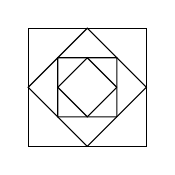
\begin{tikzpicture}
\pgfmathsetmacro{\k}{1.5}
\draw(0,0)--++(\k,0)coordinate[pos=0.5](a)--++(0,\k)coordinate[pos=0.5](b)--++(-\k,0)coordinate[pos=0.5](c)--++(0,-\k)coordinate[pos=0.5](d);
\draw(a)--(b)coordinate[pos=0.5](aa)--(c)coordinate[pos=0.5](bb)--(d)coordinate[pos=0.5](cc)--(a)coordinate[pos=0.5](dd);
\draw(aa)--(bb)coordinate[pos=0.5](aaa)--(cc)coordinate[pos=0.5](bbb)--(dd)coordinate[pos=0.5](ccc)--(aa)coordinate[pos=0.5](ddd);
\draw(aaa)--(bbb)coordinate[pos=0.5](aaaa)--(ccc)coordinate[pos=0.5](bbbb)--(ddd)coordinate[pos=0.5](cccc)--(aaa)coordinate[pos=0.5](dddd);
\end{tikzpicture}
\caption{چکور کے اندر چکور (سوال \حوالہ{سوال_تسلسل_چکور})}
\label{شکل_سوال_تسلسل_چکور}
\end{minipage}\hfill
\begin{minipage}{0.3\textwidth}
\centering
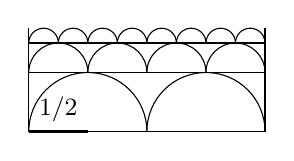
\begin{tikzpicture}[font=\small]
\pgfmathsetmacro{\k}{0.75}
\draw(0,\k+\k/2+\k/4)--(0,0)--(0,0)--(4*\k,0)--(4*\k,\k+\k/2+\k/4);
\draw(0,\k)--++(4*\k,0);
\draw(0,\k+\k/2)--++(4*\k,0);
\draw([shift={(0:\k)}]\k,0) arc (0:180:\k);
\draw([shift={(0:\k)}]3*\k,0) arc (0:180:\k);
\foreach \x in {1,3,5,7}{\draw([shift={(0:\k/2)}]\x*\k/2,\k) arc (0:180:\k/2);}
\foreach \x in {1,3,5,7,9,11,13,15}{\draw([shift={(0:\k/4)}]\x*\k/4,\k+\k/2) arc (0:180:\k/4);}
\draw[thick](0,0)--(\k,0)node[pos=0.5,above]{$1/2$};
\end{tikzpicture}
\caption{نصف دائروں کی قطاریں (سوال \حوالہ{سوال_تسلسل_نصف_دائرے})}
\label{شکل_سوال_تسلسل_نصف_دائرے}
\end{minipage}\hfill
\begin{minipage}{0.3\textwidth}
\centering
\begin{tikzpicture}[font=\scriptsize]
\pgfmathsetmacro{\k}{1.75}
\draw(\k+\k/2,\k/2)--++(0,\k/6+\k/7);
\draw(0,0) rectangle (2*\k,\k);
\draw(\k/2,0)node[below]{$1$}  (0,\k/2)node[left]{$1$} (\k+\k/4,0)node[below]{$\tfrac{1}{2}$} (\k+\k/2+\k/8,0)node[below]{$\tfrac{1}{4}$};
\draw(\k,0)--++(0,\k);
\draw[dashed](\k+\k/2,\k/4+\k/5+\k/6+\k/7)--(\k+\k/2,\k);
\draw[dashed](\k+\k/2+\k/4,\k/4)--(\k+\k/2+\k/4,\k);
\draw(\k,\k/2)--++(\k/2,0)--++(0,-\k/2);
\draw(\k+\k/3,\k/2)--++(0,\k/3)--++(-\k/3,0);
\draw(\k/2,\k/2)node[]{$1$};
\draw(\k+\k/4,\k/4)node[]{$\tfrac{1}{2^2}$};
\draw(\k+\k/6,\k/2+\k/6)node[]{$\tfrac{1}{3^2}$};
\draw(\k+\k/2+\k/4,0)--++(0,\k/4)--++(-\k/4,0);
\draw(\k+\k/2+\k/5,\k/4)--++(0,\k/5)--++(-\k/5,0);
\draw(\k+\k/2+\k/6,\k/4+\k/5)--++(0,\k/6)--++(-\k/6,0);
\draw(\k+\k/2+\k/7,\k/4+\k/5+\k/6)--++(0,\k/7)--++(-\k/7,0);
\draw(\k+\k/2+\k/8,\k/8)node[]{$\tfrac{1}{4^2}$};
\draw(\k+\k/2+\k/10,\k/4+\k/10)node[]{$\tfrac{1}{5^2}$};
\draw(\k+\k/2,\k/4+\k/5)node[pin=45:{$\tfrac{1}{6^2}$}]{};
\draw(\k+\k/2+\k/4+\k/8,0)node[below]{$\cdots$};
\draw(\k+\k/2+\k/4+\k/8,\k/2)node[]{$\cdots$};
\end{tikzpicture}
\caption{رقبوں کا مجموعہ \عددی{2} سے کم ہے (سوال \حوالہ{سوال_تسلسل_رقبہ_دو})}
\label{شکل_سوال_تسلسل_رقبہ_دو}
\end{minipage}
\end{figure}
%====================
\ابتدا{سوال}\شناخت{سوال_تسلسل_نصف_دائرے}
نصف دائروں کی صفوں کو شکل \حوالہ{شکل_سوال_تسلسل_نصف_دائرے} میں دکھایا گیا ہے جہاں نچلی صف میں رداس \عددی{\tfrac{1}{2}} ہے۔ \عددی{n} ویں صف میں نصف دائروں کی تعداد \عددی{2^n}  اور رداس \عددی{1/2^n} ہو گا۔ تمام نصف دائروں کے رقبوں کا مجموعہ تلاش کریں۔
\انتہا{سوال}
%=========================
\ابتدا{سوال}
متناہی رقبہ گھیرنے والی ہلگے ون کوچ برفانی روئی (صفحہ\حوالہصفحہ{حصہ_تفرق_برف_کی_روئی})  کی لمبائی لامتناہی ہوتی ہے۔ اس حقیقت کو سمجھنے کی خاطر فرض کریں ہم ضلع \عددی{1} کی مساوی الاضلاع مثلث سے شروع کرتے ہیں۔
\begin{enumerate}[a.]
\item
\عددی{n} ویں منحنی \عددی{C_n} کی لمبائی \عددی{L_n} تلاش کر کے دکھائیں کہ \عددی{\lim_{n\to \infty}L_n=\infty}  ہو گا۔
\item
\عددی{C_n} کا رقبہ \عددی{S_n} تلاش کر کے \عددی{\lim_{n\to\infty}S_n} معلوم کریں۔
\end{enumerate}
جواب:\quad
(الف) \عددی{3(\tfrac{4}{3})^{n-1}}، (ب) \عددی{A_n=A+\tfrac{1}{3}A+\tfrac{1}{3}(\tfrac{4}{9})A+\cdots+\tfrac{1}{3}(\tfrac{4}{9})^{n-2}A}،\\
  \عددی{\lim_{n\to\infty}A_n=\tfrac{2\sqrt{3}}{5}}
\انتہا{سوال}
%=========================
\ابتدا{سوال}\شناخت{سوال_تسلسل_رقبہ_دو}
ہم اس حقیقت کی غیر رسمی ثبوت کہ \عددی{\sum_{n=1}^{\infty}\tfrac{1}{n^2}} کی قیمت \عددی{2} سے کم ہے شکل \حوالہ{شکل_سوال_تسلسل_رقبہ_دو} کی مدد سے پیش کرتے ہیں۔ آپ کو کیا نظر آتا ہے؟
\انتہا{سوال}
%========================

\حصہ{غیر منفی اجزاء والے تسلسل کا تکملی پرکھ}
ہم تسلسل \عددی{\sum a_n} کے بارے میں دو سوالات کرتے ہیں:
\begin{enumerate}[a.]
\item
کیا یہ تسلسل مرتکز ہے؟
\item
اگر تسلسل مرتکز ہو تب اس کا مجموعہ کیا ہے؟
\end{enumerate}

اس باب کا باقی بیشتر حصہ پہلے سوال کا جواب دے گا۔ حقیقتاً دوسرا سوال بھی اتنا ہی اہم ہے اور ہم اس پر بعد میں غور کریں گے۔

اس حصہ میں اور اگلے دو حصوں میں ایسے تسلسل پر غور کیا جائے گا جن میں منفی اجزاء نہیں پائے جاتے ہوں۔ اس شرط کی بنا ان تسلسل کے جزوی مجموعے غیر گھٹتے ترتیبات دیتے ہیں اور وہ غیر گھٹتے ترتیبات جو  اوپر سے محدود ہوں ہر صورت مرتکز ہوتے ہیں (مسئلہ \حوالہ{مسئلہ_تسلسل_غیر_گھٹتا_تسلسل})۔ یہ دکھانے کی خاطر کہ ایک غیر منفی اجزاء والا تسلسل مرتکز ہے، ہمیں صرف اتنا دکھانا ہو گا کہ اس تسلسل کے جزوی مجموعے اوپر سے محدود ہیں۔

ابتدا میں یوں معلوم ہوتا ہے جیسے اس ترکیب سے ارتکاز کی تصدیق کرنے کے باوجود تسلسل کا مجموعہ نہ جاننا ایک عیب ہے۔ کیا بہتر ہوتا کہ ہم جزوی مجموعوں کے کلیات سے تسلسل کا مجموعہ بلا واسطہ تلاش کرتے۔ حقیقت میں ہمیں عموماً جزوی مجموعوں کے کلیات معلوم نہیں ہوں گے  اور اسی بنا ہمیں دو قدمی طریقہ کار استعمال کرنا ہو گا جہاں پہلے قدم میں تسلسل کا ارتکاز جانا جاتا ہے اور دوسرے قدم میں مجموعے کی تخمینی قیمت تلاش کی جاتی ہے۔ 

\جزوحصہء{غیر گھٹتے جزوی مجموعے}
فرض کریں کہ تمام \عددی{n} کے لئے \عددی{a_n\ge 0} ہو اور \عددی{\sum_{n=1}^{\infty}a_n} لامتناہی تسلسل ہو۔
 تب چونکہ \عددی{s_{n+1}=s_n+a_n} ہے لہٰذا ہر جزوی مجموعہ گزشتہ جزوی مجموعے سے بڑا یا اس کے برابر ہو گا:
\begin{align*}
s_1\le s_2\le s_3\le \cdots\le s_n\le s_{n+1}\le \cdots
\end{align*}
اب جزوی مجموعے غیر گھٹتا ترتیب بناتے ہیں اور مسئلہ \حوالہ{مسئلہ_تسلسل_غیر_گھٹتا_تسلسل} کے تحت یہ تسلسل صرف اور صرف اس صورت مرتکز ہو گا جب اس کے جزوی مجموعات اوپر سے محدود ہوں۔

\ابتدا{ضمنی نتیجہ}\شناخت{ضمنی_تسلسل_نتیجہ_الف} برائے مسئلہ \حوالہ{مسئلہ_تسلسل_غیر_گھٹتا_تسلسل}
غیر منفی اجزاء کا تسلسل \عددی{\sum_{n=1}^{\infty}a_n} صرف اور صرف اس صورت مرتکز ہو گا جب اس کے جزوی مجموعات اوپر سے محدود ہوں۔
\انتہا{ضمنی نتیجہ}
%=========================

\ابتدا{مثال}\ترچھا{ہارمونی تسلسل}\\
درج ذیل تسلسل کو \اصطلاح{ہارمونی تسلسل}\فرہنگ{تسلسل!ہارمونی}\حاشیہب{harmonic series}\فرہنگ{series!harmonic} کہتے ہیں۔
\begin{align*}
\sum_{n=1}^{\infty}\frac{1}{n}=1+\frac{1}{2}+\frac{1}{3}+\cdots+\frac{1}{n}+\cdots
\end{align*}
اس کے جزوی مجموعوں کی کوئی بالائی حد بندی نہیں پائی جاتی ہے لہٰذا یہ  مرتکز  تسلسل ہے۔ اس حقیقت کو جاننے کی خاطر ہم اجزاء کے گروہ بناتے ہیں۔
\begin{align*}
1+\frac{1}{2}+\underbrace{\big(\frac{1}{3}+\frac{1}{4}\big)}_{>\tfrac{2}{4}=\tfrac{1}{2}}+\underbrace{\big(\frac{1}{5}+\frac{1}{6}+\frac{1}{7}+\frac{1}{8}\big)}_{>\tfrac{4}{8}=\tfrac{1}{2}}+\underbrace{\big(\frac{1}{9}+\frac{1}{10}+\cdots+\frac{1}{16}\big)}_{>\tfrac{8}{16}=\tfrac{1}{2}}+\cdots
\end{align*}
پہلے دو اجزاء کا مجموعہ \عددی{1.5} ہے۔اگلے دو اجزاء کا مجموعہ \عددی{\tfrac{1}{3}+\tfrac{1}{4}} ہے جو \عددی{\tfrac{1}{4}+\tfrac{1}{4}=\tfrac{1}{2}} سے بڑا ہے۔ اگلے چار اجزاء کا مجموعہ \عددی{\tfrac{1}{5}+\tfrac{1}{6}+\tfrac{1}{7}+\tfrac{1}{8}} ہے جو \عددی{\tfrac{1}{8}+\tfrac{1}{8}+\tfrac{1}{8}+\tfrac{1}{8}=\tfrac{1}{2}} سے بڑا ہے۔ اگلے آٹھ اجزاء کا مجموعہ
 \عددی{\tfrac{1}{9}+\tfrac{1}{10}+\tfrac{1}{11}+\tfrac{1}{12}+\tfrac{1}{13}+\tfrac{1}{14}+\tfrac{1}{15}+\tfrac{1}{16}} ہے جو  \عددی{\tfrac{1}{16}+\tfrac{1}{16}+\tfrac{1}{16}+\tfrac{1}{16}+\tfrac{1}{16}+\tfrac{1}{16}+\tfrac{1}{16}+\tfrac{1}{16}=\tfrac{1}{2}} سے بڑا ہے۔ اسی طرح اگلے سولہ اجزاء کا مجموعہ بھی \عددی{\tfrac{1}{2}} سے بڑا ہو گا، وغیرہ وغیرہ۔ یوں جزو \عددی{\tfrac{1}{2^{n+1}}} پر اختتام پذیر  \عددی{2^n} اجزاء کا مجموعہ \عددی{\tfrac{2^n}{2^{n+1}}=\tfrac{1}{2}} سے بڑا ہو گا۔جزوی مجموعات کی ترتیب اوپر سے محدود نہیں ہے: اگر \عددی{n=2^k} ہو تب جزوی مجموعہ \عددی{s_n} کی قیمت \عددی{\tfrac{k}{2}} سے بڑی ہو گی۔ ہارمونی تسلسل منفرج ہے۔
\انتہا{مثال}
%===========================

دھیان رہے کہ ہارمونی تسلسل کا \عددی{n} واں جزو \عددی{\tfrac{1}{n}} ہے جو \عددی{0} پر مرتکز ہے لیکن ہارمونی تسلسل منفرج ہے۔یوں ہارمونی تسلسل کے انفراج کو دریافت کرنے میں انفراج کا \عددی{n} ویں جزو پرکھ  نا کام  ہوتا ہے۔

\جزوحصہء{تکملی پرکھ}
ہم ہارمونی تسلسل سے تعلق رکھنے والے ایک تسلسل، جس کا \عددی{n} واں جزو \عددی{\tfrac{1}{n^2}} ہے، کو استعمال کرتے ہوئے تکملی پرکھ کو متعارف کرتے ہیں۔

\ابتدا{مثال}\شناخت{مثال_تسلسل_مرتکز_تسلسل_موازنہ_تکمل}
کیا درج ذیل تسلسل مرتکز ہے؟
\begin{align*}
\sum_{n=1}^{\infty}\frac{1}{n^2}=1+\frac{1}{4}+\frac{1}{9}+\frac{1}{16}+\cdots+\frac{1}{n^2}+\cdots
\end{align*}
حل:\quad
ہم \عددی{\int_1^{\infty}\tfrac{\dif x}{x^2}} کے ساتھ موازنہ کرتے ہوئے \عددی{\sum_{n=1}^{\infty}\tfrac{1}{n^2}} کی ارتکاز دریافت کرتے ہیں۔ موازنہ کرنے کی خاطر ہم تسلسل کے اجزاء کو تفاعل \عددی{f(x)=\tfrac{1}{x^2}} کی قیمتیں تصور کرتے ہیں اور ان قیمتوں کو منحنی \عددی{y=\tfrac{1}{x^2}} کے نیچے مستطیل رقبے تصور کرتے ہیں۔

جیسا شکل \حوالہ{شکل_مثال_تسلسل_مرتکز_تسلسل_موازنہ_تکمل} میں دکھایا گیا ہے درج ذیل ہو گا۔
\begin{align*}
s_n&=\frac{1}{1^2}+\frac{1}{2^2}+\frac{1}{3^2}+\cdots+\frac{1}{n^2}\\
&=f(1)+f(2)+f(3)+\cdots+f(n)\\
&<f(1)+\int_1^{n}\frac{1}{x^2}\dif x\\
&<1+\int_1^{\infty}\frac{1}{x^2}\dif x\\
&<1+1=2&&\text{\RL{(مثال \حوالہ{مثال_طریقہ_منحنی_کے_نیچے_رقبہ_متناہی_یا_نہیں})}}
\end{align*}
یوں \عددی{\sum_{n=1}^{\infty}\tfrac{1}{n^2}} کے جزوی مجموعات اوپر سے (\عددی{2} تک) محدود ہیں لہٰذا یہ تسلسل مرتکز ہو گا۔  اس تسلسل کا مجموعہ درحقیقت \عددی{\tfrac{\pi^2}{6}\approx 1.64493} ہے۔
\انتہا{مثال}
%=======================
\begin{figure}
\centering
\begin{tikzpicture}[font=\small,declare function={f(\x)=1/(\x^2);}]
\begin{axis}[clip=false,small,axis lines=middle,xlabel={$x$},ylabel={$y$},xlabel style={at={(current axis.right of origin)},anchor=west},ylabel style={at={(current axis.above origin)},anchor=south},xmin=0,ymin=0,ytick={\empty},xtick={1,2,3,4,7,8},xticklabels={$1$,$2$,$3$,$4$,$n-1$,$n$}]
\addplot[smooth,domain=0.9:9]{f(x)};
\draw(0,{f(1)})--(1,{f(1)})node[right]{$(1,f(1))$}--(1,0);
\draw(1,{f(2)})--(2,{f(2)})node[pin={[pin distance=1cm]70:{$(2,f(2))$}}]{}--(2,0);
\draw(2,{f(3)})--(3,{f(3)})node[pin={[pin distance=1cm]50:{$(3,f(3))$}}]{}--(3,0);
\draw(3,{f(4)})--(4,{f(4)})--(4,0);
\draw(1/2,{1/2*f(1)})node[]{$\tfrac{1}{1^2}$};
\draw(1+1/2,{1/2*f(2)})node[]{$\tfrac{1}{2^2}$};
\draw(2.2,{1/3*f(3)})node[pin=60:{$\tfrac{1}{3^2}$}]{};
\draw(3.2,{1/4*f(4)})node[pin=30:{$\tfrac{1}{4^2}$}]{};
\draw(8,{f(8)})node[pin=45:{$(n,f(n))$}]{};
\draw(7.5,{0})node[pin=70:{$\tfrac{1}{n^2}$}]{};
\draw(7,{f(1)})node[]{$f(x)=\frac{1}{x^2}$};
\end{axis}
\end{tikzpicture}
\caption{رقبہ کا موازنہ (مثال \حوالہ{مثال_تسلسل_مرتکز_تسلسل_موازنہ_تکمل})}
\label{شکل_مثال_تسلسل_مرتکز_تسلسل_موازنہ_تکمل}
\end{figure}

\ابتدا{پرکھ}\موٹا{تکملی پرکھ}\\
فرض کریں \عددی{\{a_n\}} مثبت اجزاء کی ترتیب ہے۔ مزید فرض کریں کہ \عددی{a_n=f(n)} ہے جہاں تمام \عددی{x\ge N} کے لئے ( \عددی{N} مثبت عدد صحیح ہے)  متغیر \عددی{x} کا \عددی{f}  استمراری، مثبت اور گھٹتا تفاعل ہے۔ تب تسلسل \عددی{\sum_{n=N}^{\infty}a_n} اور تکمل \عددی{\int_N^{\infty}f(x)\dif  x} دونوں مرتکز یا دونوں منفرج ہوں گے۔
\انتہا{پرکھ}
%==================
\ابتدا{ثبوت پرکھ}
ہم \عددی{N=1} کے لئے پہلے اس پرکھ کو ثابت کرتے ہیں۔ عمومی \عددی{N} کے لئے ثبوت اسی طرح کا ہے۔ 

ہم اس مفروضہ سے شروع کرتے ہیں کہ تمام \عددی{n} کے لئے \عددی{f} گھٹتا تفاعل  اور \عددی{f(n)=a_n} ہیں۔ یوں شکل \حوالہ{شکل_تسلسل_تکملی_پرکھ_ثبوت}-الف میں وہ مستطیل جن کے رقبے \عددی{a_1,a_2,\cdots,a_n}  ہیں کا مجموعی رقبہ، \عددی{x=1} تا \عددی{x=n+1} ترسیم \عددی{y=f(x)} کے نیچے رقبہ سے زیادہ ہے یعنی:
\begin{align*}
\int_1^{n+1}f(x)\dif x\le a_1+a_2+\cdots+a_n
\end{align*} 
شکل \حوالہ{شکل_تسلسل_تکملی_پرکھ_ثبوت}-ب میں مستطیلوں کو ہر نقطہ کے بائیں جانب بنایا گیا ہے۔ اگر ہم وقتی طور پر پہلی مستطیل، جس کا رقبہ \عددی{a_1} ہے، کو نظر انداز کریں تب درج ذیل ہو گا۔
\begin{align*}
a_2+a_3+\cdots+a_n\le \int_1^nf(x)\dif x
\end{align*}
اگر ہم \عددی{a_1} کو بھی شامل کریں تب درج ذیل لکھا جا سکتا ہے۔
\begin{align*}
a_1+a_2+a_3+\cdots+a_n\le a_1+\int_1^nf(x)\dif x
\end{align*}
ان نتائج سے 
\begin{align}\label{مساوات_تسلسل_عدم_مساواتیں}
\int_1^{n+1}f(x)\dif x\le a_1+a_2+\cdots+a_n\le  a_1+\int_1^nf(x)\dif x
\end{align}
حاصل ہوتا ہے۔ اگر \عددی{\int_1^{\infty}f(x)\dif x} متناہی ہو تب دائیں عدم مساوات کے تحت \عددی{\sum a_n} متناہی ہو گا۔  اگر \عددی{\int_1^{\infty}f(x)\dif x} لامتناہی ہو تب بائیں عدم مساوات کے تحت \عددی{\sum a_n} لامتناہی ہو گا۔ 

یوں تسلسل اور تکمل دونوں مرتکز یا دونوں منفرج ہوں گے۔
\انتہا{ثبوت پرکھ}
%=======================
\begin{figure}
\centering
\begin{subfigure}{0.45\textwidth}
\centering
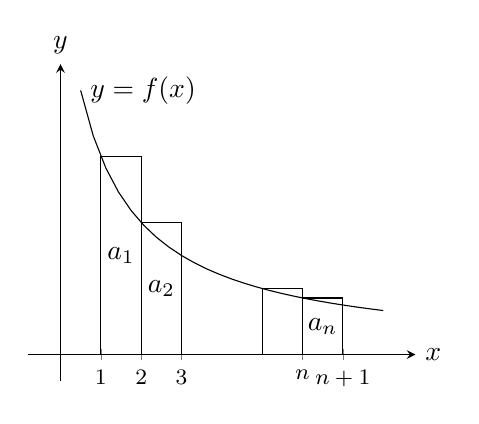
\begin{tikzpicture}[declare function={f(\x)=1/(1+\x);}]
\begin{axis}[small,axis lines=middle,xlabel={$x$},ylabel={$y$},xmin=0,ymin=0,enlargelimits=true,xtick={1,2,3,6,7},xticklabels={$1$,$2$,$3$,$n$,$n+1$},ytick={\empty},xlabel style={at={(current axis.right of origin)},anchor=west},ylabel style={at={(current axis.above origin)},anchor=south}]
\addplot[domain=0.5:8]{f(x)}node[pos=0,right]{$y=f(x)$};
\draw(1,0)--(1,{f(1)})--(2,{f(1)})--(2,{f(2)});
\draw(2,0)--(2,{f(2)})--(3,{f(2)})--(3,0);
\draw(5,0)--(5,{f(5)})--(6,{f(5)})--(6,{f(6)});
\draw(6,0)--(6,{f(6)})--(7,{f(6)})--(7,0);
\draw(1.5,{1/2*f(1)})node[]{$a_1$};
\draw(2.5,{1/2*f(2)})node[]{$a_2$};
\draw(6.5,{1/2*f(6)})node[]{$a_n$};
\end{axis}
\end{tikzpicture}
\caption{}
\end{subfigure}\hfill
\begin{subfigure}{0.45\textwidth}
\centering
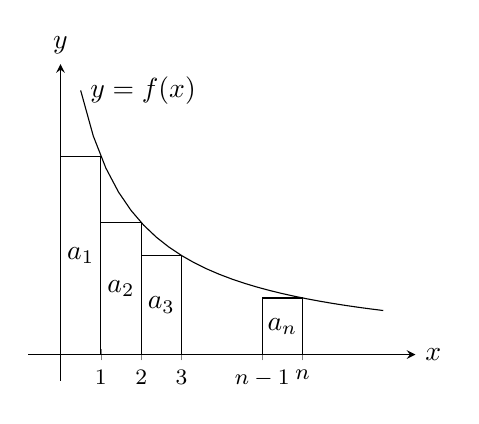
\begin{tikzpicture}[declare function={f(\x)=1/(1+\x);}]
\begin{axis}[small,axis lines=middle,xlabel={$x$},ylabel={$y$},xmin=0,ymin=0,enlargelimits=true,xtick={1,2,3,5,6},xticklabels={$1$,$2$,$3$,$n-1$,$n$},ytick={\empty},xlabel style={at={(current axis.right of origin)},anchor=west},ylabel style={at={(current axis.above origin)},anchor=south}]
\addplot[domain=0.5:8]{f(x)}node[pos=0,right]{$y=f(x)$};
\draw(0,{f(1)})--(1,{f(1)})--(1,0);
\draw(1,{f(2)})--(2,{f(2)})--(2,0);
\draw(2,{f(3)})--(3,{f(3)})--(3,0);
\draw(5,0)--(5,{f(6)})--(6,{f(6)})--(6,0);
\draw(0.5,{1/2*f(1)})node[]{$a_1$};
\draw(1.5,{1/2*f(2)})node[]{$a_2$};
\draw(2.5,{1/2*f(3)})node[]{$a_3$};
\draw(5.5,{1/2*f(6)})node[]{$a_n$};
\end{axis}
\end{tikzpicture}
\caption{}
\end{subfigure}
\caption{تکملی پرکھ کے تحت تسلسل $\sum_{n=1}^{\infty}a_n$ اور تکمل $\int_1^{\infty}f(x)\dif x$ دونوں مرتکز یا دونوں منفرج ہوں گے۔}
\label{شکل_تسلسل_تکملی_پرکھ_ثبوت}
\end{figure}

%====================
دھیان رہے کہ ارتکاز کی صورت میں تکمل اور تسلسل کی قیمتیں مختلف ہو سکتی ہیں جیسا مثال \حوالہ{مثال_تسلسل_مرتکز_تسلسل_موازنہ_تکمل} میں دیکھا گیا جہاں \عددی{\sum_{n=1}^{\infty}\tfrac{1}{n^2}=\tfrac{\pi^2}{6}} اور \عددی{\int_1^{\infty}\tfrac{1}{x^2}\dif x=1} تھے۔

\ابتدا{مثال}
دکھائیں کہ \عددی{p} تسلسل
\begin{align}
\sum_{n=1}^{\infty}\frac{1}{n^p}=\frac{1}{1^p}+\frac{1}{2^p}+\frac{1}{3^p}+\cdots+\frac{1}{n^p}+\cdots
\end{align}
جہاں \عددی{p} حقیقی مستقل ہے، \عددی{p>1} کی صورت میں مرتکز جبکہ \عددی{p\le 1} کی صورت میں منفرج ہو گا۔

حل:\quad
اگر \عددی{p>1} ہو تب \عددی{f(x)=\tfrac{1}{x^p}} متغیر \عددی{x} کا مثبت گھٹتا تفاعل ہو گا۔ اب چونکہ
\begin{align*}
\int_1^{\infty}\frac{1}{x^p}\dif x&=\int_1^{\infty}x^{-p}\dif x=\lim_{b\to\infty}\big[\frac{x^{-p+1}}{-p+1}\big]_1^b\\
&=\frac{1}{1-p}\lim_{b\to\infty}(\frac{1}{b^{p-1}}-1)\\
&=\frac{1}{1-p}(0-1)=\frac{1}{p-1}
\end{align*}
ہے لہٰذا تکملی پرکھ کے تحت یہ تسلسل مرتکز ہو گا۔

اگر \عددی{p<1}ہو تب \عددی{1-p>0} ہو گا لہٰذا درج ذیل لکھا جا سکتا ہے۔
\begin{align*}
\int_1^{\infty}\frac{1}{x^p}\dif x=\frac{1}{1-p}\lim_{b\to\infty}(b^{1-p}-1)=\infty
\end{align*}
تکملی پرکھ کے تحت یہ تسلسل منفرج ہو گا۔

اگر \عددی{p=1} ہو تب درج ذیل منفرج (ہارمونی) تسلسل پایا جائے گا۔
\begin{align*}
1+\frac{1}{2}+\frac{1}{3}+\cdots+\frac{1}{n}+\cdots
\end{align*} 
یوں \عددی{p>1} لے ارتکاز  لیکن \عددی{p<1} اور \عددی{p=0} کے لئے انفراج پایا جاتا ہے۔
\انتہا{مثال}
%=====================
\حصہء{سوالات}
\موٹا{ارتکاز اور انفراج کی معلومات}\\
سوال \حوالہ{سوال_تسلسل_ارتکاز_یا_انفراج_الف} تا سوال \حوالہ{سوال_تسلسل_ارتکاز_یا_انفراج_ب} میں کون سا تسلسل مرتکز اور کان سا تسلسل منفرج ہے؟ اپنے جواب کی وجہ پیش کریں۔(جوابات دیکھتے ہوئے یاد رہے کہ تسلسل کی ارتکاز یا انفراج جاننے کے کئی طریقے ہو سکتے ہیں)

\ابتدا{سوال}\شناخت{سوال_تسلسل_ارتکاز_یا_انفراج_الف}
$\sum\limits_{n=1}^{\infty}\frac{1}{10^n}$\\
جواب:\quad
مرتکز؛ ہندسی تسلسل، \عددی{r=\tfrac{1}{10}<1}
\انتہا{سوال}
%==========================
\ابتدا{سوال}
$\sum\limits_{n=1}^{\infty}e^{-n}$
\انتہا{سوال}
%==========================
\ابتدا{سوال}
$\sum\limits_{n=1}^{\infty}\frac{n}{n+1}$\\
جواب:\quad
منفرج؛ \عددی{\lim_{n\to\infty}\tfrac{n}{n+1}=1\ne 0} 
\انتہا{سوال}
%==========================
\ابتدا{سوال}
$\sum\limits_{n=1}^{\infty}\frac{5}{n+1}$
\انتہا{سوال}
%==========================
\ابتدا{سوال}
$\sum\limits_{n=1}^{\infty}\frac{3}{\sqrt{n}}$\\
جواب:\quad
منفرج؛ \عددی{p} تسلسل، \عددی{p<1}
\انتہا{سوال}
%==========================
\ابتدا{سوال}
$\sum\limits_{n=1}^{\infty}\frac{-2}{n\sqrt{n}}$
\انتہا{سوال}
%==========================
\ابتدا{سوال}
$\sum\limits_{n=1}^{\infty}-\frac{1}{8^n}$\\
جواب:\quad
مرتکز؛ ہندسی تسلسل، \عددی{r=\tfrac{1}{8}<1}
\انتہا{سوال}
%==========================
\ابتدا{سوال}
$\sum\limits_{n=1}^{\infty}-\frac{8}{n}$
\انتہا{سوال}
%==========================
\ابتدا{سوال}
$\sum\limits_{n=2}^{\infty}\frac{\ln n}{n}$\\
جواب:\quad
منفرج؛ تکملی پرکھ
\انتہا{سوال}
%==========================
\ابتدا{سوال}
$\sum\limits_{n=2}^{\infty}\frac{\ln n}{\sqrt{n}}$
\انتہا{سوال}
%==========================
\ابتدا{سوال}
$\sum\limits_{n=1}^{\infty}\frac{2^n}{3^n}$\\
جواب:\quad
مرتکز؛ ہندسی تسلسل، \عددی{r=\tfrac{2}{3}<1}
\انتہا{سوال}
%==========================
\ابتدا{سوال}
$\sum\limits_{n=1}^{\infty}\frac{5^n}{4^n+3}$
\انتہا{سوال}
%==========================
\ابتدا{سوال}
$\sum\limits_{n=0}^{\infty}\frac{-2}{n+1}$\\
جواب:\quad
منفرج؛ تکملی پرکھ
\انتہا{سوال}
%==========================
\ابتدا{سوال}
$\sum\limits_{n=1}^{\infty}\frac{1}{2n-1}$
\انتہا{سوال}
%==========================
\ابتدا{سوال}
$\sum\limits_{n=1}^{\infty}\frac{2^n}{n+1}$\\
جواب:\quad
منفرج؛ \عددی{\lim_{n\to\infty}\tfrac{2^n}{n+1}\ne 0}
\انتہا{سوال}
%==========================
\ابتدا{سوال}
$\sum\limits_{n=1}^{\infty}\frac{1}{\sqrt{n}(\sqrt{n}+1)}$
\انتہا{سوال}
%==========================
\ابتدا{سوال}
$\sum\limits_{n=2}^{\infty}\frac{\sqrt{n}}{\ln n}$\\
جواب:\quad
منفرج؛ \عددی{\lim_{n\to\infty}(\tfrac{\sqrt{n}}{\ln n})\ne 0}
\انتہا{سوال}
%==========================
\ابتدا{سوال}
$\sum\limits_{n=1}^{\infty}\big(1+\frac{1}{n}\big)^n$
\انتہا{سوال}
%==========================
\ابتدا{سوال}
$\sum\limits_{n=1}^{\infty}\frac{1}{(\ln 2)^n}$\\
جواب:\quad
منفرج؛ ہندسی تسلسل، \عددی{r=\tfrac{1}{\ln2}>1}
\انتہا{سوال}
%==========================
\ابتدا{سوال}
$\sum\limits_{n=1}^{\infty}\frac{1}{(\ln 3)^n}$
\انتہا{سوال}
%==========================
\ابتدا{سوال}
$\sum\limits_{n=3}^{\infty}\frac{1/n}{(\ln n)\sqrt{\ln^2 n-1}}$\\
جواب:\quad
مرتکز؛  تکملی پرکھ
\انتہا{سوال}
%==========================
\ابتدا{سوال}
$\sum\limits_{n=1}^{\infty}\frac{1}{n(1+\ln^2n)}$
\انتہا{سوال}
%==========================
\ابتدا{سوال}
$\sum\limits_{n=1}^{\infty}n\sin\frac{1}{n}$\\
جواب:\quad
منفرج؛ \عددی{n} واں جزو پرکھ
\انتہا{سوال}
%==========================
\ابتدا{سوال}
$\sum\limits_{n=1}^{\infty}n\tan \frac{1}{n}$
\انتہا{سوال}
%==========================
\ابتدا{سوال}
$\sum\limits_{n=1}^{\infty}\frac{e^n}{1+e^{2n}}$\\
جواب:\quad
مرتکز؛ تکملی پرکھ
\انتہا{سوال}
%==========================
\ابتدا{سوال}
$\sum\limits_{n=1}^{\infty}\frac{2}{1+e^n}$
\انتہا{سوال}
%==========================
\ابتدا{سوال}
$\sum\limits_{n=1}^{\infty}\frac{8\tan^{-1}n}{1+n^2}$\\
جواب:\quad
مرتکز؛ تکملی پرکھ
\انتہا{سوال}
%==========================
\ابتدا{سوال}
$\sum\limits_{n=1}^{\infty}\frac{n}{n^2+1}$
\انتہا{سوال}
%==========================
\ابتدا{سوال}
$\sum\limits_{n=1}^{\infty}\sech n$\\
جواب:\quad
مرتکز؛ تکملی پرکھ
\انتہا{سوال}
%==========================
\ابتدا{سوال}\شناخت{سوال_تسلسل_ارتکاز_یا_انفراج_ب}
$\sum\limits_{n=1}^{\infty}\sech^2 n$
\انتہا{سوال}
%==========================
\موٹا{نظریہ اور مثالیں}\\
سوال \حوالہ{سوال_تسلسل_ارتکاز_کا_اے_الف} اور سوال \حوالہ{سوال_تسلسل_ارتکاز_کا_اے_ب} میں اگر کسی \عددی{a} کے لئے تسلسل مرتکز ہو تب \عددی{a} تلاش کریں۔ 

\ابتدا{سوال}\شناخت{سوال_تسلسل_ارتکاز_کا_اے_الف}
$\sum\limits_{n=1}^{\infty}\big(\frac{a}{n+2}-\frac{1}{n+4}\big)$\\
جواب:\quad
(الف) \عددی{a=1}
\انتہا{سوال}
%========================
\ابتدا{سوال}\شناخت{سوال_تسلسل_ارتکاز_کا_اے_ب}
$\sum\limits_{n=3}^{\infty}\big(\frac{1}{n-1}-\frac{2a}{n+1}\big)$
\انتہا{سوال}
%========================
\ابتدا{سوال}
\begin{enumerate}[a.]
\item
شکل \حوالہ{شکل_مثال_تسلسل_مرتکز_تسلسل_موازنہ_تکمل} اور شکل \حوالہ{شکل_تسلسل_تکملی_پرکھ_ثبوت} کی طرز کے اشکال بنا کر دکھائیں کہ ہارمونی تسلسل کے جزوی مجموعات درج ذیل عدم مساواتوں کو مطمئن کرتے ہیں۔ 
\begin{align*}
\ln(n+1)&=\int_1^{n+1}\frac{1}{x}\dif x\le 1+\frac{1}{2}+\cdots+\frac{1}{n}\\
&\le 1+\int_1^n\frac{1}{x}\dif x=1+\ln n
\end{align*}
%
\item
ہارمونی تسلسل کی انفراج  تجرباتی طور نظر نہیں آتی ہے اگرچہ ہم جانتے ہیں کہ یہ تسلسل منفرج ہے۔ بس اس کے جزوی مجموعات بہت آہستہ بڑھتے ہیں۔یہ دیکھنے کی خاطر فرض کریں ہم \عددی{s_1=1} سے شروع کر کے ہر سیکنڈ ہارمونی تسلسل میں ایک جزو شامل کرتے ہیں۔کائنات کی ابتدا سے شروع کرتے ہوئے اب تک (تقریباً \عددی{13} ارب سال بعد) شامل اجزاء کا جزوی مجموعہ کیا ہو گا؟ (ایک سال میں \عددی{365} دن لیں۔)
\end{enumerate}
جواب:\quad
(ب) تقریباً \عددی{41.55}
\انتہا{سوال}
%==============
\ابتدا{سوال}
کیا \عددی{x} کی کسی قیمت کے لئے \عددی{\sum_{n=1}^{\infty}\tfrac{1}{nx}} مرتکز ہو گا؟ اپنے جواب کی وجہ پیش کریں۔
\انتہا{سوال}
%============================
\ابتدا{سوال}\شناخت{سوال_تسلسل_چھوٹا_منفرج_الف}
کیا یہ درست ہے کہ اگر \عددی{\sum_{n=1}^{\infty}a_n} مثبت اعداد کا منفرج تسلسل ہو تب تمام \عددی{n} کے لئے \عددی{b_n<a_n} کی صورت میں مثبت اعداد کا ایک تسلسل \عددی{\sum_{n=1}^{\infty}b_n} بھی منفرج ہو گا؟ کیا مثبت اعداد کا  "چھوٹے سے چھوٹا" منفرج تسلسل پایا جاتا ہے؟ اپنے جواب کی وجہ پیش کریں۔\\
جواب:\quad
درست ہے۔
\انتہا{سوال}
%=========================
\ابتدا{سوال}
کیا مثبت اعداد کا "بڑے سے بڑا" منفرج تسلسل پایا جاتا ہے (سوال \حوالہ{سوال_تسلسل_چھوٹا_منفرج_الف})؟
\انتہا{سوال}
%==========================
\ابتدا{سوال}\شناخت{سوال_تسلسل_کوشی_پرکھ_جمود}\ترچھا{کوشی پرکھ جمود}\\
کوشی پرکھ جمود کہتا ہے: فرض کریں \عددی{\{a_n\}} مثبت اجزاء کی غیر گھٹتی ترتیب ہے  (تمام \عددی{n} کے لئے \عددی{a_n\ge a_{n+1}})  جو \عددی{0} پر مرتکز ہے۔تب \عددی{\sum a_n} صرف اور صرف اس صورت مرتکز ہو گا جب \عددی{\sum 2^n a_{2^n}} مرتکز ہو۔ مثال کے طور پر \عددی{\sum \tfrac{1}{n}}  اس لئے منفرج  ہے کہ \عددی{\sum 2^n\cdot (\tfrac{1}{2^n})=\sum 1} منفرج ہے۔ دکھائیں کہ یہ پرکھ کیوں کام کرتا ہے۔
\انتہا{سوال}
%======================
\ابتدا{سوال}
کوشی پرکھ جمود (سوال \حوالہ{سوال_تسلسل_کوشی_پرکھ_جمود}) استعمال کرتے ہوئے دکھائیں کہ
\begin{enumerate}[a.]
\item
\عددی{\sum\limits_{n=2}^{\infty}\frac{1}{n\ln n}} منفرج ہے۔
\item
\عددی{p>1} کے لئے \عددی{\sum\limits_{n=1}^{\infty}\tfrac{1}{n^p}} مرتکز اور \عددی{p\le 1} کے لئے منفرج ہے۔
\end{enumerate}
\انتہا{سوال}
%=====================
\ابتدا{سوال}\شناخت{سوال_تسلسل_لوگارتھمی_پی_تسلسل}\ترچھا{لوگارتھمی \عددی{p} تسلسل}\\
\begin{enumerate}[a.]
\item
دکھائیں کہ صرف اور صرف \عددی{p>1} کے لئے  \عددی{\int_2^{\infty}\tfrac{\dif x}{x(\ln x)^p}} مرتکز ہو گا۔
\item
تسلسل \عددی{\sum_2^{\infty}\tfrac{1}{n(\ln n)^p}} کی ارتکاز پر جزو-الف کا کیا اثر ہو گا؟ اپنے جواب کی وجہ پیش کریں۔
\end{enumerate}
\انتہا{سوال}
%=====================
\ابتدا{سوال}
درج ذیل میں کون سے تسلسل مرتکز اور کون سے منفرج ہیں۔ سوال \حوالہ{سوال_تسلسل_لوگارتھمی_پی_تسلسل} کے نتائج بروئے کار لائیں۔ اپنے جواب کی وجہ پیش کریں۔
\begin{multicols}{4}
\begin{enumerate}[a.]
\item
$\sum\limits_{n=2}^{\infty}\frac{1}{n\ln n}$
\item
$\sum\limits_{n=2}^{\infty}\frac{1}{n(\ln n)^{1.01}}$
\item
$\sum\limits_{n=2}^{\infty}\frac{1}{n\ln (n^3)}$
\item
$\sum\limits_{n=2}^{\infty}\frac{1}{n(\ln n)^3}$
\end{enumerate}
\end{multicols}
\انتہا{سوال}
%======================
\ابتدا{سوال}\ترچھا{یولر مستقل}\\
ہم شکل \حوالہ{شکل_تسلسل_تکملی_پرکھ_ثبوت} کی طرح اشکال کو دیکھ کر ہمیں خیال آتا ہے کہ \عددی{n} بڑھانے سے  مجموعہ
\begin{align*}
1+\frac{1}{2}+\cdots+\frac{1}{n}
\end{align*}
 اور تکمل
\begin{align*}
\ln n=\int_1^n\frac{1}{x}\dif x
\end{align*}
کے فرق میں کمی کم ہوتی ہے۔اس خیال پر غور کی خاطر درج ذیل اقدام کریں۔
\begin{enumerate}[a.]
\item
عدم مساوات \حوالہ{مساوات_تسلسل_عدم_مساواتیں} میں \عددی{f(x)=\tfrac{1}{x}} لے کر 
\begin{align*}
\ln (n+1)\le 1+\frac{1}{2}+\cdots+\frac{1}{n}\le 1+\ln n
\end{align*}
یا 
\begin{align*}
0<\ln (n+1)-\ln n\le 1+\frac{1}{2}+\cdots+\frac{1}{n}-\ln n\le 1
\end{align*}

دکھائیں۔یوں درج ذیل ترتیب اوپر سے اور نیچے سے محدود ہو گی۔
\begin{align*}
a_n=1+\frac{1}{2}+\cdots+\frac{1}{n}-\ln n
\end{align*}
\item
درج ذیل دکھا کر دکھائیں کہ جز-الف میں ترتیب \عددی{\{a_n\}} گھٹتی ترتیب ہے۔
\begin{align*}
\frac{1}{n+1}<\int_n^{n+1}\frac{1}{x}\dif x=\ln (n+1)-\ln n
\end{align*} 
چونکہ اوپر اور نیچے سے محدود گھٹتی ترتیب مرتکز ہوتی ہے (سوال \حوالہ{سوال_تسلسل_غیر_بڑھتا_ترتیب})  لہٰذا جزو-الف میں اعداد \عددی{a_n} بھی مرتکز ہوں گے:
\begin{align*}
1+\frac{1}{2}+\cdots+\frac{1}{n}-\ln n\to \gamma
\end{align*}
عدد \عددی{\gamma} جس کو \اصطلاح{یولر مستقل}\فرہنگ{یولر!مستقل}\حاشیہب{Euler's constant}\فرہنگ{Euler's!constant} کہتے ہیں کی قیمت \عددی{0.5772\cdots} ہے۔ دیگر مخصوص اعداد مثلاً \عددی{\pi} اور \عددی{e} کے برعکس \عددی{\gamma} کو ظاہر کرنے کا کوئی دوسرا  سادہ کلیہ اب تک دریافت نہیں کیا گیا ہے۔
\end{enumerate}
\انتہا{سوال}
%====================
\ابتدا{سوال}
تکملی پرکھ استعمال کرتے ہوئے دکھائیں کہ \عددی{\sum_{n=0}^{\infty}e^{-n^2}} مرتکز ہے۔
\انتہا{سوال}
%====================

\حصہ{غیر منفی اجزاء کے تسلسل کے تقابلی پرکھ}
گزشتہ حصہ کے ضمنی نتیجہ \حوالہ{ضمنی_تسلسل_نتیجہ_الف} کی استعمال میں اصل سوال یہ  معلوم کرنا ہے کہ \عددی{s_n} اوپر سے محدود ہے۔ بعض اوقات ہم دکھا پاتے ہیں کہ چونکہ دیے گئے تسلسل کا ہر جزوی مجموعہ \عددی{s_n} کسی مرتکز تسلسل کے  مطابقتی جزوی مجموعہ سے کم ہے لہٰذا دیا گیا تسلسل مرتکز ہے۔

\ابتدا{مثال}\شناخت{مثال_تسلسل_پرکھ_موازنہ_استعمال}
درج ذیل تسلسل
\begin{align*}
\sum\limits_{n=0}^{\infty}\frac{1}{n!}=1+\frac{1}{1!}+\frac{1}{2!}+\frac{1}{3!}+\cdots
\end{align*}
 اس لئے مرتکز ہے کہ اس کے تمام اجزاء مثبت اور  درج ذیل تسلسل کے مطابقتی اجزاء سے کم ہیں۔
\begin{align*}
1+\sum_{n=0}^{\infty}\frac{1}{2^n}=1+1+\frac{1}{2}+\frac{1}{2^2}+\cdots
\end{align*}
آئیں دیکھتے ہیں کہ یہ تعلق \عددی{\sum_{n=0}^{\infty}\tfrac{1}{n!}}  کے جزوی مجموعات کو کیسے اوپر سے محدود بناتا ہے۔ درج ذیل فرض کر کے
\begin{align*}
s_n=1+\frac{1}{1!}+\frac{1}{2!}+\cdots+\frac{1}{n!}
\end{align*}
ہم دیکھتے ہیں کہ ہر \عددی{n} کے لئے
\begin{align*}
s_n\le 1+1+\frac{1}{2}+\frac{1}{2^2}+\cdots+\frac{1}{2^{n-1}}<1+\sum_{n=0}^{\infty}\frac{1}{2^n}=1+\frac{1}{1-(1/2)}=3
\end{align*}
ہو گا۔ یوں \عددی{\sum_{n=0}^{\infty}\tfrac{1}{n!}} کے تمام جزوی مجموعات \عددی{3} سے کم ہیں لہٰذا \عددی{\sum_{n=0}^{\infty}\tfrac{1}{n!}} مرتکز ہو گا۔

\عددی{\sum_{n=0}^{\infty}\tfrac{1}{n!}} کے جزوی مجموعات کی بالائی حد بندی \عددی{3} ہونے کا یہ مطلب نہیں کہ یہ تسلسل \عددی{3} پر مرتکز ہو گا۔ جیسا ہم آگے اس باب میں دیکھیں گے یہ تسلسل \عددی{e} پر مرتکز ہے۔ 
\انتہا{مثال}
%======================

\جزوحصہء{بلا واسطہ تقابلی پرکھ}
ہم نے مثال \حوالہ{مثال_تسلسل_پرکھ_موازنہ_استعمال} میں ارتکاز کو تقابلی پرکھ سے ثابت کیا۔ہم نے دیے گئے تسلسل کے اجزاء کا ایک مرتکز تسلسل کے مطابقتی اجزاء کے ساتھ موازنہ کرتے ہوئے ایسا کیا۔ اس طریقہ کار سے کئی تراکیب حاصل کئے جا سکتے ہیں جنہیں \اصطلاح{تقابلی پرکھ}\فرہنگ{پرکھ!تقابلی}\حاشیہب{comparison tests}\فرہنگ{test!comparison} کہتے ہیں۔

\ابتدا{پرکھ}\موٹا{غیر منفی اجزاء کے تسلسل کا بلا واسطہ تقابلی پرکھ}\\
فرض کریں \عددی{\sum a_n} ایک ایسا تسلسل ہے جس میں کوئی منفی جزو نہیں پایا جاتا ہے۔
\begin{enumerate}[a.]
\item
اگر ایسا مرتکز تسلسل \عددی{\sum c_n} پایا جاتا ہو کہ  تمام \عددی{n>N}، جہاں \عددی{N} کوئی عدد صحیح ہے،  کے لئے \عددی{a_n\le c_n} ہو تب تسلسل \عددی{\sum a_n} مرتکز ہو گا۔
\item
اگر غیر منفی اجزاء کا ایسا منفرج تسلسل \عددی{\sum d_n} پایا جاتا ہو کہ  تمام \عددی{n>N}، جہاں \عددی{N} کوئی عدد صحیح ہے،  کے لئے \عددی{a_n\ge d_n} ہو تب  تسلسل \عددی{\sum a_n} منفرج ہو گا۔
\end{enumerate}
\انتہا{پرکھ}
%===========================
\ابتدا{ثبوت پرکھ}
جزو-الف میں جزوی مجموعات \عددی{\sum a_n} کو درج ذیل اوپر سے محدود کرتا ہے
\begin{align*}
M=a_1+a_2+\cdots+a_n+\sum_{n=N+1}^{\infty}c_n
\end{align*}
لہٰذا یہ غیر گھٹتا ترتیب دیتے ہیں جس کا حد \عددی{L\le M} ہے۔

جزو-ب میں جزوی مجموعات \عددی{\sum a_n} اوپر سے محدود نہیں ہیں۔ اگر یہ اوپر سے محدود ہوتے تب جزوی مجموعہ \عددی{\sum d_n}  کو درج ذیل اوپر سے محدود کرتا
\begin{align*}
M'=d_1+d_2+\cdots+d_N+\sum_{n=N+1}^{\infty}a_n
\end{align*} 
اور \عددی{\sum d_n} کو انفراج کی بجائے مرتکز ہونا ہوتا۔
\انتہا{ثبوت پرکھ}
%========================

بلا واسطہ تقابلی پرکھ کو تسلسل پر لاگو کرنے کے لئے ہمیں تسلسل کے ابتدائی اجزاء شامل کرنے ہوں گے۔ ہم کسی بھی اشاریہ \عددی{N} سے پرکھ شروع کر سکتے ہیں جب تک ہم اس کے بعد کے تمام اجزاء شامل کریں۔

\ابتدا{مثال}
کیا درج ذیل تسلسل مرتکز ہے؟
\begin{align*}
5+\frac{2}{3}+1+\frac{1}{7}+\frac{1}{2}+\frac{1}{3!}+\frac{1}{4!}+\cdots+\frac{1}{k!}+\cdots
\end{align*}
حل:\quad
ہم ابتدائی چار اجزاء نظر انداز کر کے باقی اجزاء کا مرتکز ہندسی تسلسل \عددی{\sum_{n=1}^{\infty}\tfrac{1}{2^n}} کے اجزاء کے ساتھ موازنہ کرتے ہیں۔  ہم درج ذیل دیکھتے ہیں۔
\begin{align*}
\frac{1}{2}+\frac{1}{3!}+\frac{1}{4!}+\cdots\le \frac{1}{2}+\frac{1}{4}+\frac{1}{8}+\cdots
\end{align*}
یوں دیا گیا تسلسل بلا واسطہ تقابلی پرکھ کے تحت مرتکز ہو گا۔
\انتہا{مثال}
%===================

بلا واسطہ تقابلی پرکھ استعمال کرنے کی خاطر ہمارے پاس  مرتکز اور منفرج تسلسل کی فہرست ہونی چاہیے۔  اب تک ہم درج ذیل جانتے ہیں:
\begin{center}
\renewcommand{\arraystretch}{2.5}
\begin{tabular}{r|r}
\toprule
مرتکز تسلسل& منفرج تسلسل\\
\midrule
ہندسی تسلسل جس میں \عددی{\abs{r}<1} ہو& ہندسی تسلسل جس میں \عددی{\abs{r}\ge 1} ہو\\
دوربینی تسلسل مثلاً \عددی{\sum_{n=1}^{\infty}\tfrac{1}{n(n+1)}} & ہارمونی تسلسل \عددی{\sum_{n=1}^{\infty}\tfrac{1}{n}} \\
تسلسل \عددی{\sum_{n=0}^{\infty}\tfrac{1}{n!}} & 
\begin{minipage}{0.45\textwidth}
کوئی بھی تسلسل \عددی{\sum a_n} جس کے لئے \عددی{\lim_{n\to\infty}a_n} غیر موجود ہو یا \عددی{\lim_{n\to\infty}a_n\ne 0} ہو
\end{minipage}\\
\عددی{p} تسلسل \عددی{\sum_{n=1}^{\infty}\tfrac{1}{n^p}} جہاں \عددی{p>1} ہو & \عددی{p} تسلسل
 \عددی{\sum_{n=1}^{\infty}\tfrac{1}{n^p}} جہاں \عددی{p\le1} ہو\\
\bottomrule
 \end{tabular}
\end{center}

\جزوحصہء{پرکھ تقابل حد}
ہم اب ایسے تقابلی پرکھ پر غور کرتے ہیں  جس کا استعمال ان تسلسل میں بالخصوص آسان ثابت ہوتا ہے جن میں \عددی{a_n} اشاریہ \عددی{n} کا ناطق تفاعل ہو۔

فرض کریں ہم درج ذیل تسلسل کے ارتکاز پر غور کرنا چاہتے ہیں۔
\begin{align*}
\sum_{n=2}^{\infty}\frac{8n^3+100n^2+1000}{2n^6-n+5} \quad \text{\RL{(ب)}}\quad \quad \sum_{n=2}^{\infty}\frac{2n}{n^2-n+1}\quad \text{\RL{(الف)}}
\end{align*}
ارتکاز یا انفراج جاننے میں صرف دم کارآمد ہوتی ہے۔ جب \عددی{n} بہت بڑا ہو تب نسب نما اور شمار کنندہ میں \عددی{n} کی بلند ترین طاقت سب سے زیادہ اہم ہوں گے۔ یوں (الف) میں بڑے \عددی{n}  کے لئے
\begin{align*}
a_n=\frac{2n}{n^2-n+1}
\end{align*}
کا رویہ \عددی{\tfrac{2n}{n^2}=\tfrac{2}{n}} کی طرح کا ہو گا۔ چونکہ \عددی{\sum\tfrac{1}{n}} منفرج ہے لہٰذا ہم توقع کرتے ہیں کہ \عددی{\sum a_n} بھی منفرج ہو گا۔

اسی طرح (ب) میں بڑے \عددی{n} کے لئے
\begin{align*}
\frac{8n^3+100n^2+1000}{2n^6-n+5} 
\end{align*}
 کا رویہ \عددی{\tfrac{8n^3}{2n^6}=\tfrac{4}{n^3}} کی طرح کا ہو گا۔ چونکہ \عددی{\sum\tfrac{4}{n^3}} مرتکز  ہے(یہ مرتکز \عددی{p} تسلسل کا چار گننا ہے)  لہٰذا ہم توقع کرتے ہیں کہ تسلسل  \عددی{\sum a_n} بھی مرتکز ہو گا۔

درج ذیل پرکھ کے تحت ہماری \عددی{\sum a_n} کے بارے میں توقعات دونوں صورتوں میں درست ہیں۔

\ابتدا{پرکھ}\موٹا{تقابل حد پرکھ}\\
فرض کریں تمام \عددی{n\ge N} کے لئے \عددی{a_n>0} اور \عددی{b_n>0} ہیں جہاں \عددی{N} عدد صحیح ہے۔
\begin{enumerate}[a.]
\item
اگر \عددی{\lim\limits_{n\to\infty}\tfrac{a_n}{b_n}=c>0} ہو تب \عددی{\sum a_n} اور \عددی{\sum b_n} دونوں مرتکز یا دونوں منفرج ہوں گے۔
\item
اگر \عددی{\lim\limits_{n\to\infty}\tfrac{a_n}{b_n}=0} ہو اور \عددی{\sum b_n} مرتکز ہو تب  \عددی{\sum a_n} بھی مرتکز ہو گا۔
\item
اگر \عددی{\lim\limits_{n\to\infty}\tfrac{a_n}{b_n}=\infty} ہو اور \عددی{\sum b_n}  منفرج ہو تب  \عددی{\sum a_n} بھی منفرج ہو گا۔
\end{enumerate}
\انتہا{پرکھ}
%====================
\ابتدا{ثبوت پرکھ}
ہم جزو-الف ثابت کریں گے جبکہ جزو-ب اور جزو-ج آپ کو ثابت کرنے ہوں گے۔

چونکہ \عددی{\tfrac{c}{2}>0} ہے لہٰذا ایک ایسا عدد صحیح \عددی{N} پایا جائے گا کہ تمام \عددی{n} کے لئے درج مطمئن ہو گا۔  
\begin{align*}
n&>N \implies \abs{\frac{a_n}{b_n}-c}<\frac{c}{2}&&\text{\RL{\small{\begin{minipage}{0.25\textwidth}حد کی تعریف جہاں \عددی{\epsilon=\tfrac{c}{2}}، \عددی{L=c} اور \عددی{a_n} کی جگہ \عددی{\tfrac{a_n}{b_n}} ہیں۔  \end{minipage}}}}
\end{align*}
یوں \عددی{n>N} کے لئے درج ذیل ہو گا۔
\begin{align*}
-\frac{c}{2}&<\frac{a_n}{b_n}-c<\frac{c}{2},\\
\frac{c}{2}&<\frac{a_n}{b_n}<\frac{3c}{2},\\
\big(\frac{c}{2}\big)b_n&<a_n<\big(\frac{3c}{2}\big)b_n
\end{align*}
اگر \عددی{\sum b_n} مرتکز ہو، تب \عددی{\sum(3c/2)b_n} مرتکز ہو گا اور بلا واسطہ تقابل کے تحت \عددی{\sum a_n} مرتکز ہو گا۔ اگر \عددی{\sum b_n} منفرج ہو، تب \عددی{\sum(3c/2)b_n} منفرج ہو گا اور بلا واسطہ تقابل کے تحت \عددی{\sum a_n} منفرج ہو گا۔
\انتہا{ثبوت پرکھ}
%=====================

\ابتدا{مثال}
درج ذیل تسلسل میں کون سے مرتکز اور کون سے منفرج ہیں؟
\begin{align*}
\frac{3}{4}+\frac{5}{9}+\frac{7}{16}+\frac{9}{25}+\cdots&=\sum_{n=1}^{\infty}\frac{2n+1}{(n+1)^2}=\sum_{n=1}^{\infty}\frac{2n+1}{n^2+2n+1}&&\text{\RL{(الف)}}\\
\frac{1}{2}+\frac{1}{3}+\frac{1}{7}+\frac{1}{15}+\cdots&=\sum_{n=1}^{\infty}\frac{1}{2^n-1}&&\text{\RL{(ب)}}\\
\frac{1+2\ln 2}{9}+\frac{1+3\ln 3}{14}+\frac{1+4\ln 4}{21}+\cdots&=\sum_{n=2}^{\infty}\frac{1+n\ln n}{n^2+5}&&\text{\RL{(ج)}}
\end{align*}
حل:\quad
\begin{enumerate}[a.]
\item
ہم \عددی{a_n=\tfrac{2n+1}{n^2+2n+1}} لیتے ہیں ۔ بڑے \عددی{n} کے لئے ہم توقع کرتے ہیں کہ \عددی{a_n} کا رویہ 
\عددی{\tfrac{2n}{n^2}=\tfrac{2}{n}} کی طرح ہو گا لہٰذا ہم \عددی{b_n=\tfrac{1}{n}} لیتے ہیں (ہم \عددی{b_n=\tfrac{2}{n}} بھی لے سکتے تھے لیکن \عددی{\tfrac{1}{n}} زیادہ سادہ ہے۔)۔ چونکہ
\begin{align*}
\sum_{n=1}^{\infty}b_n&=\sum_{n=1}^{\infty}\frac{1}{n}
\end{align*}
منفرج ہے اور
\begin{align*}
\lim_{n\to\infty}\frac{a_n}{b_n}=\lim_{n\to\infty}\frac{2n^2+n}{n^2+2n+1}=2
\end{align*}
ہے لہٰذا تقابل حد پرکھ کے جزو-ا کے تحت \عددی{\sum a_n} منفرج ہو گا۔
\item
\عددی{a_n=\tfrac{1}{2^n-1}} لیں۔ بڑے \عددی{n} کے لئے ہم توقع کرتے ہیں کہ \عددی{a_n} کا رویہ \عددی{\tfrac{1}{2^n}} کی طرح ہو گا لہٰذا ہم \عددی{b_n=\tfrac{1}{2^n}} لیتے ہیں۔ چونکہ
\begin{align*}
\sum_{n=1}^{\infty} b_n&=\sum_{n=1}^{\infty}\frac{1}{2^n}
\end{align*}
مرتکز ہے اور
\begin{align*}
\lim_{n\to\infty}\frac{a_n}{b_n}&=\lim_{n\to\infty}\frac{2^n}{2^n-1}\\
&=\lim_{n\to\infty}\frac{1}{1-(1/2^n)}\\
&=1
\end{align*}
ہے لہٰذا تقابل حد پرکھ کے جزو-ا کے تحت \عددی{\sum a_n} مرتکز ہو گا۔
\item
\عددی{a_n=\tfrac{1+n\ln n}{n^2+5}} لیں۔ بڑے \عددی{n} کے لئے ہم توقع کرتے ہیں کہ \عددی{a_n} کا رویہ
 \عددی{\tfrac{n\ln n}{n^2}=\tfrac{\ln n}{n}} کی طرح ہو گا جو \عددی{n\ge 3} کے لئے \عددی{\tfrac{1}{n}} سے بڑا ہے لہٰذا ہم \عددی{b_n=\tfrac{1}{n}} لیتے ہیں۔ چونکہ
\begin{align*}
\sum_{n=2}^{\infty}b_n=\sum_{n=2}^{\infty}\frac{1}{n}
\end{align*}
منفرج ہے اور
\begin{align*}
\lim_{n\to \infty}\frac{a_n}{b_n}&=\lim_{n\to\infty}\frac{n+n^2\ln n}{n^2+5}\\
&=\infty
\end{align*}
ہے لہٰذا تقابل حد پرکھ کے جزو-ج کے تحت \عددی{\sum a_n} منفرج ہو گا۔
\end{enumerate}
\انتہا{مثال}
%====================
\ابتدا{مثال}
کیا \عددی{\sum\limits_{n=1}^{\infty}\tfrac{\ln n}{n^{3/2}}} مرتکز ہے؟

حل:\quad
چونکہ کسی بھی مثبت مستقل \عددی{c} کے لئے \عددی{\ln n} سے \عددی{n^c}  کی بڑھنے کی  شرح زیادہ ہو گی (سوال \حوالہ{سوال_تسلسل_لوگارتھم_اور_طاقت_کا_بڑھنا}) لہٰذا ہم توقع کرتے ہیں کہ کافی بڑے \عددی{n} کے لئے
\begin{align*}
\frac{\ln n}{n^{3/2}}<\frac{n^{1/4}}{n^{3/2}}=\frac{1}{n^{5/4}}
\end{align*}
ہو گا۔ یقیناً \عددی{a_n=\tfrac{\ln n}{n^{3/2}}} اور \عددی{b_n=\tfrac{1}{n^{5/4}}} لے کر
\begin{align*}
\lim_{n\to\infty}\frac{a_n}{b_n}&=\lim_{n\to\infty}\frac{\ln n}{n^{1/4}}\\
&=\lim_{n\to\infty}\frac{1/n}{(1/4)n^{-3/4}}&&\text{\RL{قاعدہ لھوپیٹال}}\\
&=\lim_{n\to\infty}\frac{4}{n^{1/4}}=0
\end{align*}
حاصل ہوتا ہے۔ چونکہ \عددی{\sum b_n=\sum\tfrac{1}{n^{5/4}}} (\عددی{p} تسلسل جہاں \عددی{p>1} ہے) مرتکز ہے لہٰذا تقابل حد پرکھ کے جزو-ب کے تحت \عددی{\sum a_n} مرتکز ہو گا۔
\انتہا{مثال}
%========================

\حصہء{سوالات}
\موٹا{ارتکاز اور انفراج کی دریافت}\\
سوال \حوالہ{سوال_تسلسل_کیا_مرتکز_یا_منفرج_الف} تا سوال \حوالہ{سوال_تسلسل_کیا_مرتکز_یا_منفرج_ب} میں کون سا تسلسل مرتکز اور کون سا تسلسل منفرج ہے؟ اپنے جواب کی وجہ پیش کریں۔

\ابتدا{سوال}\شناخت{سوال_تسلسل_کیا_مرتکز_یا_منفرج_الف}
$\sum\limits_{n=1}^{\infty}\frac{1}{2\sqrt{n}+\sqrt[3]{n}}$\\
جواب:\quad
منفرج،\عددی{\sum\tfrac{1}{\sqrt{n}}} کے ساتھ تقابل حد
\انتہا{سوال}
%=========================
\ابتدا{سوال}
$\sum\limits_{n=1}^{\infty}\frac{3}{n+\sqrt{n}}$
\انتہا{سوال}
%=========================
\ابتدا{سوال}
$\sum\limits_{n=1}^{\infty}\frac{\sin^2n}{2^n}$\\
جواب:\quad
مرتکز، \عددی{\sum\tfrac{1}{2^n}} کے ساتھ تقابل
\انتہا{سوال}
%=========================
\ابتدا{سوال}
$\sum\limits_{n=1}^{\infty}\frac{1+\cos n}{n^2}$
\انتہا{سوال}
%=========================
\ابتدا{سوال}
$\sum\limits_{n=1}^{\infty}\frac{2n}{3n-1}$\\
جواب:\quad
منفرج، \عددی{n} واں جزو پرکھ
\انتہا{سوال}
%=========================
\ابتدا{سوال}
$\sum\limits_{n=1}^{\infty}\frac{n+1}{n^2\sqrt{n}}$
\انتہا{سوال}
%=========================
\ابتدا{سوال}
$\sum\limits_{n=1}^{\infty}\big(\frac{n}{3n+1}\big)^n$\\
جواب:\quad
مرتکز،
$(\tfrac{n}{3n+1})^n<(\tfrac{n}{3n})^n=(\tfrac{1}{3})^n$
\انتہا{سوال}
%=========================
\ابتدا{سوال}
$\sum\limits_{n=1}^{\infty}\frac{1}{\sqrt{n^3+2}}$
\انتہا{سوال}
%=========================
\ابتدا{سوال}
$\sum\limits_{n=3}^{\infty}\frac{1}{\ln(\ln n)}$\\
جواب:\quad
منفرج، \عددی{\sum\tfrac{1}{n}} کے ساتھ بلا واسطہ تقابل
\انتہا{سوال}
%=========================
\ابتدا{سوال}
$\sum\limits_{n=2}^{\infty}\frac{1}{(\ln n)^2}$
\انتہا{سوال}
%=========================
\ابتدا{سوال}
$\sum\limits_{n=1}^{\infty}\frac{(\ln n)^2}{n^3}$\\
جواب:\quad
مرتکز، \عددی{\sum\tfrac{1}{n^2}} کے ساتھ تقابل حد
\انتہا{سوال}
%=========================
\ابتدا{سوال}
$\sum\limits_{n=1}^{\infty}\frac{(\ln n)^3}{n^3}$
\انتہا{سوال}
%=========================
\ابتدا{سوال}
$\sum\limits_{n=2}^{\infty}\frac{1}{\sqrt{n}\ln n}$\\
جواب:\quad
منفرج، \عددی{\sum\tfrac{1}{n}} کے ساتھ تقابل حد
\انتہا{سوال}
%=========================
\ابتدا{سوال}
$\sum\limits_{n=1}^{\infty}\frac{(\ln n)^2}{n^{3/2}}$
\انتہا{سوال}
%=========================
\ابتدا{سوال}
$\sum\limits_{n=1}^{\infty}\frac{1}{1+\ln n}$\\
جواب:\quad
منفرج،\عددی{\sum\tfrac{1}{n}} کے ساتھ تقابل حد
\انتہا{سوال}
%=========================
\ابتدا{سوال}
$\sum\limits_{n=1}^{\infty}\frac{1}{(1+\ln n)^2}$
\انتہا{سوال}
%=========================
\ابتدا{سوال}
$\sum\limits_{n=2}^{\infty}\frac{\ln(n+1)}{n+1}$\\
جواب:\quad
منفرج، تکملی پرکھ
\انتہا{سوال}
%=========================
\ابتدا{سوال}
$\sum\limits_{n=1}^{\infty}\frac{1}{1+\ln^2n}$
\انتہا{سوال}
%=========================
\ابتدا{سوال}
$\sum\limits_{n=2}^{\infty}\frac{1}{n\sqrt{n^2-1}}$\\
جواب:\quad
مرتکز، \عددی{\sum\tfrac{1}{n^{3/2}}} کے ساتھ تقابل
\انتہا{سوال}
%=========================
\ابتدا{سوال}
$\sum\limits_{n=1}^{\infty}\frac{\sqrt{n}}{n^2+1}$
\انتہا{سوال}
%=========================
\ابتدا{سوال}
$\sum\limits_{n=1}^{\infty}\frac{1-n}{n2^n}$\\
جواب:\quad
مرتکز، 
$\tfrac{1}{n2^n}\le\tfrac{1}{2^n}$
\انتہا{سوال}
%=========================
\ابتدا{سوال}
$\sum\limits_{n=1}^{\infty}\frac{n+2^n}{n^22^n}$
\انتہا{سوال}
%=========================
\ابتدا{سوال}
$\sum\limits_{n=1}^{\infty}\frac{1}{3^{n-1}+1}$\\
جواب:\quad
مرتکز، 
$\tfrac{1}{3^{n-1}+1}<\tfrac{1}{3^{n-1}}$
\انتہا{سوال}
%=========================
\ابتدا{سوال}
$\sum\limits_{n=1}^{\infty}\frac{3^{n-1}+1}{3^n}$
\انتہا{سوال}
%=========================
\ابتدا{سوال}
$\sum\limits_{n=1}^{\infty}\sin\frac{1}{n}$\\
جواب:\quad
منفرج، \عددی{\sum\tfrac{1}{n}} کے ساتھ تقابل حد
\انتہا{سوال}
%=========================
\ابتدا{سوال}
$\sum\limits_{n=1}^{\infty}\tan\frac{1}{n}$
\انتہا{سوال}
%=========================
\ابتدا{سوال}
$\sum\limits_{n=1}^{\infty}\frac{10n+1}{n(n+1)(n+2)}$\\
جواب:\quad
مرتکز، \عددی{\sum\tfrac{1}{n^2}} کے ساتھ تقابل
\انتہا{سوال}
%=========================
\ابتدا{سوال}
$\sum\limits_{n=3}^{\infty}\frac{5n^3-3n}{n^2(n-2)(n^2+5)}$
\انتہا{سوال}
%=========================
\ابتدا{سوال}
$\sum\limits_{n=1}^{\infty}\frac{\tan^{-1}n}{n^{1.1}}$\\
جواب:\quad
مرتکز، 
$\tfrac{\tan^{-1}n}{n^{1.1}}<\tfrac{\pi/2}{n^{1.1}}$
\انتہا{سوال}
%=========================
\ابتدا{سوال}
$\sum\limits_{n=1}^{\infty}\frac{\sec^{-1}n}{n^{1.3}}$
\انتہا{سوال}
%=========================
\ابتدا{سوال}
$\sum\limits_{n=1}^{\infty}\frac{\coth n}{n^2}$\\
جواب:\quad
مرتکز، \عددی{\sum\tfrac{1}{n^2}} کے ساتھ تقابل
\انتہا{سوال}
%=========================
\ابتدا{سوال}
$\sum\limits_{n=1}^{\infty}\frac{\tanh n}{n^2}$
\انتہا{سوال}
%=========================
\ابتدا{سوال}
$\sum\limits_{n=1}^{\infty}\frac{1}{n\sqrt[n]{n}}$\\
جواب:\quad
منفرج، چونکہ 
$3n>n\sqrt[n]{n}\implies \tfrac{1}{3n}<\tfrac{1}{n\sqrt[n]{n}}$ 
سے مراد \عددی{\sum_{n=1}^{\infty}\tfrac{1}{n\sqrt[n]{n}}} کا انفراج ہے۔
\انتہا{سوال}
%=========================
\ابتدا{سوال}
$\sum\limits_{n=1}^{\infty}\frac{\sqrt[n]{n}}{n^2}$
\انتہا{سوال}
%=========================
\ابتدا{سوال}
$\sum\limits_{n=1}^{\infty}\frac{1}{1+2+3+\cdots+n}$\\
جواب:\quad
مرتکز، \عددی{\sum\tfrac{1}{n^2}} کے ساتھ تقابل حد
\انتہا{سوال}
%=========================
\ابتدا{سوال}\شناخت{سوال_تسلسل_کیا_مرتکز_یا_منفرج_ب}
$\sum\limits_{n=1}^{\infty}\frac{1}{1+2^2+3^2+\cdots+n^2}$
\انتہا{سوال}
%=========================
\موٹا{نظریہ اور مثالیں}\\
\ابتدا{سوال}
تقابل حد پرکھ کا جزو-ب اور جزو-ج ثابت کریں۔ 
\انتہا{سوال}
%===================
\ابتدا{سوال}
اگر غیر منفی اجزاء کا تسلسل \عددی{\sum_{n=1}^{\infty}a_n} مرتکز ہو تب کیا \عددی{\sum_{n=1}^{\infty}\tfrac{a_n}{n}} کے بارے میں کچھ کہنا ممکن ہو گا؟ وجہ پیش کریں۔
\انتہا{سوال}
%===============
\ابتدا{سوال}
فرض کریں  \عددی{n\ge N} کے لئے \عددی{a_n>0} اور \عددی{b_n>0} ہیں جہاں \عددی{N} عدد صحیح ہے۔ اگر \عددی{\lim\limits_{n\to\infty}\tfrac{a_n}{b_n}=\infty} ہو اور \عددی{\sum a_n} مرتکز ہو تب کیا \عددی{\sum b_n} کے بارے میں کچھ کہنا ممکن ہو گا؟ وجہ پیش کریں۔
\انتہا{سوال}
%==================
\ابتدا{سوال}
ثابت کریں کہ اگر غیر مثبت اجزاء کا تسلسل \عددی{\sum a_n} مرتکز ہو تب \عددی{\sum a_n^2} بھی مرتکز ہو گا۔
\انتہا{سوال}
%=====================
\موٹا{کمپیوٹر کا استعمال}\\
\ابتدا{سوال}
ہم نہیں جانتے ہیں کہ آیا تسلسل \عددی{\sum_{n=1}^{\infty}\tfrac{1}{n^3\sin^2n}} مرتکز کہ منفرج ہے۔ کمپیوٹر کی مدد سے اس تسلسل کا رویہ درج ذیل اقدام سے دیکھیں۔
\begin{enumerate}[a.]
\item
جزوی مجموعات \عددی{s_k=\sum_{n=1}^{k}\tfrac{1}{n^3\sin^2n}} کی ترتیب لیں۔ اس ترتیب کا حد کا رویہ \عددی{k\to \infty} کیسا ہے۔کیا آپ کا کمپیوٹر پروگرام اس ترتیب کے حد کا کلیہ تلاش کر سکتا ہے؟
\item
جزوی مجموعات کے ابتدائی \عددی{100} نقطے \عددی{(k,s-k)} ترسیم کریں۔  کیا یہ مرتکز نظر آتے ہیں؟ آپ اس کے حد کی اندازاً کتنی قیمت لگائیں گے؟
\item
اب ابتدائی \عددی{200} نقطے  \عددی{(k,s_k)} ترسیم کریں۔اس کے رویہ پر تبصرہ کریں۔
\item
ابتدائی \عددی{400} نقطے  \عددی{(k,s_k)} ترسیم کریں۔ \عددی{k=355} پر کیا ہوتا ہے؟ عدد \عددی{\tfrac{355}{113}} کا حساب لگائیں۔ اس حساب کی رو سے \عددی{k=355} پر جزوی مجموعہ کے رویہ پر تبصرہ کریں۔ آپ \عددی{k} کی کن قیمتوں پر اسی رویہ کی توقع کرتے ہیں۔  
\end{enumerate}
\انتہا{سوال}
%===================

\حصہ{غیر منفی اجزاء کے تسلسل کا تناسبی اور جذری پرکھ}
وہ پرکھ ارتکاز  جو دوسرے تسلسل یا تکمل کے ساتھ موازنہ پر منحصر ہو \اصطلاح{بیرونی پرکھ}\فرہنگ{پرکھ!اندرونی}\حاشیہب{extrinsic test}\فرہنگ{test!extrinsic} کہلاتا ہے۔ ایسے پرکھ کار آمد ہوتے ہیں لیکن چند وجوہات کی بنا ہمیں ایسے پرکھ درکار ہیں جو کسی موازنہ پر منحصر نہ ہوں۔ حقیقت میں عین ممکن ہے کہ ہمیں ایسا کوئی تسلسل یا تکمل معلوم نہ ہو جس کے ساتھ موازنہ کرنا ممکن ہو۔ اس کے علاوہ کسی بھی تسلسل کی تمام معلومات اسی کے اجزاء میں پائی جانی چاہیے۔ اسی لئے ہم اپنی توجہ \اصطلاح{اندرونی پرکھ}\فرہنگ{پرکھ!اندرونی}\حاشیہب{intrinsic test}\فرہنگ{test!intrinsic} کی طرف  کرتے ہیں۔اندرونی پرکھ صرف دیے گئے تسلسل پر منحصر ہوتا ہے۔

\جزوحصہء{تناسبی پرکھ}
تناسبی پرکھ ہمارا پہلا اندرونی پرکھ ہے جو تسلسل کے بڑھنے (یا گھٹنے) کی شرح کو نسبت \عددی{\tfrac{a_{n+1}}{a_n}} سے حاصل کرتا ہے۔ ہندسی تسلسل \عددی{\sum a r^n} کے لئے یہ شرح مستقل (\عددی{\tfrac{ar^{n+1}}{ar^n}=r}) ہے اور تسلسل صرف اور صرف اس صورت مرتکز ہو گا جب اس کے نسبت کی مطلق قیمت \عددی{1} سے کم ہو۔ اگر نسبت مستقل نہ ہو تب بھی (اگلی مثال کی طرح) ایسا ہندسی تسلسل معلوم کیا جا سکتا ہے جس کے ساتھ موازنہ کیا جا سکے۔

\ابتدا{مثال}\شناخت{مثال_تسلسل_کیا_تسلسل_مرتکز_ہے}
\عددی{a_1=1} اور تمام \عددی{n} کے لئے \عددی{a_{n+1}=\tfrac{n}{2n+1}a_n} لیں۔ کیا تسلسل \عددی{\sum a_n} مرتکز ہے؟

حل:\quad
ہم تسلسل کے چند ابتدائی اجزاء لکھتے ہیں:
\begin{align*}
a_1=1,\quad a_2=\frac{1}{3}a_1=\frac{1}{3},\quad a_3=\frac{2}{5}a_2=\frac{1\cdot 2}{3\cdot 5},\quad a_4=\frac{3}{7}a_3=\frac{1\cdot 2\cdot 3}{3\cdot 5\cdot 7}
\end{align*}
چونکہ \عددی{\tfrac{n}{2n+1}} کی قیمت \عددی{\tfrac{1}{2}} سے کم ہے لہٰذا ہر جزو گزشتہ جزو کے \عددی{\tfrac{1}{2}} سے بھی کم ہو گا۔ یوں اس  تسلسل کے اجزاء درج ذیل ہندسی تسلسل کے اجزاء سے کم یا برابر ہوں گے
\begin{align*}
1+\big(\frac{1}{2}\big)+\big(\frac{1}{2}\big)^2+\cdots+\big(\frac{1}{2}\big)^{n-1}+\cdots
\end{align*}
 اور یہ ہندسی تسلسل \عددی{2} پر مرتکز ہے۔ یوں ہمارا تسلسل بھی مرتکز ہو گا اور اس کا مجموعہ \عددی{2} سے کم ہو گا۔درج ذیل جدول میں آپ دیکھ سکتے ہیں کہ یہ تسلسل اپنے حد \عددی{\tfrac{\pi}{2}} تک کتنا جلدی پہنچتا ہے۔
\begin{align*}
\begin{array}{rc}
\toprule
n&s_n\\
\midrule
5&\num{1.549206349}\\
10&\num{1.570289085}\\
15&\num{1.570783080}\\
20&\num{1.570795964}\\
25&\num{1.570796317}\\
30&\num{1.570796327}\\
35&\num{1.570796327}\\
\bottomrule
\end{array}
\end{align*}
\انتہا{مثال}
%===============

\ابتدا{پرکھ}\موٹا{تناسبی پرکھ}\\
فرض کریں \عددی{\sum a_n} مثبت اجزاء کا تسلسل ہے اور درج ذیل فرض کریں۔
\begin{align*}
\lim_{n\to\infty}\frac{a_n+1}{a_n}=\rho
\end{align*}
تب درج ذیل ہو گا۔
\begin{enumerate}[a.]
\item
\عددی{\rho<1} کی صورت میں تسلسل مرتکز ہو گا۔
\item
\عددی{\rho>1} یا لامتناہی کے برابر ہونے  کی صورت میں تسلسل منفرج ہو گا۔
\item
\عددی{\rho=1} کی صورت میں یہ پرکھ غیر فیصلہ کن ہو گا۔
\end{enumerate}
\انتہا{پرکھ}
%===================
\ابتدا{ثبوت پرکھ}
تناسبی پرکھ کی ثبوت میں (مثال \حوالہ{مثال_تسلسل_کیا_تسلسل_مرتکز_ہے} کی طرح) موزوں ہندسی تسلسل کے ساتھ موازنہ کیا جائے گا۔ البتہ تناسبی پرکھ استعمال کرتے ہوئے ایسے کسی موازنہ کی ضرورت نہیں ہو گی۔
\begin{enumerate}[a.]
\item
$[\rho<1]$\quad
فرض کریں \عددی{\rho} اور \عددی{1} کے بیچ \عددی{r} ایک عدد ہے۔ یوں \عددی{\epsilon=r-\rho} مثبت ہو گا۔چونکہ
\begin{align*}
\frac{a_{n+1}}{a_n}\to\rho
\end{align*}
ہے لہٰذا بڑے \عددی{n}، مثلاً \عددی{n\ge N}،  کی صورت میں \عددی{\rho} اور  \عددی{\tfrac{a_{n+1}}{a_n}} کے بیچ فرق \عددی{\epsilon} یا اس سے کم ہو گا۔ بالخصوص درج ذیل ہو گا۔
\begin{align*}
\frac{a_{n+1}}{a_n}&<\rho+\epsilon=r&&\text{\RL{جب \عددی{n\ge N}}}
\end{align*}
اس طرح درج ذیل ہو گا۔
\begin{align*}
a_{N+1}&<ra_N,\\
a_{N+2}&<ra_{N+1}<r^2a_N,\\
a_{N+3}&<ra_{N+2}<r^3a_N,\\
\vdots&\\
a_{N+m}&<ra_{N+m-1}<r^ma_n
\end{align*}
ان عدم مساوات سے ظاہر ہے کہ  \عددی{N} جزو کے بعد ہمارے تسلسل کے اجزاء  صفر تک اس ہندسی تسلسل سے زیادہ تیزی سے پہنچتے ہیں جس میں \عددی{r<1} ہو۔ بلکہ  تسلسل \عددی{\sum c_n} پر غور کریں جہاں \عددی{n=1,2,\cdots,N} کے لئے \عددی{c_n=a_n}  اور 
\begin{align*}
c_{N+1}=ra_N,\, c_{N+2}=r^2a_N,\cdots, c_{N+m}=r^ma_N,\cdots
\end{align*}
ہوں۔اب تمام \عددی{n} کے لئے \عددی{a_n\le c_n} اور 
\begin{align*}
\sum_{n=1}^{\infty} c_n&=a_1+a_2+\cdots+a_{N-1}+a_N+ra_N+r^2a_N+\cdots\\
&=a_1+a_2+\cdots+a_{N-1}+a_N(1+r+r^2+\cdots)
\end{align*}
ہے۔ چونکہ \عددی{\abs{r}<1} ہے لہٰذا  ہندسی تسلسل \عددی{1+r+r^2+\cdots} مرتکز ہو گا لہٰذا \عددی{\sum c_n} بھی مرتکز ہو گا۔ چونکہ \عددی{a_n\le c_n} ہے لہٰذا \عددی{\sum a_n} بھی مرتکز ہو گا۔
\item
$[1<\rho\le \infty]$\quad
کسی اشاریہ \عددی{M} سے آگے
\begin{align*}
a_M<a_{M+1}<a_{M+2}<\cdots \quad \text{\RL{اور}}\quad \frac{a_{n+1}}{a_n}>1
\end{align*}
ہو گا۔ تسلسل کے اجزاء \عددی{n} لامتناہی کرنے  سے صفر تک نہیں پہنچتے ہیں لہٰذا \عددی{n} ویں جزو پرکھ کے تحت یہ تسلسل منفرج ہو گا۔
\item
$[\rho=1]$\quad
درج ذیل دو تسلسل
\begin{align*}
\sum_{n=1}^{\infty}\frac{1}{n}\quad \text{}\quad \sum_{n=1}^{\infty}\frac{1}{n^2}
\end{align*} 
دکھاتے ہیں کہ \عددی{\rho=} کی صورت میں کسی دوسرے پرکھ کی ضرورت پیش آئے گی۔
\begin{align*}
\frac{a_{n+1}}{a_n}&=\frac{1/(n+1)}{1/n}=\frac{n}{n+1}\to 1&&\text{\RL{$\sum\limits_{n=1}^{\infty}\frac{1}{n}$ کے لئے}}\\
\frac{a_{n+1}}{a_n}&=\frac{1/(n+1)^2}{1/n^2}=\big(\frac{n}{n+1}\big)^2\to 1^2=1&&\text{\RL{$\sum\limits_{n=1}^{\infty}\frac{1}{n^2}$ کے لئے}}\\
\end{align*}
با وجود اس کے کہ دونوں صورتوں میں \عددی{\rho=1} ہے، پہلا تسلسل منفرج اور دوسرا تسلسل مرتکز ہے۔
\end{enumerate}
\انتہا{ثبوت پرکھ}
%========================

تناسبی پرکھ عموماً اس صورت موثر ہوتا ہے جب اجزاء میں \عددی{n} پر مبنی فقروں کے عدد ضربیہ یا \عددی{n} طاقت کے فقرے پائے جاتے ہوں۔

\ابتدا{مثال}
درج ذیل تسلسل کی ارتکاز پر غور کریں۔
\begin{multicols}{3}
\begin{enumerate}[a.]
\item
$\sum\limits_{n=0}^{\infty}\frac{2^n+5}{3^n}$
\item
$\sum\limits_{n=1}^{\infty}\frac{(2n)!}{n!n!}$
\item
$\sum_{n=1}^{\infty}\frac{4^nn!n!}{(2n)!}$
\end{enumerate}
\end{multicols}
حل:\quad
\begin{enumerate}[a.]
\item
تسلسل \عددی{\sum_{n=0}^{\infty}\tfrac{2^n+5}{3^n}} کے لئے درج ذیل ہو گا۔
\begin{align*}
\frac{a_{n+1}}{a_n}=\frac{(2^{n+1}+5)/3^{n+1}}{(2^n+5)/3^n}=\frac{1}{3}\cdot\frac{2^{n+1}+5}{2^n+5}=\frac{1}{3}\cdot\big(\frac{2+5\cdot 2^{-n}}{1+5\cdot2^{-n}}\big)\to\frac{1}{3}\cdot\frac{2}{1}=\frac{2}{3}
\end{align*}
چونکہ \عددی{p=\tfrac{2}{3}} ہے جو \عددی{1} سے کم ہے لہٰذا یہ تسلسل مرتکز ہو گا۔ اس کا یہ مطلب نہیں کہ تسلسل کا مجموعہ \عددی{\tfrac{2}{3}} ہے۔ در حقیقت اس کا مجموعہ درج ذیل ہے۔
\begin{align*}
\sum_{n=0}^{\infty}\frac{2^n+5}{3^n}=\sum_{n=0}^{\infty}\big(\frac{2}{3}\big)^n+\sum_{n=0}^{\infty}\frac{5}{3^n}=\frac{1}{1-(2/3)}+\frac{5}{1-(1/3)}=\frac{21}{2}
\end{align*}
\item
اگر \عددی{a_n=\tfrac{(2n)!}{n!n!}} ہو تب \عددی{a_{n+1}=\tfrac{(2n+2)!}{(n+1)!(n+1)!}} اور
\begin{align*}
\frac{a_{n+1}}{a_n}&=\frac{n!n!(2n+2)(2n+1)(2n)!}{(n+1)!(n+1)!(2n)!}\\
&=\frac{(2n+2)(2n+1)}{(n+1)(n+1)}=\frac{4n+2}{n+1}\to 4
\end{align*}
ہوں گے۔ چونکہ \عددی{p=4}  ہے  جو \عددی{1} سے بڑا ہے لہٰذا یہ تسلسل منفرج ہو گا۔
\item
اگر \عددی{a_n=\tfrac{4^nn!n!}{(2n)!}} ہو تب
\begin{align*}
\frac{a_{n+1}}{a_n}&=\frac{4^{n+1}(n+1)!(n+1)!}{(2n+2)(2n+1)(2n)!}\cdot\frac{(2n)!}{4^nn!n!}\\
&=\frac{4(n+1)(n+1)}{(2n+2)(2n+1)}=\frac{2(n+1)}{2n+1}\to 1
\end{align*}
ہو گا۔چونکہ حد \عددی{p=1} ہے تناسبی پرکھ ہمیں تسلسل کی ارتکاز یا انفراج کے بارے میں معلومات فراہم نہیں کر سکتا ہے۔ البتہ چونکہ  
 \عددی{\tfrac{a_{n+1}}{a_n}=\tfrac{2n+2}{2n+1}} ہر صورت \عددی{1} سے بڑا ہو گا لہٰذا \عددی{a_{n+1}} ہر صورت \عددی{a_n} سے بڑا ہو گا۔یوں تمام اجزاء \عددی{a_1=2} سے بڑے یا اس کے برابر ہوں گے اور \عددی{n\to\infty} کرنے سے \عددی{n} جزو صفر تک نہیں پہنچتا ہے۔ یوں یہ تسلسل منفرج ہو گا۔
\end{enumerate}
\انتہا{مثال}
%=====================

\جزوحصہء{\عددی{n} واں جذر پرکھ}
اب تک \عددی{\sum a_n} کے لئے جن پرکھ پر غور کیا گیا ان کی بہترین کارکردگی سادہ کلیات کے \عددی{a_n} میں نظر آتی ہے۔ اب درج ذیل پر غور کریں۔

\ابتدا{مثال}\شناخت{مثال_تسلسل_پرکھ_غیر_فیصلہ_کن}
اگر
 $a_n=\begin{cases}
n/2^n&\text{\RL{طاق }n}\\
1/2^n&\text{\RL{جفت }n}
\end{cases}$ 
ہو تب کیا \عددی{\sum a_n} مرتکز ہو گا؟

حل:\quad
ہم اس تسلسل کے ابتدائی چند اجزاء لکھتے ہیں:
\begin{align*}
\sum_{n=1}^{\infty}a_n&=\frac{1}{2^1}+\frac{1}{2^2}+\frac{3}{2^3}+\frac{1}{2^4}+\frac{5}{2^5}+\frac{1}{2^6}+\frac{7}{2^7}+\cdots\\
&=\frac{1}{2}+\frac{1}{4}+\frac{3}{8}+\frac{1}{16}+\frac{5}{32}+\frac{1}{64}+\frac{7}{128}+\cdots
\end{align*}
آپ دیکھ سکتے ہیں کہ یہ ہندسی تسلسل نہیں ہے۔ \عددی{n\to \infty} کرنے سے \عددی{n} واں جزو \عددی{0} تک پہنچتا ہے لہٰذا ہم نہیں جانتے کہ یہ تسلسل منفرج ہو گا۔ یہاں تکملی پرکھ ہماری مدد نہیں کر پاتا۔ تناسبی پرکھ درج ذیل دیتا ہے۔
\begin{align*}
\frac{a_{n+1}}{a_n}=\begin{cases}
\frac{1}{2n}&\text{\RL{$n$ طاق}}\\
\frac{n+1}{2}&\text{\RL{$n$ جفت}}
\end{cases}
\end{align*}
\عددی{n\to\infty} کرنے سے نسبت کم اور زیادہ ہوتی ہے اور کوئی حد نہیں پایا جاتا ہے۔

یہاں ہمیں \عددی{n} واں جذر پرکھ کی ضرورت ہے۔
\انتہا{مثال}
%===================

\ابتدا{پرکھ}\موٹا{\عددی{n} واں جذر پرکھ}\\
فرض کریں تسلسل \عددی{\sum a_n} میں تمام \عددی{n\ge N} کے لئے \عددی{a_n\ge 0} ہیں۔مزید درج ذیل فرض کریں۔
\begin{align*}
\lim_{n\to\infty}\sqrt[n]{a_n}=\rho
\end{align*}
تب
\begin{enumerate}[a.]
\item
\عددی{\rho<1} کی صورت میں یہ تسلسل مرتکز ہو گا،
\item
\عددی{\rho>1} اور لامتناہی \عددی{\rho}  کی صورت میں یہ تسلسل منفرج ہو گا،
\item
\عددی{\rho=1} کی صورت میں پرکھ غیر فیصلہ کن ہو گا۔
\end{enumerate}
\انتہا{پرکھ}
%========================
\ابتدا{ثبوت پرکھ}
\begin{enumerate}[a.]
\item
\عددی{[\rho<1]}
\quad
ہم \عددی{\epsilon} اتنا چھوٹا لیتے ہیں کہ \عددی{\rho+\epsilon<1} ہو۔ چونکہ \عددی{\sqrt[n]{a_n}\to\rho} ہے لہٰذا آخرکار \عددی{\rho} اور اجزاء \عددی{\sqrt[n]{a_n}} کے بیچ  فاصلہ \عددی{\epsilon} سے کم ہو گا۔دوسرے لفظوں میں ایک ایسا اشاریہ \عددی{M\ge N} پایا جاتا ہے جس کے لئے درج ذیل ہو گا۔
\begin{align*}
\sqrt[n]{a_n}&<\rho+\epsilon&& (n\ge M)
\end{align*}
تب درج ذیل بھی درست ہو گا۔
\begin{align*}
a_n&<(\rho+\epsilon)^n&&(n\ge M)
\end{align*}
اب ہندسی تسلسل \عددی{\sum_{n=M}^{\infty}(\rho+\epsilon)^n} جس کی نسبت \عددی{(\rho+\epsilon)<1} ہو مرتکز ہوتا ہے۔ یوں موازنہ کرتے ہوئے ہم دیکھتے ہیں کہ \عددی{\sum_{n=M}^{\infty}a_n} بھی مرتکز ہو گا۔یوں درج ذیل مرتکز ہو گا۔
\begin{align*}
\sum_{n=1}^{\infty}a_n=a_1+a_2+\cdots+a_{M-1}+\sum_{n=M}^{\infty}a_n
\end{align*}
\item
\عددی{[1<\rho\le\infty]}
\quad
کسی عدد صحیح \عددی{M} سے آگے تمام اشاریہ کے لئے  \عددی{\sqrt[n]{a_n}>1} ہو گا لہٰذا تمام \عددی{n>M} کے لئے \عددی{a_n>1} ہو گا۔ اس تسلسل کے اجزاء صفر پر مرکوز نہیں ہیں۔ یوں \عددی{n} ویں جزو پرکھ کے تحت یہ تسلسل منفرج ہو گا۔
\item
\عددی{[\rho=1]}
\quad
تسلسل \عددی{\sum_{n=1}^{\infty}\tfrac{1}{n}} اور \عددی{\sum_{n=1}^{\infty}\tfrac{1}{n^2}} سے ظاہر ہے کہ \عددی{\rho=1} کے لئے یہ پرکھ غیر فیصلہ کن ہے۔ اگرچہ ان دونوں تسلسل میں \عددی{\sqrt[n]{a_n}\to 1} ہے،   پہلا تسلسل منفرج جبکہ دوسرا تسلسل مرتکز ہے۔
\end{enumerate}
\انتہا{ثبوت پرکھ}
%=================

\ابتدا{مثال} \موٹا{(مثال \حوالہ{مثال_تسلسل_پرکھ_غیر_فیصلہ_کن} جاری)}\\

اگر
 $a_n=\begin{cases}
n/2^n&\text{\RL{طاق }n}\\
1/2^n&\text{\RL{جفت }n}
\end{cases}$ 
ہو تب کیا \عددی{\sum a_n} مرتکز ہو گا؟

حل:\quad
ہم \عددی{n} واں جذر پرکھ زیر استعمال لاتے ہیں جو
\begin{align*}
\sqrt[n]{a_n}=\begin{cases}
\frac{\sqrt[n]{n}}{2}&\text{\RL{$n$ طاق}}\\
\frac{1}{2}&\text{\RL{$n$ جفت}}
\end{cases}
\end{align*}
دیتا ہے لہٰذا
\begin{align*}
\frac{1}{2}\le \sqrt[n]{a_n}\le \frac{\sqrt[n]{n}}{2}
\end{align*}
ہو گا۔چونکہ \عددی{\sqrt[n]{n}\to 1} ہے(جدول \حوالہ{جدول_ترتیب_عمومی_حد}) لہٰذا مسئلہ بیچ کے تحت \عددی{\lim_{n\to\infty}\sqrt[n]{a_n}=\tfrac{1}{2}} ہو گا۔ یہ حد \عددی{1} سے کم ہے لہٰذا \عددی{n} ویں جذر پرکھ کے تحت دیا گیا تسلسل مرتکز ہو گا۔
\انتہا{مثال}
%========================
\ابتدا{مثال}
درج ذیل میں کونسا تسلسل مرتکز  اور کونسا منفرج ہے؟
\begin{multicols}{2}
\begin{enumerate}[a.]
\item
$\sum\limits_{n=1}^{\infty}\frac{n^2}{2^n}$
\item
$\sum\limits_{n=1}^{\infty}\frac{2^n}{n^2}$
\end{enumerate} 
\end{multicols}
حل:\quad
\begin{enumerate}[a.]
\item
چونکہ 
\begin{align*}
\sqrt[n]{\frac{n^2}{2^n}}=\frac{\sqrt[n]{n^2}}{\sqrt[n]{2^n}}=\frac{(\sqrt[n]{n})^2}{2}\to\frac{1}{2}<1
\end{align*}
ہے لہٰذا \عددی{\sum_{n=1}^{\infty}\tfrac{n^2}{2^n}} مرتکز ہو گا۔
\item
چونکہ
\begin{align*}
\sqrt[n]{\frac{2^n}{n^2}}=\frac{2}{(\sqrt[n]{n})^2}\to\frac{2}{1}>1
\end{align*}
ہے لہٰذا \عددی{\sum_{n=1}^{\infty}\frac{2^n}{n^2}} منفرج ہو گا۔
\end{enumerate}
\انتہا{مثال}
%================

\حصہء{سوالات}
\موٹا{ارتکاز اور انفراج معلوم کرنا}\\
سوال \حوالہ{سوال_تسلسل_معلوم_کریں_ارتکاز_یا_انفراج_الف} تا سوال \حوالہ{سوال_تسلسل_معلوم_کریں_ارتکاز_یا_انفراج_ب} میں کون سا تسلسل مرتکز اور کون سا منفرج ہے؟ اپنے جواب کی وجہ پیش کریں۔ (جواب حاصل کرنے کے ایک سے زیادہ طریقے ہو سکتے ہیں۔)

\ابتدا{سوال}\شناخت{سوال_تسلسل_معلوم_کریں_ارتکاز_یا_انفراج_الف}
$\sum\limits_{n=1}^{\infty}\frac{n^{\sqrt{2}}}{2^n}$\\
جواب:\quad
مرتکز، تناسبی پرکھ
\انتہا{سوال}
%========================
\ابتدا{سوال}
$\sum\limits_{n=1}^{\infty}n^2e^{-n}$
\انتہا{سوال}
%=======================
\ابتدا{سوال}
$\sum\limits_{n=1}^{\infty}n!e^{-n}$\\
جواب:\quad
منفرج، تناسبی پرکھ
\انتہا{سوال}
%=======================
\ابتدا{سوال}
$\sum\limits_{n=1}^{\infty}\frac{n!}{10^n}$
\انتہا{سوال}
%=======================
\ابتدا{سوال}
$\sum\limits_{n=1}^{\infty}\frac{n^{10}}{10^n}$\\
جواب:\quad
مرتکز، تناسبی پرکھ
\انتہا{سوال}
%=======================
\ابتدا{سوال}
$\sum\limits_{n=1}^{\infty}\big(\frac{n-2}{n}\big)^n$
\انتہا{سوال}
%=======================
\ابتدا{سوال}
$\sum\limits_{n=1}^{\infty}\frac{2+(-1)^n}{1.25^n}$\\
جواب:\quad
مرتکز، \عددی{\sum\tfrac{3}{1.25^n}} کے ساتھ تقابل
\انتہا{سوال}
%=======================
\ابتدا{سوال}
$\sum\limits_{n=1}^{\infty}\frac{(-2)^n}{3^n}$
\انتہا{سوال}
%=======================
\ابتدا{سوال}
$\sum\limits_{n=1}^{\infty}\big(1-\frac{3}{n}\big)^n$\\
جواب:\quad
منفرج، 
$\lim_{n\to\infty}(1-\tfrac{3}{n})^n=e^{-3}\ne 0$
\انتہا{سوال}
%=======================
\ابتدا{سوال}
$\sum\limits_{n=1}^{\infty}\big(1-\frac{1}{3n}\big)^n$
\انتہا{سوال}
%=======================
\ابتدا{سوال}
$\sum\limits_{n=1}^{\infty}\frac{\ln n}{n^3}$\\
جواب:\quad
مرتکز، \عددی{\sum\tfrac{1}{n^2}} کے ساتھ تقابل
\انتہا{سوال}
%=======================
\ابتدا{سوال}
$\sum\limits_{n=1}^{\infty}\frac{(\ln n)^n}{n^n}$
\انتہا{سوال}
%=======================
\ابتدا{سوال}
$\sum\limits_{n=1}^{\infty}\big(\frac{1}{n}-\frac{1}{n^2}\big)$\\
جواب:\quad
منفرج، \عددی{\sum\tfrac{1}{2n}} کے ساتھ تقابل
\انتہا{سوال}
%=======================
\ابتدا{سوال}
$\sum\limits_{n=1}^{\infty}\big(\frac{1}{n}-\frac{1}{n^2}\big)^n$
\انتہا{سوال}
%=======================
\ابتدا{سوال}
$\sum\limits_{n=1}^{\infty}\frac{\ln n}{n}$\\
جواب:\quad
منفرج، \عددی{\sum\tfrac{1}{n}} کے ساتھ تقابل
\انتہا{سوال}
%=======================
\ابتدا{سوال}
$\sum\limits_{n=1}^{\infty}\frac{n\ln n}{2^n}$
\انتہا{سوال}
%=======================
\ابتدا{سوال}
$\sum\limits_{n=1}^{\infty}\frac{(n+1)(n+2)}{n!}$\\
جواب:\quad
مرتکز، تناسبی پرکھ
\انتہا{سوال}
%=======================
\ابتدا{سوال}
$\sum\limits_{n=1}^{\infty}e^{-n}(n^3)$
\انتہا{سوال}
%=======================
\ابتدا{سوال}
$\sum\limits_{n=1}^{\infty}\frac{(n+3)!}{3!n!3^n}$\\
جواب:\quad
مرتکز، تناسبی پرکھ
\انتہا{سوال}
%=======================
\ابتدا{سوال}
$\sum\limits_{n=1}^{\infty}\frac{n2^n(n+1)!}{3^nn!}$
\انتہا{سوال}
%=======================
\ابتدا{سوال}
$\sum\limits_{n=1}^{\infty}\frac{n!}{(2n+1)!}$\\
جواب:\quad
مرتکز، تناسبی پرکھ
\انتہا{سوال}
%=======================
\ابتدا{سوال}
$\sum\limits_{n=1}^{\infty}\frac{n!}{n^n}$
\انتہا{سوال}
%=======================
\ابتدا{سوال}
$\sum\limits_{n=2}^{\infty}\frac{n}{(\ln n)^n}$\\
جواب:\quad
مرتکز، تناسبی پرکھ
\انتہا{سوال}
%=======================
\ابتدا{سوال}
$\sum\limits_{n=2}^{\infty}\frac{n}{(\ln n)^{(n/2)}}$
\انتہا{سوال}
%=======================
\ابتدا{سوال}
$\sum\limits_{n=1}^{\infty}\frac{n!\ln n}{n(n+2)!}$\\
جواب:\quad
مرتکز، \عددی{\sum\tfrac{1}{n^2}} کے ساتھ تقابل
\انتہا{سوال}
%=======================
\ابتدا{سوال}\شناخت{سوال_تسلسل_معلوم_کریں_ارتکاز_یا_انفراج_ب}
$\sum\limits_{n=1}^{\infty}\frac{3^n}{n^32^n}$
\انتہا{سوال}
%=======================
سوال \حوالہ{سوال_تسلسل_مرتکز_منفرج_تسلسل_تلاش_الف} تا سوال \حوالہ{سوال_تسلسل_مرتکز_منفرج_تسلسل_تلاش_ب} میں کون سے تسلسل مرتکز اور کون سے منفرج ہیں؟ اپنے جواب کی وجہ پیش کریں۔

\ابتدا{سوال}\شناخت{سوال_تسلسل_مرتکز_منفرج_تسلسل_تلاش_الف}
$a_1=2,\quad a_{n+1}=\tfrac{1+\sin n}{n}a_n$\\
جواب:\quad
مرتکز، تناسبی پرکھ
\انتہا{سوال}
%======================
\ابتدا{سوال}
$a_1=1,\quad a_{n+1}=\frac{1+\tan^{-1}n}{n}a_n$
\انتہا{سوال}
%======================
\ابتدا{سوال}
$a_1=\tfrac{1}{3},\quad a_{n+1}=\tfrac{3n-1}{2n+5}a_n$\\
جواب:\quad
منفرج، تناسبی پرکھ
\انتہا{سوال}
%========================
\ابتدا{سوال}
$a_1=3,\quad a_{n+1}=\tfrac{n}{n+1}a_n$
\انتہا{سوال}
%========================
\ابتدا{سوال}
$a_1=2,\quad a_{n+1}=\tfrac{2}{n}a_n$\\
جواب:\quad
مرتکز، تناسبی پرکھ
\انتہا{سوال}
%========================
\ابتدا{سوال}
$a_1=5,\quad a_{n+1}=\tfrac{\sqrt[n]{n}}{2}a_n$
\انتہا{سوال}
%========================
\ابتدا{سوال}
$a_1=1,\quad a_{n+1}=\tfrac{1+\ln n}{n}a_n$\\
جواب:\quad
مرتکز، تناسبی پرکھ
\انتہا{سوال}
%========================
\ابتدا{سوال}
$a_1=\tfrac{1}{2},\quad a_{n+1}=\tfrac{n+\ln n}{n+10}a_n$
\انتہا{سوال}
%========================
\ابتدا{سوال}
$a_1=\tfrac{1}{3},\quad a_{n+1}=\sqrt[n]{a_n}$\\
جواب:\quad
منفرج، 
$a_n=(\tfrac{1}{3})^{(1/n!)}\to 1$
\انتہا{سوال}
%========================
\ابتدا{سوال}
$a_1=\tfrac{1}{2},\quad a_{n+1}=(a_n)^{n+1}$
\انتہا{سوال}
%========================
\ابتدا{سوال}
$a_n=\tfrac{2^nn!n!}{(2n)!}$\\
جواب:\quad
مرتکز، تناسبی پرکھ
\انتہا{سوال}
%========================
\ابتدا{سوال}\شناخت{سوال_تسلسل_مرتکز_منفرج_تسلسل_تلاش_ب}
$a_n=\tfrac{(3n)!}{n!(n+1)!(n+2)!}$
\انتہا{سوال}
%========================
سوال \حوالہ{سوال_تسلسل_نشاندہی_الف} تا سوال \حوالہ{سوال_تسلسل_نشاندہی_ب} میں مرتکز اور منفرج تسلسل کی نشاندہی کریں۔ وجہ بھی پیش کریں۔ 

\ابتدا{سوال}\شناخت{سوال_تسلسل_نشاندہی_الف}
$\sum\limits_{n=1}^{\infty}\frac{(n!)^n}{(n^n)^2}$\\
جواب:\quad
منفرج، تناسبی پرکھ
\انتہا{سوال}
%====================
\ابتدا{سوال}
$\sum\limits_{n=1}^{\infty}\frac{(n!)^n}{n^{(n^2)}}$
\انتہا{سوال}
%===================
\ابتدا{سوال}
 $\sum\limits_{n=1}^{\infty}\frac{n^n}{2^{(n^2)}}$\\
جواب:\quad
مرتکز، تناسبی پرکھ
\انتہا{سوال}
%=====================
\ابتدا{سوال}
 $\sum\limits_{n=1}^{\infty}\frac{n^n}{(2^n)^2}$
\انتہا{سوال}
%=====================
\ابتدا{سوال}
 $\sum\limits_{n=1}^{\infty}\frac{1\cdot 3\cdot\cdots\cdot (2n-1)}{4^n2^nn!}$\\
جواب:\quad
مرتکز تناسبی پرکھ
\انتہا{سوال}
%=====================
\ابتدا{سوال}\شناخت{سوال_تسلسل_نشاندہی_ب}
 $\sum\limits_{n=1}^{\infty}\frac{1\cdot 3\cdot\cdots \cdot (2n-1)}{[2\cdot4\cdot\cdots\cdot(2n)](3^n+1)}$
\انتہا{سوال}
%=====================
\موٹا{نظریہ اور مثالیں}\\
\ابتدا{سوال}
\عددی{p} تسلسل کے ساتھ یا تناسبی پرکھ اور نا ہی \عددی{n} واں جذر پرکھ کارآمد ثابت ہوتا ہے۔ انہیں درج ذیل پر لاگو کر کے دکھائیں کہ دونوں پرکھ اس کی ارتکاز یا انفراج دریافت کرنے سے قاصر ہیں۔
\begin{align*}
\sum_{n=1}^{\infty}\frac{1}{n^p}
\end{align*} 
\انتہا{سوال}
%===================
\ابتدا{سوال}
دکھائیں کہ تناسبی پرکھ اور \عددی{n} واں جذر پرکھ درج ذیل کی ارتکاز یا انفراج معلوم نہیں کر سکتے ہیں۔
\begin{align*}
\sum_{n=2}^{\infty}\frac{1}{(\ln n)^p}&&\text{\RL{$p$ مستقل}}
\end{align*}
\انتہا{سوال}
%====================
\ابتدا{سوال}
فرض کریں 
$a_n=\begin{cases}
n/2^n&\text{\RL{$n$ عدد مفرد}}\\
1/2^n&\text{\RL{دیگر صورت}}
\end{cases}$
ہے۔ کیا \عددی{\sum a_n} مرتکز ہے؟اپنے جواب کی وجہ پیش کریں۔\\
جواب:\quad
جی ہاں
\انتہا{سوال}
%==================
